\documentclass[a4paper,10pt]{book}
\usepackage[brazilian]{babel}
\usepackage[T1]{fontenc}
\usepackage[utf8]{inputenc}
\usepackage{lmodern}
\usepackage{geometry}
\geometry{verbose,tmargin=3cm,bmargin=3cm,lmargin=2cm,rmargin=2cm}
\usepackage{fancyhdr}
\pagestyle{fancy}
\usepackage{amsthm}
\usepackage{amsmath}
%\numberwithin{equation}{section}
\usepackage{amsfonts}
\usepackage{amssymb}
\usepackage{mathtools}
%\usepackage{mnsymbol}
\usepackage[authoryear]{natbib}
\usepackage{algorithm}
\usepackage{algpseudocode}
\usepackage[hyphens]{url}
\usepackage{color}
\usepackage{graphicx}
%\usepackage{xcolor}
\usepackage[table]{xcolor}
\usepackage{booktabs}
\usepackage{import}
\usepackage{bm}
\usepackage{listings}
\usepackage{dirtree}
\graphicspath{{Figures/}}
\usepackage{minted}
\usepackage{float}
\usepackage{subfig}
\usepackage{tikz}
\usetikzlibrary{trees}
\usepackage[authoryear]{natbib}
\usepackage{framed}


%% craindo caixa de apresentação do terminal
\usepackage{tcolorbox}

\makeatletter
\tcbuselibrary{minted,skins}

\newtcblisting{bashcode}{
	listing engine=minted,
	colback=bashcodebg,
	colframe=black!70,
	listing only,
	minted style=bw,
	minted language=bash,
	minted options={texcl=true},
	left=1mm,
}
\definecolor{bashcodebg}{rgb}{0.85,0.85,0.85}
\makeatother
%%%%%%%%%%%%%%5

\makeatletter
\usepackage[colorlinks=true,linkcolor=red]{hyperref}
\makeatother

\bibliographystyle{apalike2}

\begin{document}

\tikzstyle{every node}=[draw=black,thick,anchor=west]
\tikzstyle{selected}=[draw=red,fill=red!30]
\tikzstyle{optional}=[dashed,fill=gray!50]

% ------------------ NOTE -----------------------
%
% 1 - You don't need to change the report template, just this file.
% 2 - Below every command there is a note to help you filling out all fields. All commands
%     are self-explanatory, but the notes are there anyway in case you need them.
%
% -----------------------------------------------

\newcommand{\surname}{RAFFO}
% Replace "SURNAME" by ADORNO, RAFFO or PIMENTA, depending on who is your main supervisor.
% In case you have a co-supervisor, use the first three letters of each surname separated
% by '/'. For example, if your main supervisor is Prof. Adorno and your co-supervisor is
% prof. Pimenta, write ADO/PIM.

\newcommand{\initials}{AVL}
% Replace YOUR_INITIALS by your initials (e.g., Bruno Vilhena Adorno = BVA)

\newcommand{\reportnumber}{1}
% Replace "X" by the report number.

\newcommand{\reportversion}{1.0}
% Replace "Y" by the report version number.

\newcommand{\reporttitle}{Manual do Usuário do Ambiente de Simulação ProVANT}

%\newcommand{\registrationnumber}{Student registration number}

\newcommand{\autor}{Arthur Viana Lara}

\newcommand{\version}{1.0}

\newcommand{\macroheader}[4]{MACRO/#1--\the\year /#2/#3+Version-#4}


\lfoot{\noindent \macroheader{\surname}{\initials}{\reportnumber}{\reportversion}}


\cfoot{}


\rhead{\noindent 
\includegraphics[width=0.15\textwidth]{report_template/macro_inline}}


\rfoot{\thepage}


\lhead{\leftmark}

\thispagestyle{empty}

\noindent \begin{center}
\textbf{}%
\begin{minipage}[t]{1\columnwidth}%
\noindent \begin{center}
\textbf{}%
\begin{minipage}[c]{0.3\columnwidth}%
\noindent \begin{flushleft}

\includegraphics[width=1\textwidth]{report_template/macro_inline_name}
\par\end{flushleft}%
\end{minipage}\textbf{}%
\begin{minipage}[b]{0.7\textwidth}%
\noindent \begin{flushright}
\textbf{\macroheader{\surname}{\initials}{\reportnumber}{\reportversion}}
\par\end{flushright}%
\end{minipage}
\par\end{center}%
\end{minipage}
\par\end{center}

\noindent \rule[0.5ex]{1\textwidth}{1pt}

\bigskip{}


\begin{center}
\textbf{\Large{}Universidade Federal de Minas Gerais - UFMG}
\par\end{center}{\Large \par}

\begin{center}
\textbf{\large{}}
\par\end{center}{\large \par}

\vspace{6cm}


\begin{center}
{\LARGE{}\reporttitle}
\par\end{center}{\LARGE \par}

\vfill{}


%\textit{\emph{\large{}Student registration number: \registrationnumber}}{\large \par}

\textit{\emph{\large{}Autor: \autor}}{\large \par}

%\textit{\emph{\large{}Advisor: \advisorname}}{\large \par}

\textit{\emph{\large{}Versão: \version}}{\large \par}

\vspace{1cm}


\begin{flushright}
\textit{\emph{\today}}
\par\end{flushright}

\pagebreak{}

\chapter*{Resumo}

O objetivo deste manual é descrever os procedimentos necessários para a utilização do simulador ProVANT. Nele é apresentado desde o processo de instalação até a realização de testes de estratégias de controle via simulação. O Texto está organizado como a seguir:

\begin{enumerate}
	\item O primeiro capítulo apresenta o contexto no qual esse ambiente de simulação está inserido e também uma breve introdução à VANTs.
	\item O segundo capítulo apresenta os passos necessários para instalação do ambiente de simulação ProVANT;
	\item O terceiro capítulo descreve o fluxo de utilização do ambiente de simulação, detalhando todas as funcionalidades da interface gráfica, tais como a escolha do cenário, modelo, estrategia de controle e aeronave;
	\item O quarto capítulo é o mais importante para o usuário. Ele descreve os procedimentos para a implementação de novas estratégias de controle no ambiente de simulação. 
	%Este é o capítulo mais importantes deste manual;
	\item O Apêndice A explica a estrutura de arquivos por trás dos modelos dos VANTs utilizados. Nesse capítulo são apresentadas as principais informações sobre modelagem cinemática e a importação de arquivos do software CAD para a plataforma Gazebo; 
	\item O Apêndice B descreve os plugins utilizados no ambiente de simulação. 
	%Os plugins são bibliotecas dinâmicas carregadas em tempo de execução, utilizadas para a implementação de sensores e atuadores no ambiente de simulação.; 
	\item Os Apêndices C e D descrevem os arquivos CMakelists.txt e package.xml. 
\end{enumerate}



\renewcommand{\contentsname}{Conteúdo}
\tableofcontents

\renewcommand{\listfigurename}{Lista de Figuras}

\listoffigures

\renewcommand{\listtablename}{Lista de Tabelas}

\listoftables

\chapter{Introdução}

Veículos aéreos não tripulados (VANTs) são aeronaves equipadas com sistemas embarcados, sensores e atuadores que permitem a realização de voos autônomos ou remotamente controlados. Eles são comumente classificados em dois grupos: veículos de asas rotativas, como helicópteros e quadrotores, e veículos de asas fixas, como aviões. 

Há diversas aplicações para VANTs, alguns exemplos são:

\begin{itemize}
	\itemsep0em
	\item Pulverização de culturas;
	\item Condução de rebanhos;
	\item Monitoramento de estradas;
	\item Inspeção da linhas de energia;
	\item Entrega de suprimentos em locais de difícil acesso.
	\end{itemize}
	
O simulador apresentado neste manual está associado ao ProVANT\footnote{provant.eng.ufmg.br}. O ProVANT consiste em uma parceria entre a Universidade Federal de Santa Catarina e a Universidade Federal de Minas Gerais, com o objetivo de realizar pesquisas e desenvolver novas tecnologias para aperfeiçoar o desempenho de VANTs. Neste contexto, atualmente, o ProVANT está focado no desenvolvimento de VANTs Tilt-rotor.  O Tilt-rotor é uma aeronave que possui configuração híbrida, portanto apresenta as principais vantagens das aeronaves de asa fixa e de asa rotativa, como por exemplo consumo reduzido de energia em voos de cruzeiro e decolagem e pouso na vertical. Ele pode operar tanto em ambientes fechados quanto abertos.

Atualmente o ProVANT possui três tipos de linhas de projeto:
	\begin{enumerate}
		\item Mecânico/Aerodinâmico;
		\item Instrumentação/Eletrônica;
		\item Projeto de estratégias de controle e estimação de estados;
	\end{enumerate}

O projeto Mecânico/Aerodinâmico já conta com 5 versões de VANTs que foram nomeadas como VANT 1.0, 2.0, 2.1, 3.0 e 4.0, as Figuras \ref{vant1}, \ref{vant2}, \ref{vant21}, \ref{vant3} e \ref{vant4} ilustram, respectivamente, essas versões. A Instrumentação/Eletrônica está em estágio avançados, com todos os circuitos eletrônicos desenvolvidos e realizando melhorias nos mesmos. Com relação ao Projeto de estratégias de controle e estimação de estados, no contexto do projeto diversas estratégias de controle foram propostas por alunos de mestrado e doutorado.

Ainda com relação ao Projeto de estratégias de controle e estimação de estados, alguns trabalhos científicos foram desenvolvidos. Em \cite{Donadel2015} controladores baseados nas técnicas \textit{Linear Quadratic Regulator} (LQR), $\mathcal{H}_\infty$ linear e $\mathcal{H}_2/\mathcal{H}_\infty$ linear misto foram desenvolvidos para o VANT 1.0. Com o objetivo de rastreamento de trajetória. Alguns destes controladores foram validados através de voos experimentais. Em \cite{Marcelinol2014} é apresentado uma técnica de controle não-linear baseado em \textit{feedback linearization} com o objetivo de transporte de carga para o VANT 2.0, ainda com o mesmo objetivo, \cite{Richard2016} apresenta o desenvolvimento de um controlador baseado na técnica \textit{Model Preditive Control} (MPC). Em \cite{Brenner2016}, trabalhou-se com o transporte de carga do VANT 2.0, no entanto, abordou-se o problema de seguimento de trajetória do ponto de vista da carga, para o qual foram projetados estimadores de estados robustos. Em \cite{Daniel2016}, desenvolveu-se uma estratégia de controle adaptativo com a finalidade de seguimento de trajetória para o VANT 3.0. 
		
\begin{figure} [H]
		\centering
		\begin{minipage}{.5\textwidth}
			\centering
			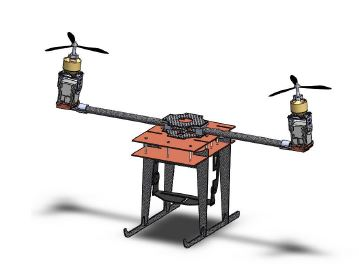
\includegraphics[height=3.5cm]{figuras/VANT1}
			\caption{Projeto mecânico VANT 1.0.}
			\label{vant1}
		\end{minipage}%
		\begin{minipage}{.5\textwidth}
			\centering
			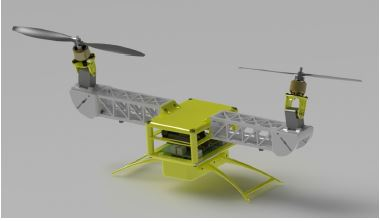
\includegraphics[height=3.5cm]{figuras/VANT2}
			\caption{Projeto mecânico VANT 2.0.}
			\label{vant2}
			\end{minipage}
	\end{figure}
					
	\begin{figure} [H]
		\centering
		\begin{minipage}{.5\textwidth}
			\centering
			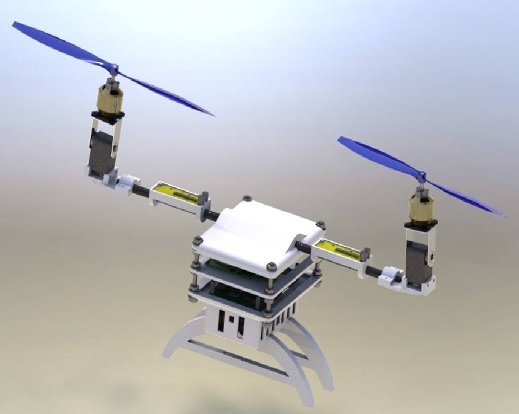
\includegraphics[height=3.5cm]{figuras/VANT21}
			\caption{Projeto mecânico VANT 2.1.}
			\label{vant21}
		\end{minipage}%
		\begin{minipage}{.5\textwidth}
			\centering
			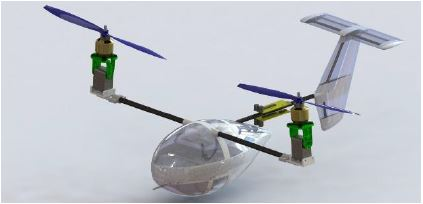
\includegraphics[height=3.5cm]{figuras/VANT3}
			\caption{Projeto mecânico VANT 3.0.}
			\label{vant3}
		\end{minipage}
	\end{figure}
								
	\begin{figure} [H]
		\centering
		\begin{minipage}{.5\textwidth}
			\centering
			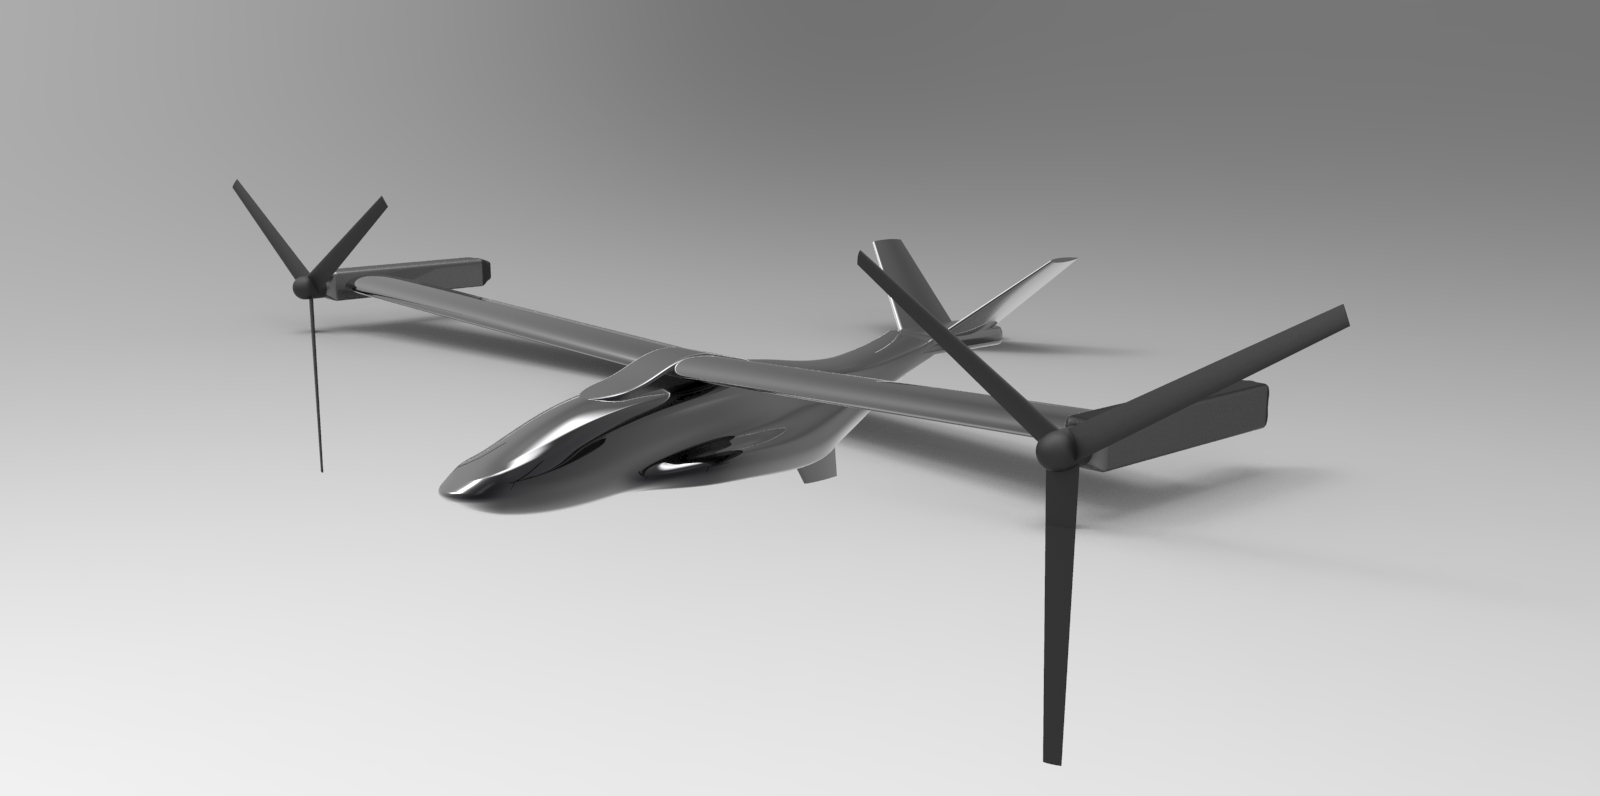
\includegraphics[height=3.5cm]{figuras/VANT4}
			\caption{Projeto mecânico VANT 4.0.}
			\label{vant4}
		\end{minipage}
	\end{figure}

O simulador ProVANT tem o objetivo de ser uma ferramenta confiável e de fácil utilização. O intuito é possibilitar a redução de custos e de tempo necessário para o projeto e validação de estratégias de controle.

\chapter{Instalação}

O simulador ProVANT é um ambiente de simulação desenvolvido com o objetivo de validar e avaliar o desempenho de estratégias de controle. A versão do simulador a qual esse manual se refere foi desenvolvida sobre as plataformas Gazebo 7 e o \textit{framework} de desenvolvimento de aplicações robóticas \textit{Robot Operating System} (ROS), na versão Kinect. Para utilizá-la é necessário um computador com \textbf{sistema operacional Ubuntu 16.04}

O ROS fornece uma interface de programação para aplicações em robótica e dispõe de repositórios com vários módulos de software. Já o Gazebo é um software de simulação 3D e de licença gratuita, atualmente sob a responsabilidade da Open Source Robotics Foundation (OSRF). Ele é capaz de simular o comportamento dinâmico de corpos rígidos articulados, e inclui funcionalidades como detecção de colisão e visualização gráfica.

Este capítulo apresenta os passos necessários para instalação do simulador ProVANT. Inicialmente, são detalhados os processos de instalação de plataformas utilizadas pelo simulador, como a biblioteca QT versão 5, os pacotes de software Git e ROS. Por fim, é apresentado o processo de instalação do ambiente de simulação ProVANT. 

\section{Procedimentos para instalação do simulador}

Os procedimentos especificados a seguir assumem como premissa que o computador, o qual será instalado o simulador, está rodando uma versão limpa/recém-instalada do Ubuntu versão 16.04. %Assegure-se que o computador esteja formatado antes de prosseguir nesta seção.

\subsection{Instalando Git}

O código fonte do simulador ProVANT está hospedado no Github. Para o acesso a esses arquivos é necessário primeiro que o usuário tenha instalado no computador o pacote Git. Caso não tenha, para instalá-lo, abra um novo terminal e execute os seguintes comandos:

%O código fonte do ambiente de simulação ProVANT está hospedado no Github. Os procedimentos para download do código fonte, conforme explicitado posteriormente nesta seção assume que o usuário tenha instalado no computador o pacote Git. 

\begin{bashcode}
$ sudo apt-get update
$ sudo apt-get install git
\end{bashcode}

\subsection{Instalando e configurando o ROS}

O ROS fornece uma interface de programação para aplicações de robótica e vários módulos de software, entre eles o simulador Gazebo na versão 7, utilizado pelo simulador ProVANT. Esta subseção detalha as instruções necessárias para a instalação da distribuição ROS Kinetic Kame.  A seguir estão detalhados os passos para a instalação do ROS\footnote{para mais detalhes sobre o processo de instalação, assim como problemas na instalação pode-se acessar a homepage do ROS, \url{wiki.ros.org}}.\\
\bigskip
\bigskip
\bigskip

\textbf{Configure os repositórios do Ubuntu} \\

Antes de iniciar a instalação é necessário configurar os repositórios do Ubuntu para níveis de permissão "restricted", "universe", e "multiverse.". Atenção: normalmente, após a instalação do Ubuntu 16.04, estas opções já se encontram configuradas. Caso não estejam, para obter instruções sobre como fazer isso siga o passo a passo apresentado em:
\begin{center}
\url{https://help.ubuntu.com/community/Repositories/Ubuntu}.
\end{center}

\textbf{Configure o sources.list} \\

Também é necessário configurar o computador para aceitar o software de packages.ros.org. Para isso, abra um novo terminal e digite o seguinte comando:

\begin{bashcode}
$ sudo sh -c 'echo "deb http://packages.ros.org/ros/ubuntu $(lsb_release -sc) main"
 >/etc/apt/sources.list.d/ros-latest.list'
\end{bashcode}

\textbf{Informe as chaves de criptografia para acesso aos repositórios do ROS} \\

Isso pode ser realizado executando o seguinte comando:

\begin{bashcode}
$ sudo apt-key adv --keyserver hkp://ha.pool.sks-keyservers.net:80 --recv-key 
421C365BD9FF1F717815A3895523BAEEB01FA116
\end{bashcode}

\textbf{Instalação} \\

Antes de iniciar o processo de instalação do ROS, é necessário atualizar o índice do pacote Debian, para isso execute:

\begin{bashcode}
$ sudo apt-get update
\end{bashcode}

Tendo atualizado os pacotes Debian, pode-se fazer download dos arquivos binários do ROS

\begin{bashcode}
$ sudo apt-get install ros-kinetic-desktop-full
\end{bashcode}

\textbf{Inicialize o Rosdep} \\

Antes de poder usar o ROS, é necessário inicializar o sistema Rosdep.  O sistema Rosdep permite instalar as dependências do sistema, para o código fonte que deseja-se compilar. Ele é necessário para executar alguns dos componentes principais no ROS.

\begin{bashcode}
$ sudo rosdep init
$ rosdep update
\end{bashcode}

\textbf{Configuração de variáveis de ambiente} \\

Para que as variáveis de ambiente do ROS sejam automaticamente adicionadas sempre que um novo terminal é iniciado, para isso execute os seguintes comandos:

\begin{bashcode}
$ echo "source /opt/ros/kinetic/setup.bash" >> $HOME/.bashrc
$ source $HOME/.bashrc
\end{bashcode}


\textbf{Crie um espaço de trabalho ROS}\\

Por fim, é necessário criar um espaço de trabalho ROS, para isso execute a seguinte sequência de comandos no terminal:

\begin{bashcode}
$ mkdir -p $HOME/catkin_ws/src
$ cd $HOME/catkin_ws/
$ catkin_make
$ source $HOME/catkin_ws/devel/setup.bash
$ echo "source $HOME/catkin_ws/devel/setup.bash" >> $HOME/.bashrc
\end{bashcode}

\subsection{Instalando a biblioteca QT}

%Para a instalação apropriada da interface gráfica de configuração do ambiente de simulação ProVANT é necessário a instalação da \textit{Integrated Development Environment} (IDE) Qt Creator 5. Para isso, acesse a url a seguir e faça download do pacote de instalação:
%\begin{center}
%\url{https://www.qt.io/download-open-source/?hsCtaTracking=f977210e-de67-475f-a32b-65cec207fd03%7Cd62710cd-e1db-46aa-8d4d-2f1c1ffdacea} 
%\end{center}

%Atenção: para realizar a instalação do pacote (com extensão ``.run''), é necessário fornecer permissão de execução ao arquivo de instalação. Assumindo que o arquivo se encontra na pasta ``\$HOME/Downloads'', com nome ``qt-unified-linux-x64-3.0.0-online.run'', este passo pode ser realizado a partir dos comandos: 

%\begin{bashcode}
%$ cd $HOME/Downloads
%$ sudo chmod +x qt-unified-linux-x64-3.0.0-online.run
%$ ./qt-unified-linux-x64-3.0.0-online.run
%\end{bashcode}

Para a instalação apropriada da interface gráfica de configuração do ambiente de simulação ProVANT, é necessária a instalação da \textit{Integrated Development Environment} (IDE) Qt Creator 5. Para isso, execute os seguintes comandos no terminal: 	

\small
\begin{bashcode}
$ cd $HOME/Downloads
$ wget http://download.qt.io/official_releases/online_installers/qt-unified-linux-x64-online.run
$ sudo chmod +x qt-unified-linux-x64-online.run
$ ./qt-unified-linux-x64-online.run
\end{bashcode}
\normalsize


\subsection{Download e instalação do ambiente de simulação}

O código fonte do ambiente de simulação ProVANT, está localizado no repositório: 

\begin{center}
\url{https://github.com/Guiraffo/ProVANT-Simulator}
\end{center}

\noindent Este repositório possui acesso particular, então, antes de prosseguir como processo de instalação, solicite acesso ao Prof. Guilherme Vianna Raffo\footnote{E-mail para contato: raffo@ufmg.br}.

Com o acesso liberado, para fazer o download da versão atual do ambiente de simulação ProVANT, basta digitar no terminal os seguintes comandos:

\begin{bashcode}
$ cd $HOME/catkin_ws/src
$ git clone https://github.com/Guiraffo/ProVANT-Simulator.git
\end{bashcode}

Tendo realizado o download pode-se realizar a instalação e configuração do ambiente de simulação através da execução dos seguintes comandos:

\begin{bashcode}
$ cd $HOME/catkin_ws/src/ProVANT-Simulator
$ sudo chmod +x install.sh
$ ./install.sh
\end{bashcode}


Caso todos os procedimentos descritos anteriormente tenham sido realizados com sucesso, o usuário estará pronto para prosseguir para o próximo capítulo, referente ao fluxo de utilização do ambiente de simulação ProVANT.

\chapter{Fluxo de utilização}

Este capítulo apresenta as funcionalidades disponíveis para a operação do simulador através da interface gráfica, tais quais:

\begin{itemize}
\setlength{\itemsep}{1pt}
\setlength{\parskip}{0pt}
\setlength{\parsep}{0pt}
\item Seleção de cenário
\item Seleção de modelo de VANT
\item Configuração de cenário
\item Edição de configurações do VANT
\item Inicialização de simulação.
\item Exemplos
\end{itemize}
 
\section{Como inicializar o ambiente de simulação}

Tendo realizado o processo de instalação do simulador com exito, como descrito no capítulo anterior, pode-se iniciar o processo de desenvolvimento de controladores no ambiente de simulação ProVANT. Para iniciar a interface gráfica do usuário abra um novo terminal e digite o seguinte comando:

\begin{bashcode}
$ provant_gui
\end{bashcode}

A interface gráfica de acesso ao simulador será então incializada e aparecerá a janela principal, como ilustrado na Figura \ref{1}.

\begin{figure*}[!ht]
	\centering
	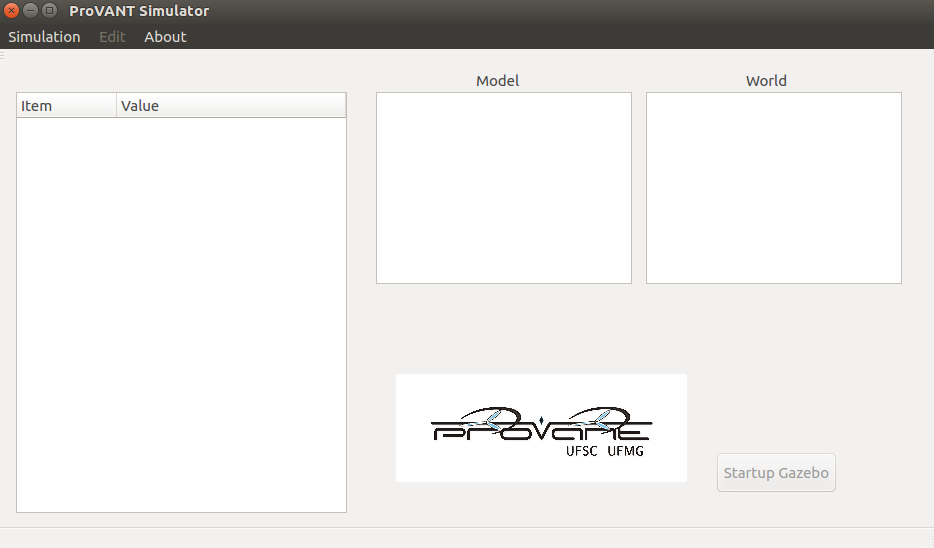
\includegraphics[width=0.8\columnwidth]{figuras/1.png}
	\caption{Janela inicial.}
	\label{1}
\end{figure*}

\section{Seleção de cenário}

Tendo inicializado a interface gráfica do ambiente de simulação, é necessário que o usuário selecione um cenário de simulação. Isso pode ser realizado de duas maneiras diferentes, ambas através da utilização da opção "Simulation", presente no menu superior da interface gráfica, ilustrado na figura \ref{2}: 

\begin{figure*}[!ht]
	\centering
	
\includegraphics[width=100pt]{figuras/2.png}
	\caption{Menu superior.}
	\label{2}
\end{figure*}

\begin{itemize}
	\item[(i)] Ao clicar em "New", é possível abrir um cenário template com extensão ".tpl".
	
	Um cenário template é um uma configuração de cenário que serve de molde para a criação de outros cenários. Ele não pode ser editado, necessita da adição de um modelo de um VANT e deve ser salvo antes da simulação com o formato ".world"
	 
	\item[(ii)] Ao clicar em "Open", é possível abrir um cenário já existente (arquivo com extensão ".world").  
	
	\item[(iii)] Ao clicar em "About", é possível conferir informações gerais do simulador ProVANT .  
\end{itemize}
  
Ainda no menu "Simulation", é possível salvar um cenário com outro nome no formato ".world", clicando em ("Save"), e também finalizar o ambiente de simulação, clicando em ("Exit").

\section{Seleção do VANT}

Através da opção "Edit", no menu superior, é possível selecionar modelo de VANT a ser utilizado na simulação. Atenção: nessa versão do ambiente de simulação, é possível apenas a adição de de um único VANT na mesma instância de simulação.

\section{Janela de configuração da simulação}

Tendo escolhido o VANT e o cenário de simulação, suas imagens a imagem ilustrativa do cenário aparecerá na interface e portanto é possível verificar se foram selecionados corretamente, como mostra a Figura \ref{tela_inicial.jpg}, através dos itens (2) e (3), respectivamente. 
% É possível também visualizar parâmetros e configurações de itens relacionados aos mesmos, como gravidade, posição e orientação iniciais, etc. 

\begin{figure*}[!ht]
	\centering
	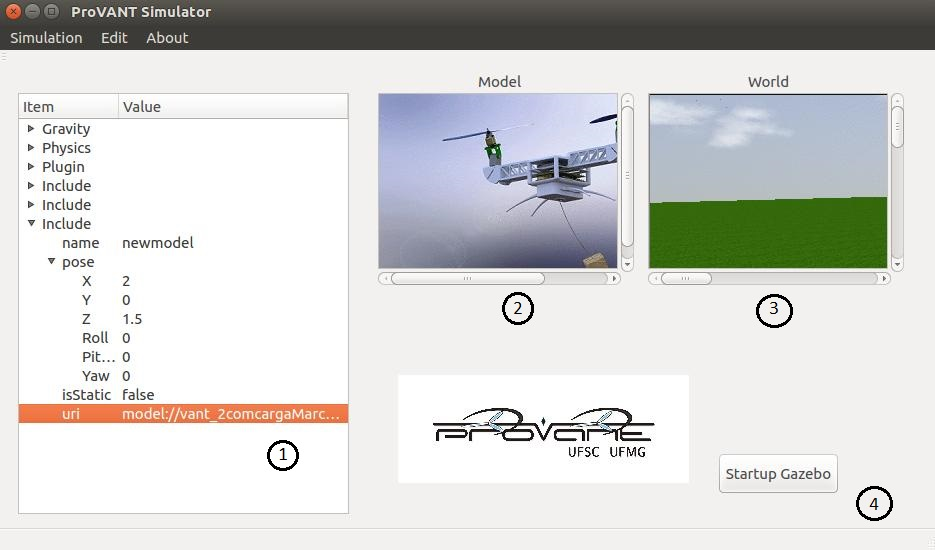
\includegraphics[width=500pt]{figuras/tela_inicial.jpg}
	\caption{Janela de configuração da simulação.}
	\label{tela_inicial.jpg}
\end{figure*}

Ainda com relação à Figura \ref{tela_inicial.jpg}, o item (1) corresponde à uma árvore de informações e configurações do VANT e do cenário de simulação. Através de duplo clique em cima do campo desejado é possível realizar configurações. Os campos dessa arvore são:

\begin{itemize}
	\item Gravity: vetor de aceleração da gravidade com relação ao referencial do mundo em $m/s^2$; 
	\item Physics: motor físico física utilizada para realizar simulação. As opções possíveis são:
	\begin{itemize}
		\setlength{\itemsep}{1pt}
		\setlength{\parskip}{0pt}
		\setlength{\parsep}{0pt}
		\item ode (propositório de criação: dinâmica simplificada para robôs)
		\item bullet (propositório de criação: jogos)
		\item dart: (propositório de criação: computação gráfica e controle de robôs)
		\item simbody (propositório de criação: plicações biomecânicas)
	\end{itemize}
	\item name: Nome do modelo do VANT no simulador Gazebo.;
	\item pose: Posição (x,y,z) e orientação (roll,pitch,yaw) iniciais do VANT, em $m$ e $rad$, respectivamente.   
\end{itemize}

\noindent Através do duplo clique no campo uri, uma nova janela se abrirá, na qual é possível visualizar e realizar configurações no modelo, controlador, atuadores e sensores. Mais detalhes sobre está janela são apresentados na próxima seção. O item (4) permite a inicialização da simulação com as configurações, modelo e cenário selecionados pelo usuário na interface gráfica.

%Os itens número 2 e 3 correspondem, respectivamente, as imagens que ilustram o VANT e o cenário selecionados para simulação.

\section{Janela de visualização e configuração dos parâmetros do modelo, estratégia de controle e instrumentação}
\label{SecEstCtrl}

Como mencionado, através de duplo clique no campo uri uma nova janela de configurações será aberta, como mostra a Figura \ref{4}. Através das quatro abas disponíveis: Parameters, Controller, Sensors e Actuators; é possível gerenciar as configurações do modelo, estratégia de controle e instrumentação utilizados para simulação. A janela é inicializada com a aba Parameters selecionada. Esta aba permite a visualização dos parâmetros do modelo do VANT utilizado na simulação.

\begin{figure*}[!ht]
	\centering
	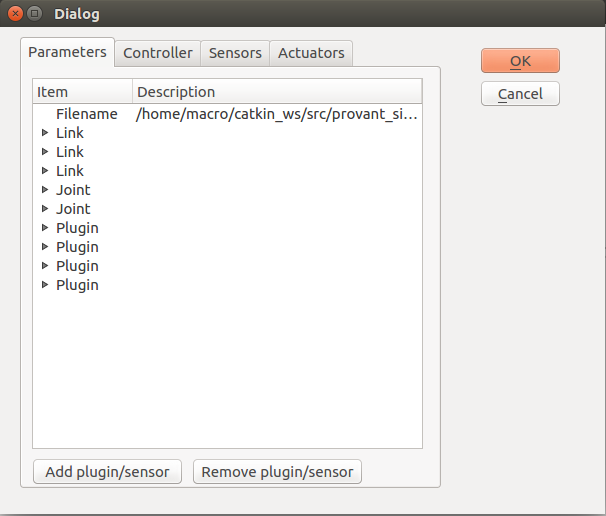
\includegraphics[width=250pt]{figuras/4.png}
	\caption{Aba para visualização dos parâmetros do modelo do VANT.}
	\label{4}
\end{figure*}

A Figura \ref{5} mostra a aba "Controller". Nela é possível criar uma nova estratégia de controle, utilizando o item (2), selecionar uma existente, através do item (3) ou compilá-las, item (4). A estratégia de controle selecionada para ser utilizada na simulação é mostrada no item (1). Mais detalhes sobre esses itens são descritos a seguir.

\begin{figure*}[!ht]
	\centering
	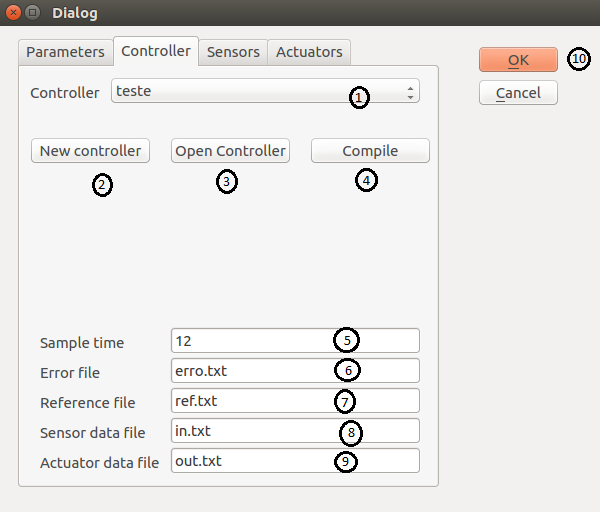
\includegraphics[width=250pt]{figuras/5_2.png}
	\caption{Aba para seleção e configuração da estratégia de controle.}
	\label{5}
\end{figure*}

\subsubsection{Criando uma nova estratégia de controle}

Para criar uma nova estratégia de controle, deve-se clicar no botão "New controller" $~$ item (2), e uma nova janela será mostrada (Figura \ref{9}). Nesta janela, o usuário deve inserir o nome da nova estratégia de controle (mais detalhes sobre a criação de uma nova estratégia de controle são apresentados no Capítulo \ref{controle}).

\begin{figure*}[!ht]
	\centering
	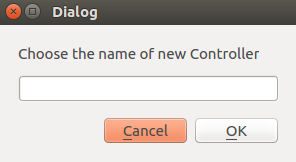
\includegraphics[width=100pt]{figuras/9.png}
	\caption{Criando uma nova estratégia de controle.}
	\label{9}
\end{figure*}

\subsubsection{Modificando uma estratégia de controle já existente}

Para modificar uma estratégia de controle já existente, o usuário deve selecionar o nome da estrategia de controle entre várias listadas na caixa de listagem item (1) e clicar na botão "Open controller" item (3). Após escolher a estratégia, o gerenciador de arquivos Nautilus será aberto no diretório com todos os arquivos e diretórios associados ao controlador, conforme mostra a Figura \ref{10}.

% (colocar uma figura com essa janela e citar ela).%

\begin{figure*}[!ht]
	\centering
	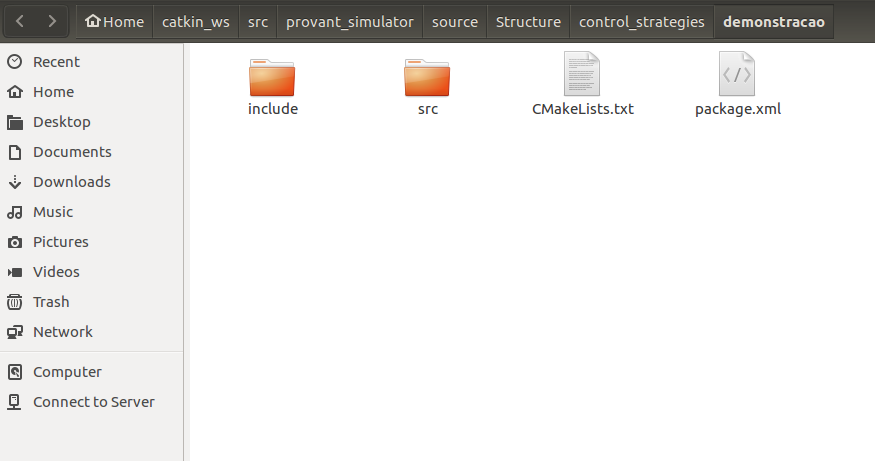
\includegraphics[width=300pt]{figuras/10.png}
	\caption{Diretório contendo arquivos e pastas associados à estratégia de controle a ser modificada.}
	\label{10}
\end{figure*}

\subsubsection{Compilando o controlador}

Para compilar o código associado à estratégia de controle selecionada, o usuário deve clicar no botão "Compile" $~$ item (4). \textbf{Esta etapa deve ser realizada sempre que haja modificações na estratégia de controle}. Caso ocorram erros durante a compilação, o relatório de saída do compilador será mostrado em um arquivo de texto por meio do aplicativo gedit.

\subsubsection{Alterando configurações adicionais }

A aba ''Controller'' também permite a configuração de outros parâmetros associados à simulação. O campo ''Sample time'', item (5), permite a configuração do perído de amostragem em milissegundos. Já os demais campos, ''Error file'', item (6), ''Reference data file'', item (7), ''Sensor file'', item (8) e ''Actuator data file'', item (9) determinam o nome dos arquivos de texto onde serão registrados os valores do erro dos estados, trajetória desejada, dados dos sensores e sinais de controle, respectivamente. Estes arquivos podem ser carregados diretamente no MATLAB. Tais arquivos estarão disponíveis no diretório: 

\begin{bashcode}
$HOME/catkin_ws/srcProVANT-Simulator/source/Structure/Matlab
\end{bashcode}

\subsection{Selecionando a instrumentação disponível}
\label{sensoresatuadores}

As abas Sensors e Actuators, ilustradas na Figura \ref{6}, listam, respectivamente, os nomes dos tópicos dos sensores e atuadores que o controlador terá acesso durante a simulação \textbf{de acordo a ordem apresentada}. Tais tópicos são configurados durante a configuração dos plugins, sendo melhor detalhados na seção \ref{plugins}. 

Conforme necessário, o usuário deve adicionar, remover e editar os intrumentos (atuadores/sensores) disponíveis na lista. Para adicionar novos instrumentos basta selecionar o botão ''Add'' e clicar duas vezes no nome do instrumento desejado. Para removê-los, basta selecionar o instrumento e pressionar o botão ''Remove''. 

\begin{figure}
	\hfill
	\subfloat{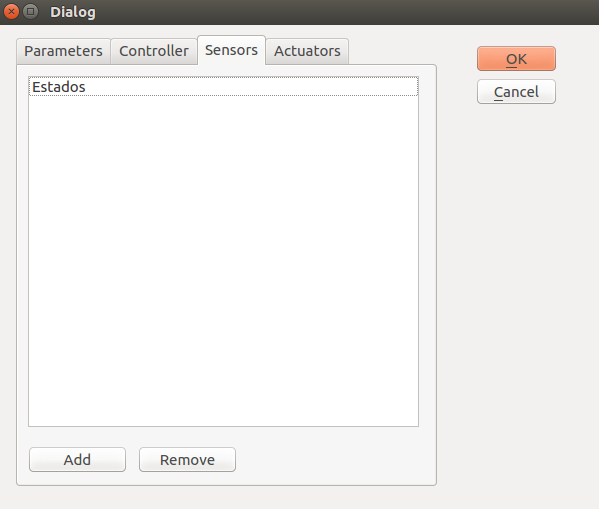
\includegraphics[width=230pt]{figuras/6.png}}
	\hfill
	\subfloat{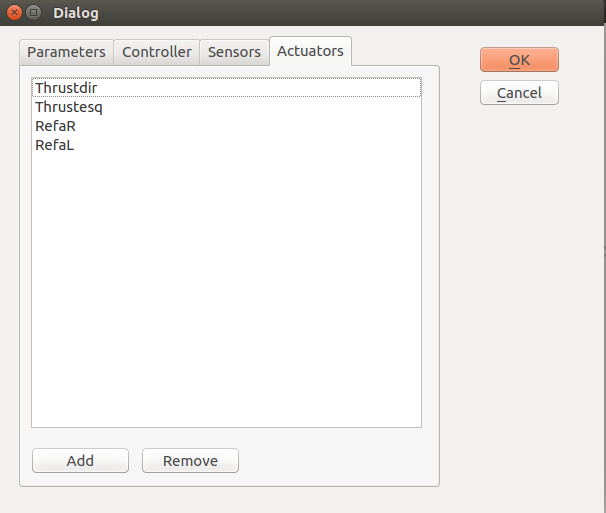
\includegraphics[width=230pt]{figuras/7.png}}
	\hfill
	\caption{Abas para seleção da instrumentação disponível durante a simulação.}
	\label{6}
\end{figure}


\subsection{Inicializando a simulação}

Após realizar todas as configurações, o usuário deve pressionar o botão "OK" $~$ item (10). A janela de configuração da simulação (Figura \ref{tela_inicial.jpg}) será mostrada novamente. A simulação pode ser então inicializada com o modelo de VANT, cenário, estratégia de controle e instrumentação selecionados, através do botão "Startup Gazebo" $~$, item (4) da Figura \ref{tela_inicial.jpg}. O simulador Gazebo será inicializado, conforme mostrado na Figura \ref{12}. 



\begin{figure*}[!ht]
	\centering
	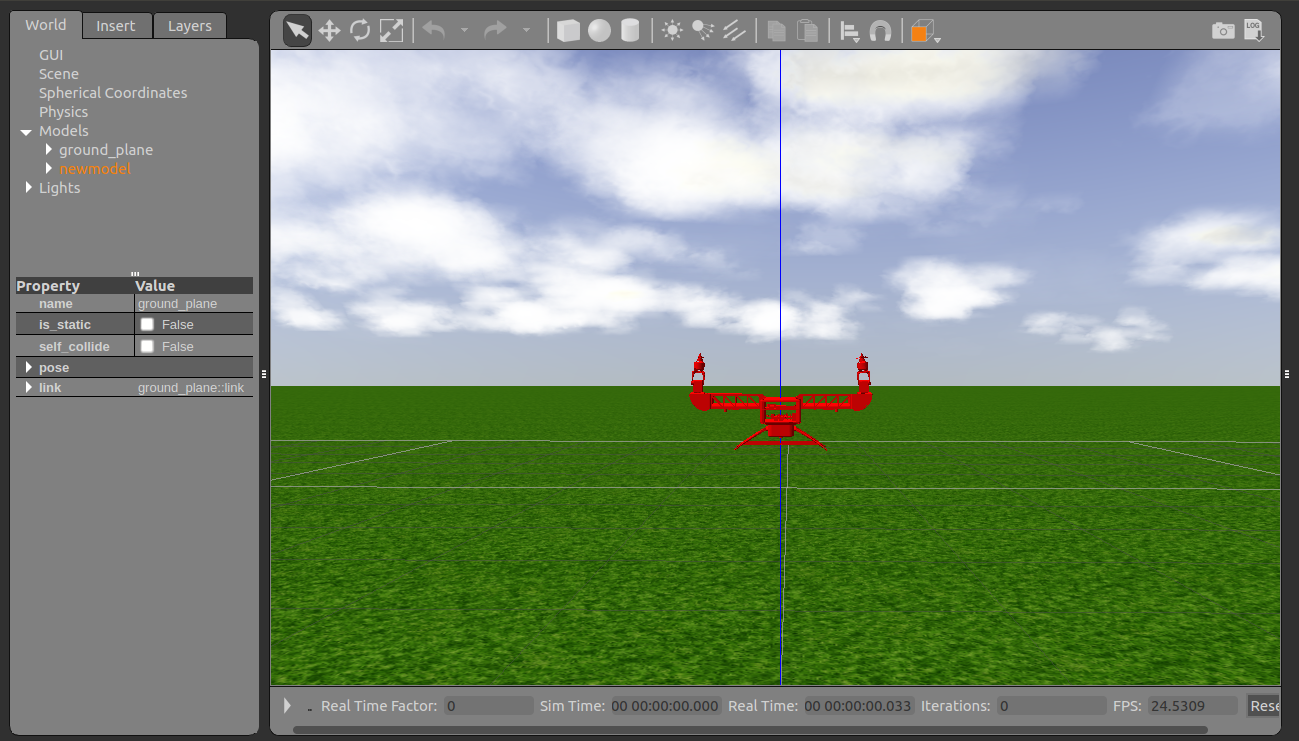
\includegraphics[width=400pt]{figuras/12.png}
	\caption{Janela inicial do simulador Gazebo.}
	\label{12}
\end{figure*}

Para dar início à simulação, o usuário deve pressionar o botão STEP. \textbf{O botão PLAY não deve ser utilizado}.


\section{Exemplos}


		\subsection{VANT 4.0}

Para executar a simulação do vant 4.0 o usuário deve primeiro selecionar no menu superior da interface gráfica a opção "Open" e abrir o cenário existente "vant4.world". Em seguida, no menu superior da interface gráfica, através da opção "Edit", o usuário deve selecionar o modelo do VANT 4.0. A pose do VANT deverá aparecer na janela de configuração da simulação de acordo com o que foi definido no arquivo "vant4.world", no caso do VANT 4.0 essa pose é 
Posição($0,4,0$) e Orientação($0,0,0$).

\begin{figure*}[!ht]
	\centering
	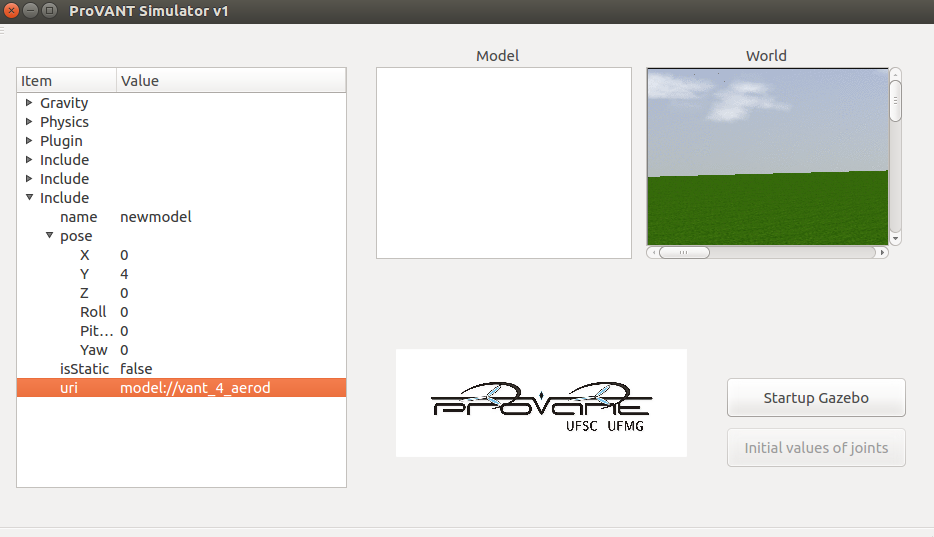
\includegraphics[width=250pt]{figuras/v4gui.png}
	\caption{Tela Inicial da Interface Gráfica para VANT 4.0.}
	\label{13}
\end{figure*}

Por fim, através do duplo clique no campo uri, uma janela para configurar modelo, controlador, atuadores e sensores se abrirá. Na aba "Controller" deve-se selecionar o controlador "vant4Winf" e selecionar o botão "Compile". 


\begin{figure*}[!ht]
	\centering
	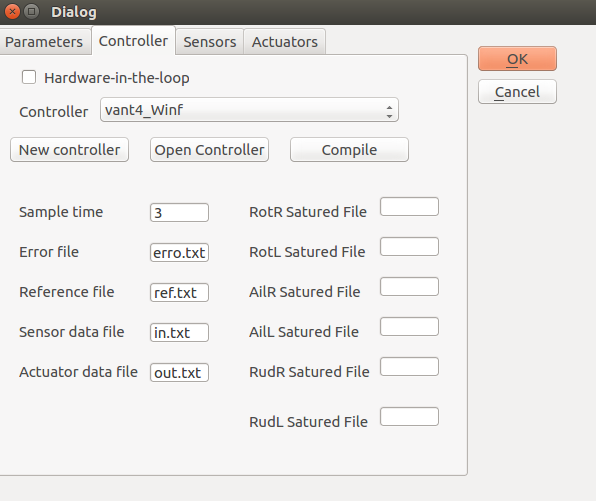
\includegraphics[width=150pt]{figuras/v4controllersetup.png}
	\caption{Tela para Configurar Estrategia de Controle para o VANT 4.0.}
	\label{14}
\end{figure*}


Agora a simulação esta configurada e o usuário deve selecionar a opção "Startup Gazebo" na tela inicial da interface gráfica o que levará a inicializar o Gazebo, onde o usuário deverá apertar a opção "step" para iniciar a simulação.


\begin{figure*}[!ht]
	\centering
	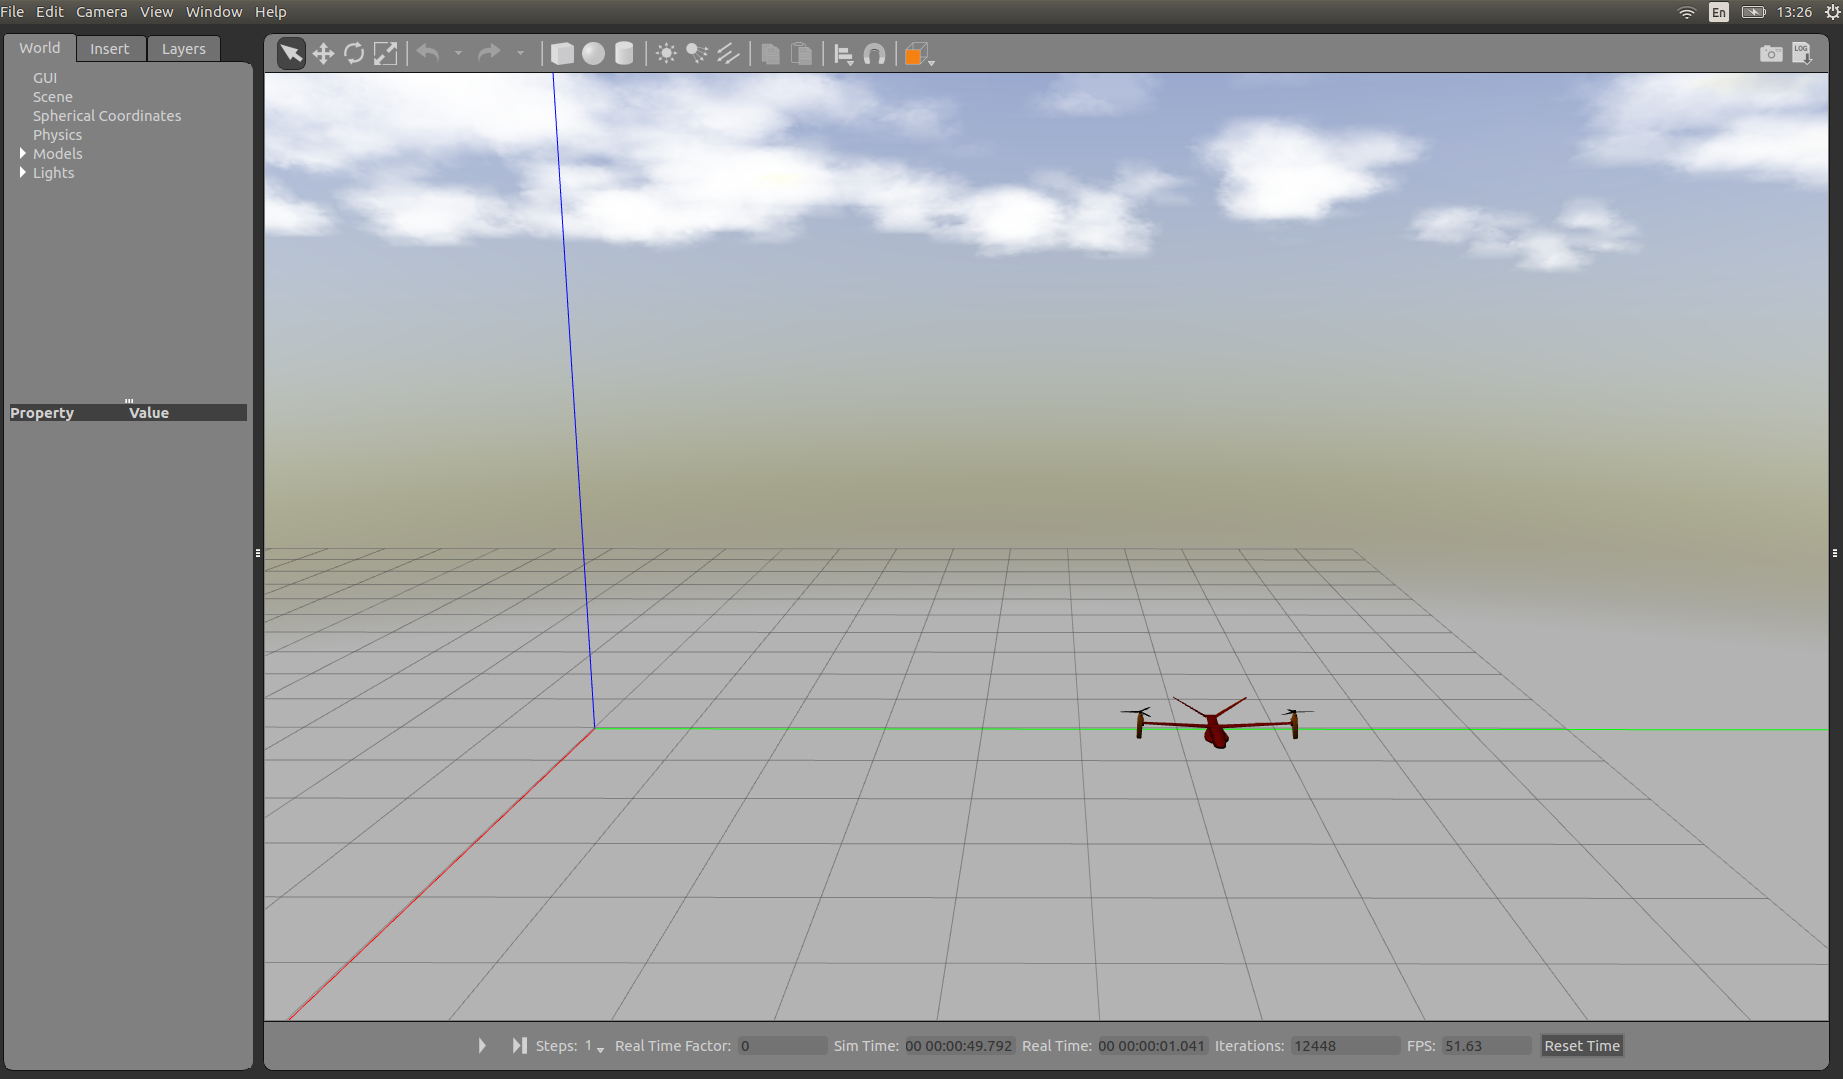
\includegraphics[width=350pt]{figuras/v4sim.png}
	\caption{Simulação do VANT 4.0.}
	\label{15}
\end{figure*}


Com o plugin "DataSaveTiltRotor", explicado na seção \textbf{B}, é possivel salvar os valores das forças aplicadas durante a simulação assim como os valores da inclinação dos rotores, deflexão dos \textit{ailerons} e deflexão dos \textit{rudders} são salvos em arquivos ".txt" no diretório:
\begin{bashcode}
	$HOME/catkin_ws/srcProVANT-Simulator/source/Structure/Matlab
\end{bashcode}

Além disso no mesmo diretório os valores do erro dos estados, trajetória desejada, dados dos sensores e sinais de controle podem ser encontrados em arquivos ".txt". 

	\subsection{VANT 4.0 com Cenário}

Para utilizar o VANT 4.0 com seu cenário disponibilizado pra simulação primeiro deve-se selecionar no menu superior da interface gráfica a opção "Open" e abrir o cenário existente "hill.world"


\begin{figure*}[!ht]
	\centering
	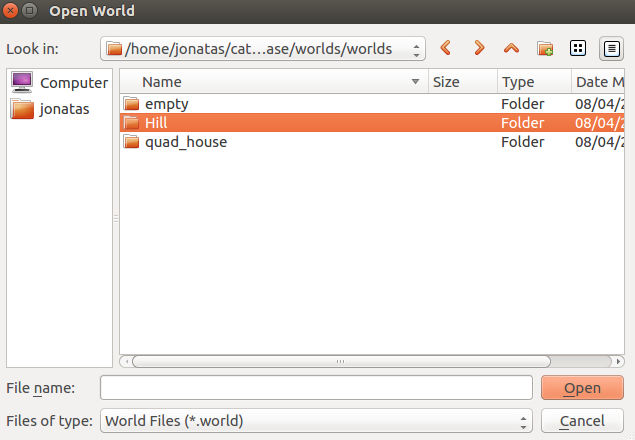
\includegraphics[width=250pt]{figuras/cenarioworld.png}
	\caption{Simulação do VANT 4.0.}
	\label{16}
\end{figure*}


Não é necessário adicionar o VANT 4.0 através do menu superior "Edit" como feito no exemplo anterior. O próximo passo é na tela inicial da interface gráfica clicar duas vezes no campo uri e, da mesma forma que no exemplo VANT 4.0, na aba "Controller" deve-se selecionar o controlador "vant4Winf" e selecionar o botão "Compile". 


A tela inicial da interface gráfica deve estar com Posição($0,0,0$) e Orientação($0,0,0$) como mostra a figura:

\begin{figure*}[!ht]
	\centering
	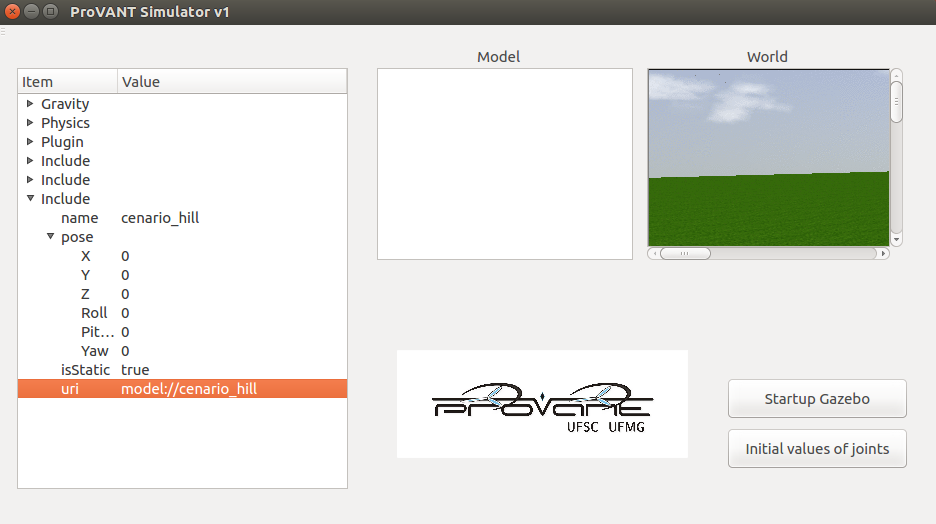
\includegraphics[width=250pt]{figuras/cenariogui.png}
	\caption{Tela Inicial da Interface Gráfica para VANT 4.0 com Cenário.}
	\label{17}
\end{figure*}

Agora a simulação esta configurada e o usuário deve selecionar a opção "Startup Gazebo" na tela inicial da interface gráfica o que levará a inicializar o Gazebo, onde o usuário deverá apertar a opção "step" para iniciar a simulação do VANT 4.0 no cenário disponibilizado.

\begin{figure*}[!ht]
	\centering
	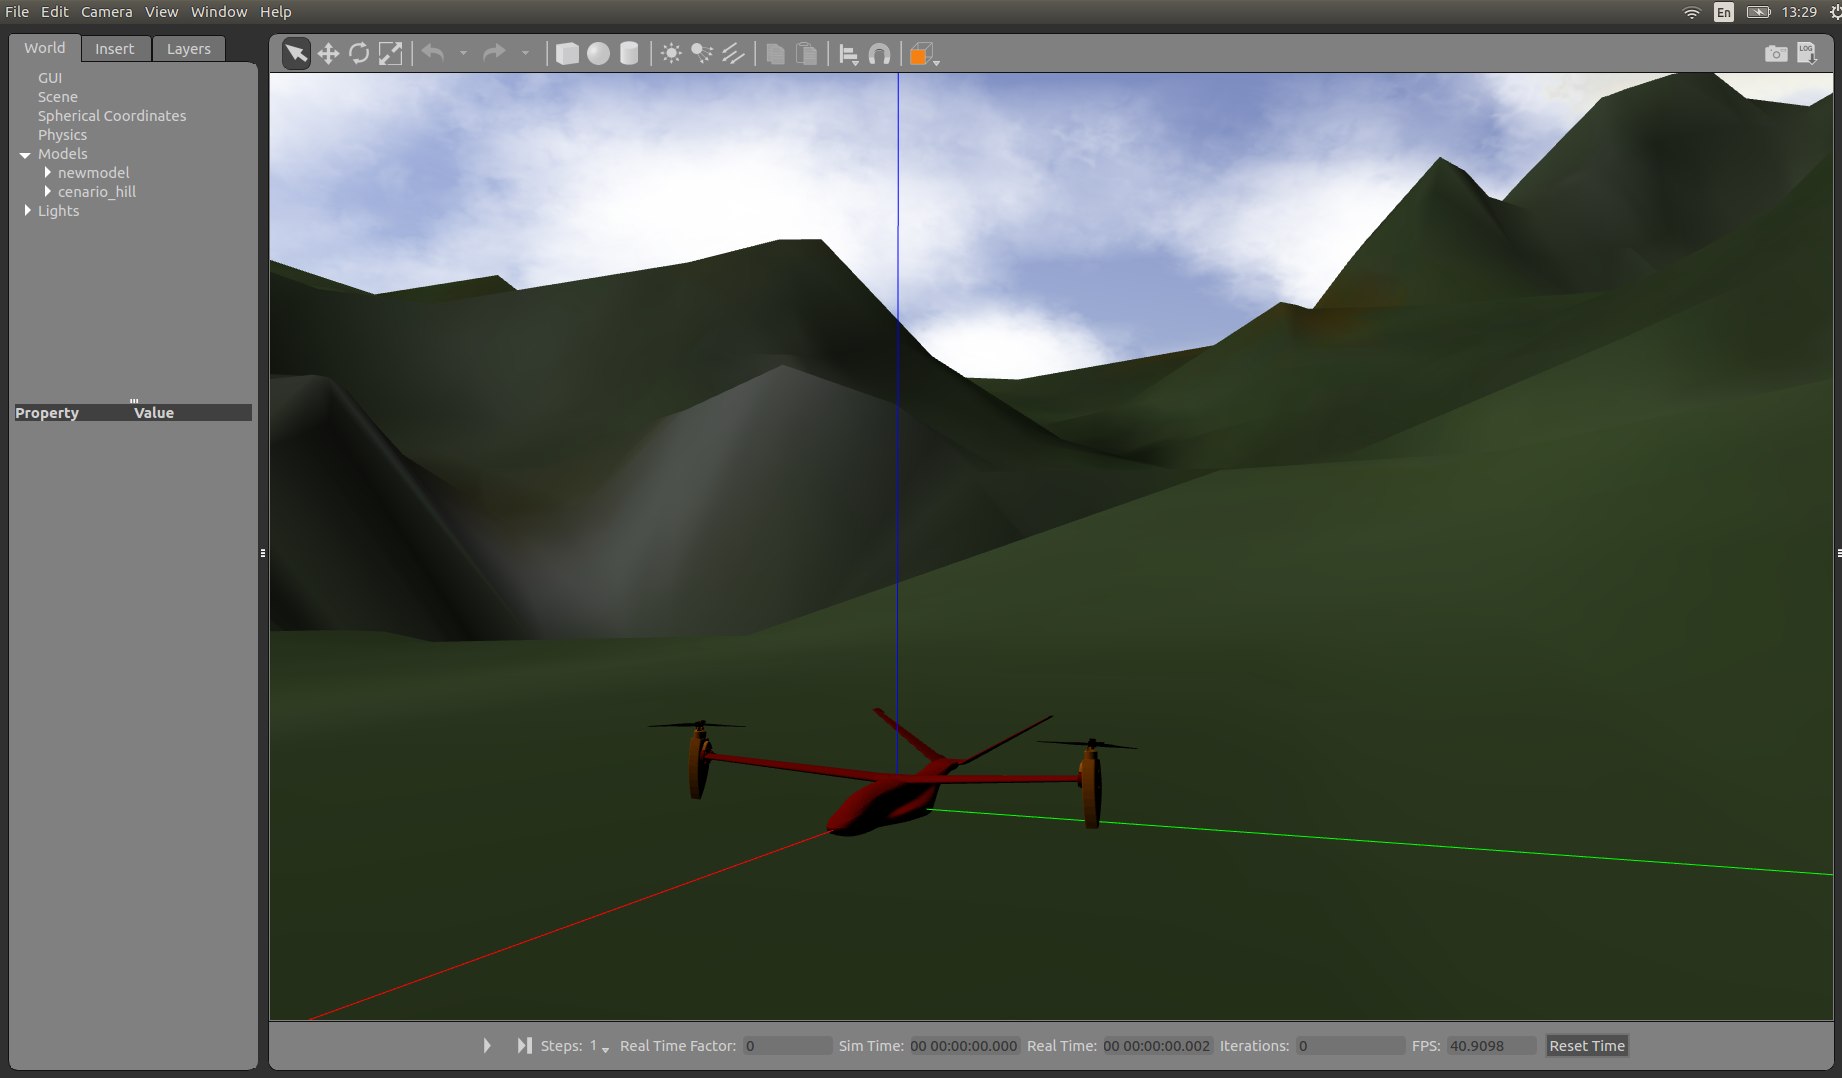
\includegraphics[width=250pt]{figuras/cenariosim.png}
	\caption{Simulação do VANT 4.0 com Cenário.}
	\label{18}
\end{figure*}

		\subsection{Visualizar Trajetória do VANT 4.0 no Rviz}

Para visualizar a trajetória do VANT no Rviz o usuário deve primeiro seguir os passos mostrados nos exemplos \textbf{VANT 4.0} ou \textbf{VANT 4.0 com Cenário}. Depois, em um terminal, o usuário deve inicializar o rviz para configura-lo.

\begin{bashcode}
	$ rosrun rviz rviz
	\end{bashcode}

A seguinte tela deverá ser visualizada no rviz:


\begin{figure*}[!ht]
	\centering
	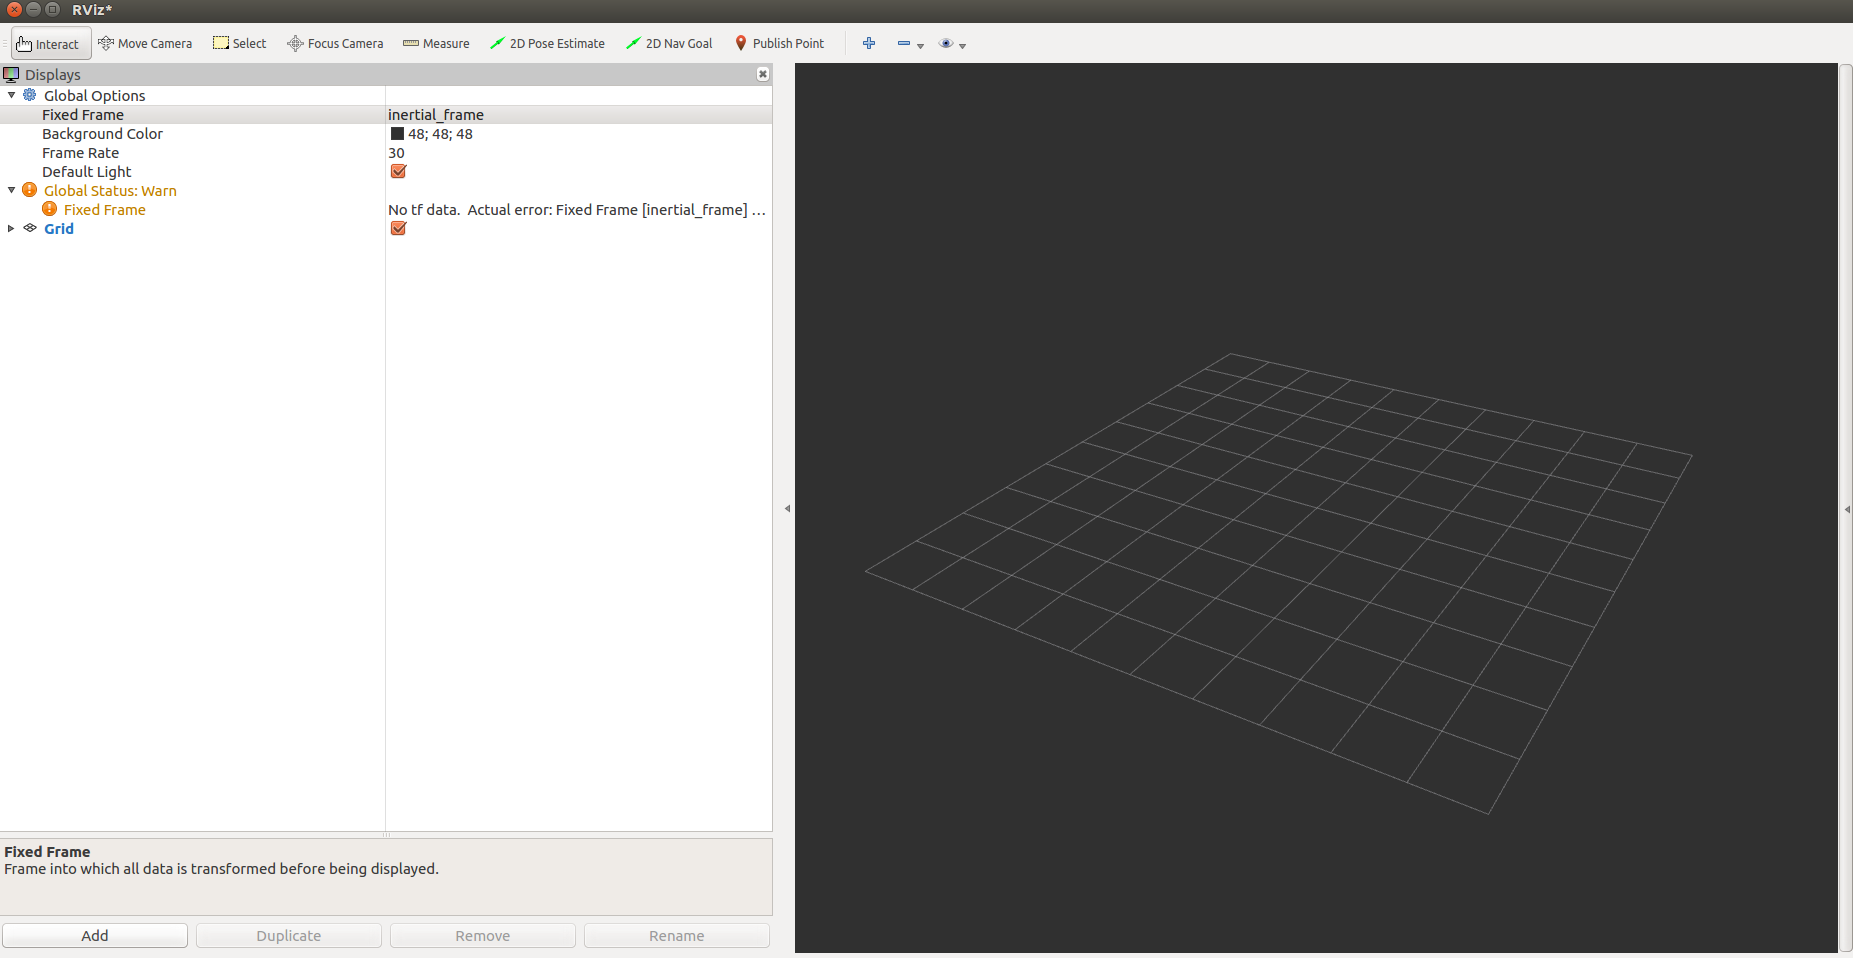
\includegraphics[width=450pt]{figuras/rvizconfig1.png}
	\caption{Tela Inicial do Rviz.}
	\label{19}
\end{figure*}

A opção "\textit{fixed frame}" deverá ser escolhida como "\textit{inertial frame}". Em seguida deve-se selecionar o botão "Add" na parte esquerda inferior da janela de configurações do Rviz e escolher a opção "Path".


\begin{figure*}[!ht]
	\centering
	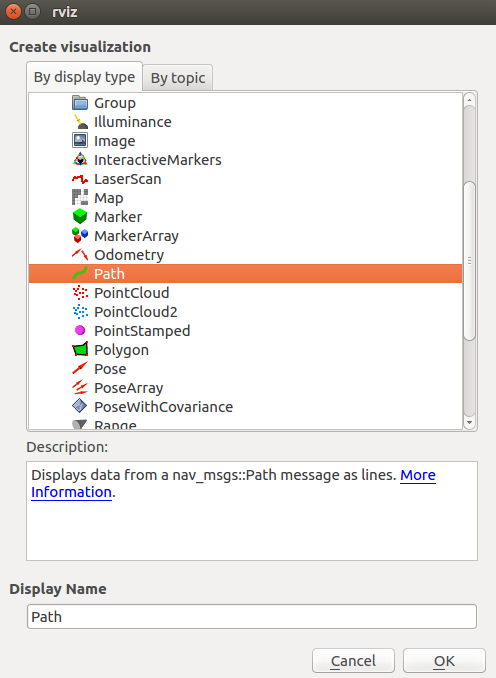
\includegraphics[width=150pt]{figuras/rvizconfig.png}
	\caption{Displays.}
	\label{20}
\end{figure*}

Para configurar o display "Path" é fácil e intuitivo basta configurar três parâmetros: "topic", "Buffer Length" e "Pose Style". Em "Topic" deve-se selecionar o tópico responsável por mostrar a \textit{trajetória real} que o VANT faz, o tópico \textit{/Path}. Altos valores de "Buffer Length" permitem que a trajetória fique visível por mais tempo, um valor de $12000$ é o suficiente.Para valores menores a trajetória se parecerá mais como um rastro perseguindo o VANT. O ultimo parâmetro é "Pose Style" que deve ser selecionado como \textit{Arrow}. Modificando os subparâmetros desse parâmetro é possível configurar a forma da trajetória que melhor satisfaça o usuário.


\begin{figure*}[!ht]
	\centering
	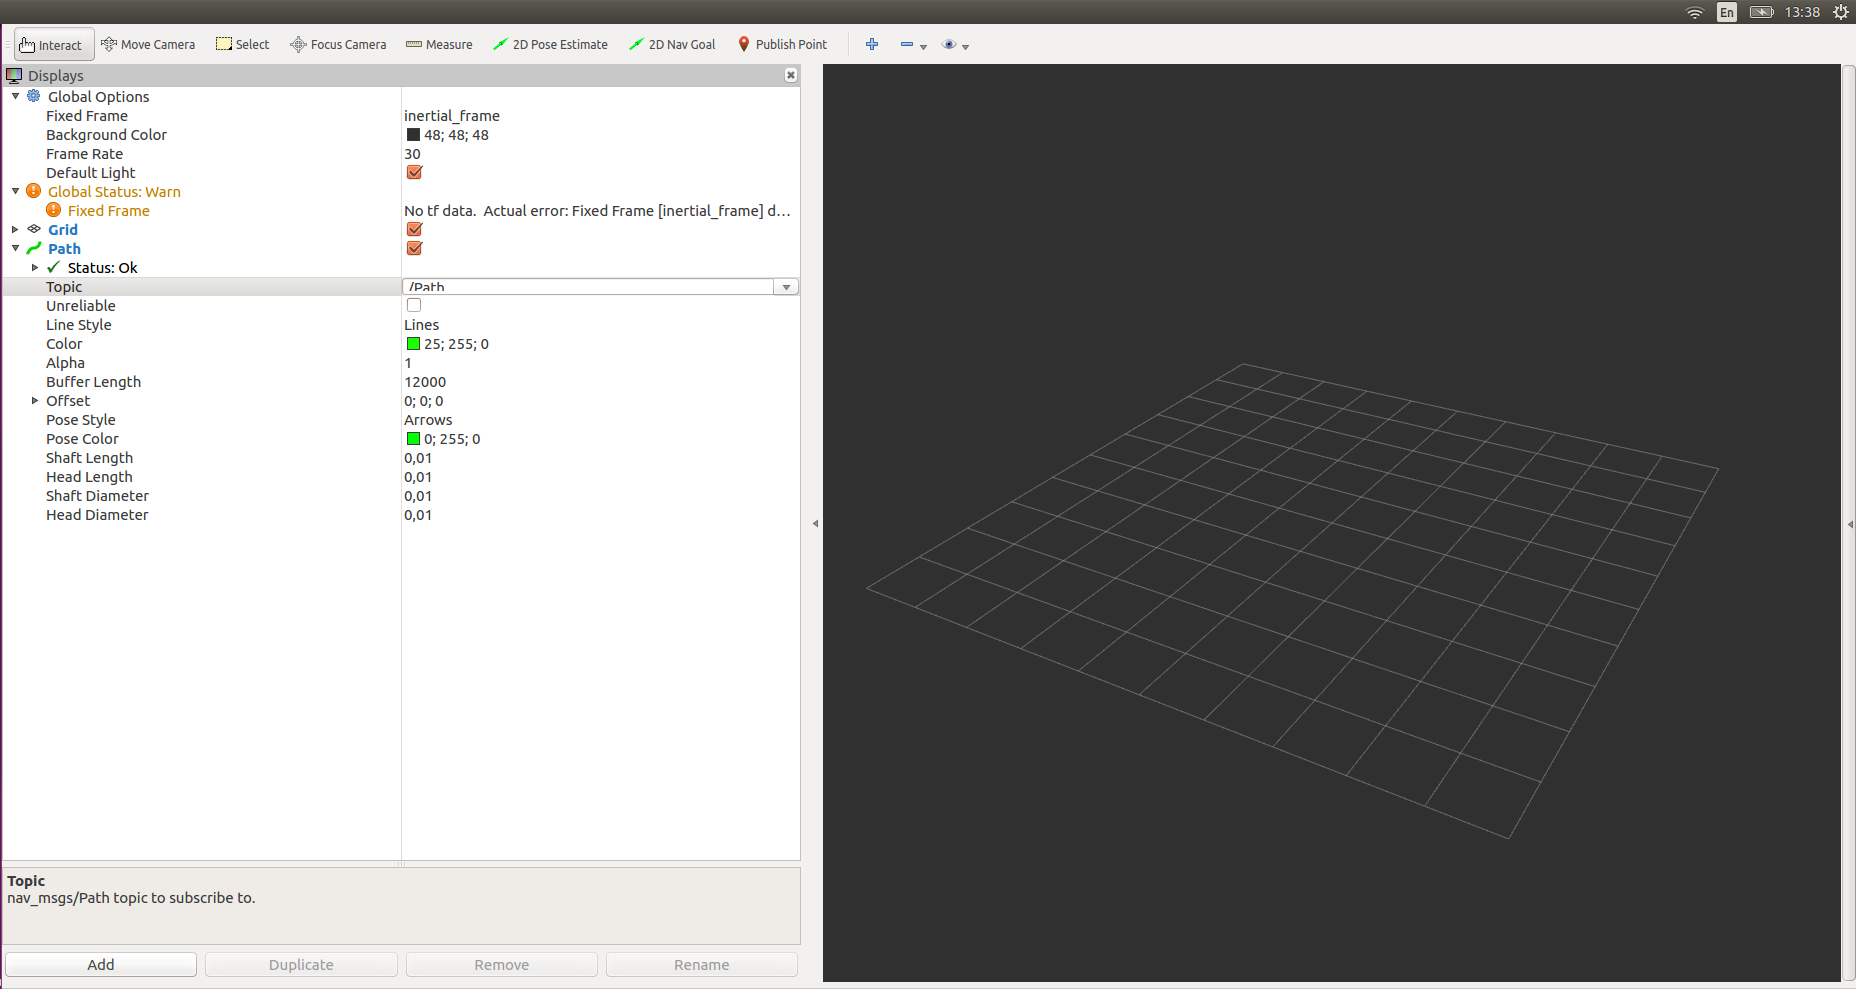
\includegraphics[width=450pt]{figuras/rvizconfig2.png}
	\caption{Configuração do Display \textit{/Path}.}
	\label{21}
\end{figure*}

Dentre as configurações pode-se também alterar a cor da trajetória. Uma vez configurado o display Path que mostra a trajetoria real, deve-se selecionar o botão "Add" no menu inferior esquerdo da janela de configurações do Rviz e adicionar outro Display Path. Dessa vez o display Path deve ser configurado para mostrar a \textit{trajetória de referência} o que é feito da mesma forma que para a \textit{trajetória real} mudando apenas o parametro "Topic" para \textit{/Path ref}.

Por fim, o usuário novamente deve selecionar a opção "Add" no menu inferior esquerdo da janela de configurações do Rviz e selecionar o Display "Marker". O único parâmetro a ser configurado é o "Topic", que deve ser selecionado como \textit{/marker}. A figura 3.19 mostra esse processo.
\begin{figure*}[!ht]
	\centering
	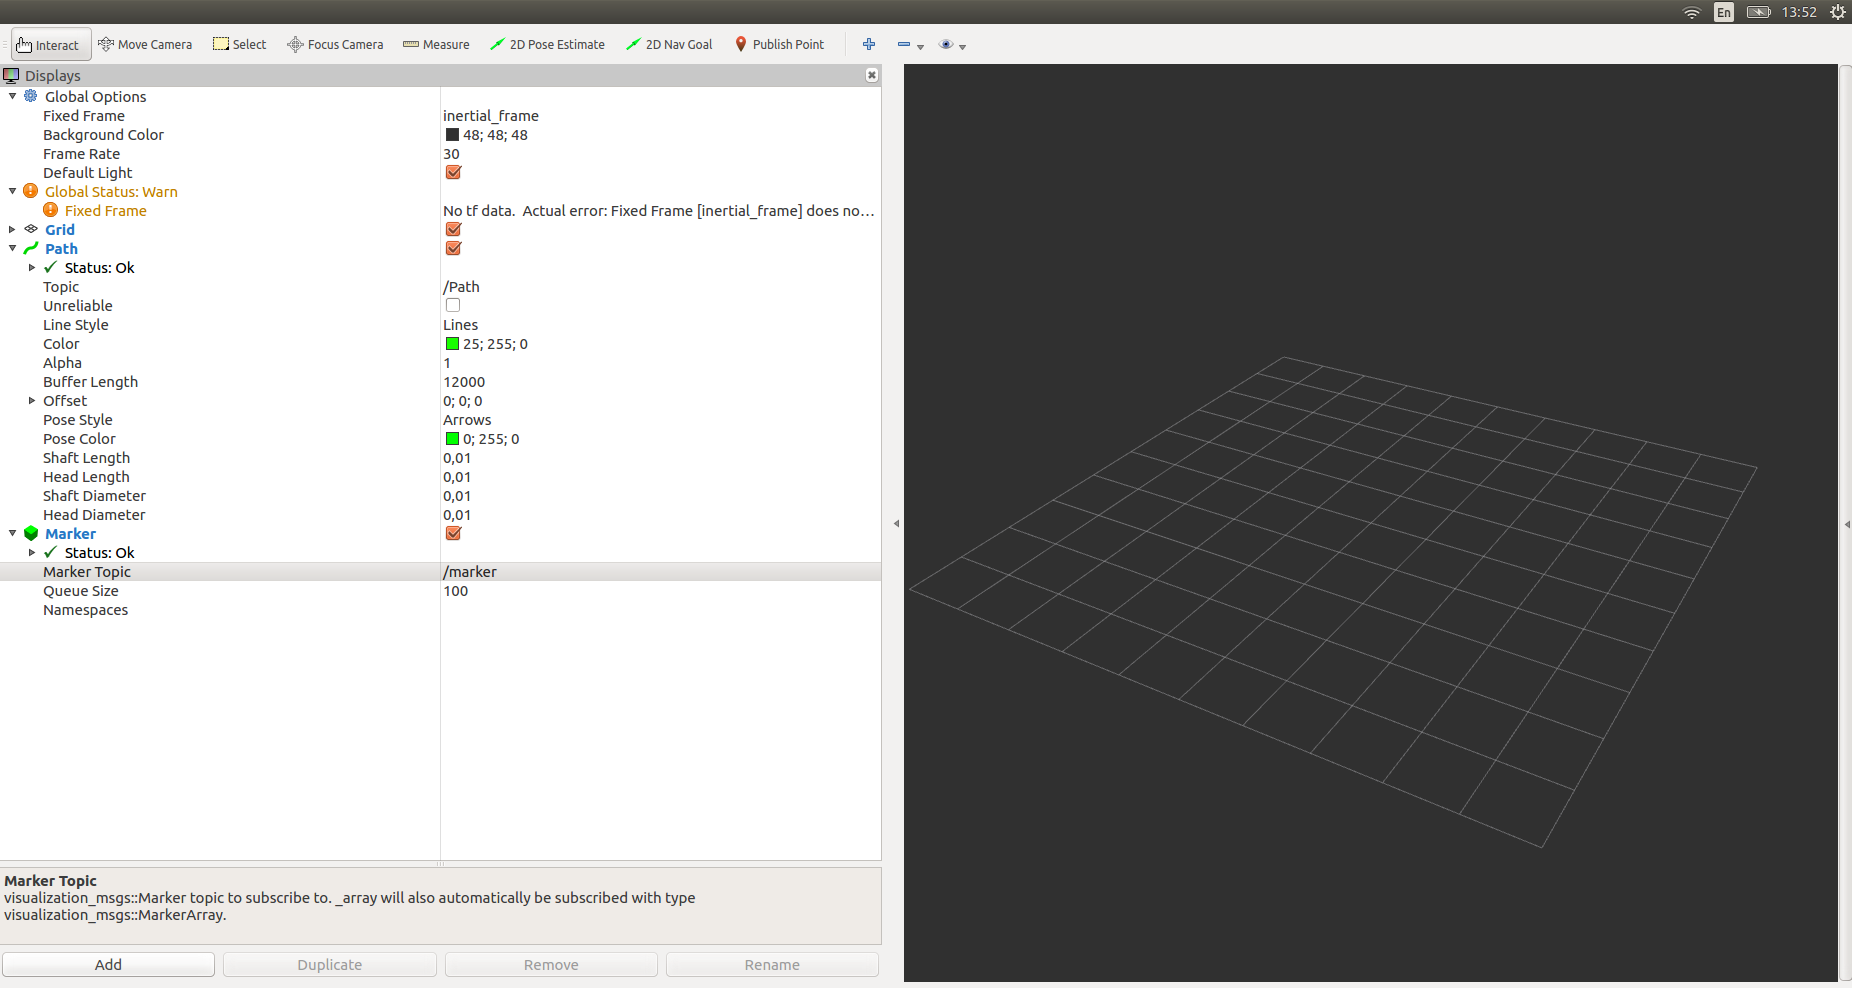
\includegraphics[width=350pt]{figuras/rvizmarker.png}
	\caption{Configuração do Display \textit{/marker}.}
	\label{22}
\end{figure*}

Feito isso o Rviz está configurado e pronto para o uso. Para visualizar a trajetória basta então apertar "step" na simulação configurada no Gazebo de acordo com os exemplos \textbf{VANT 4.0} ou \textbf{VANT 4.0 com Cenário} que a trajetória automaticamente aparecerá no Rviz.

\begin{figure*}[!ht]
	\centering
	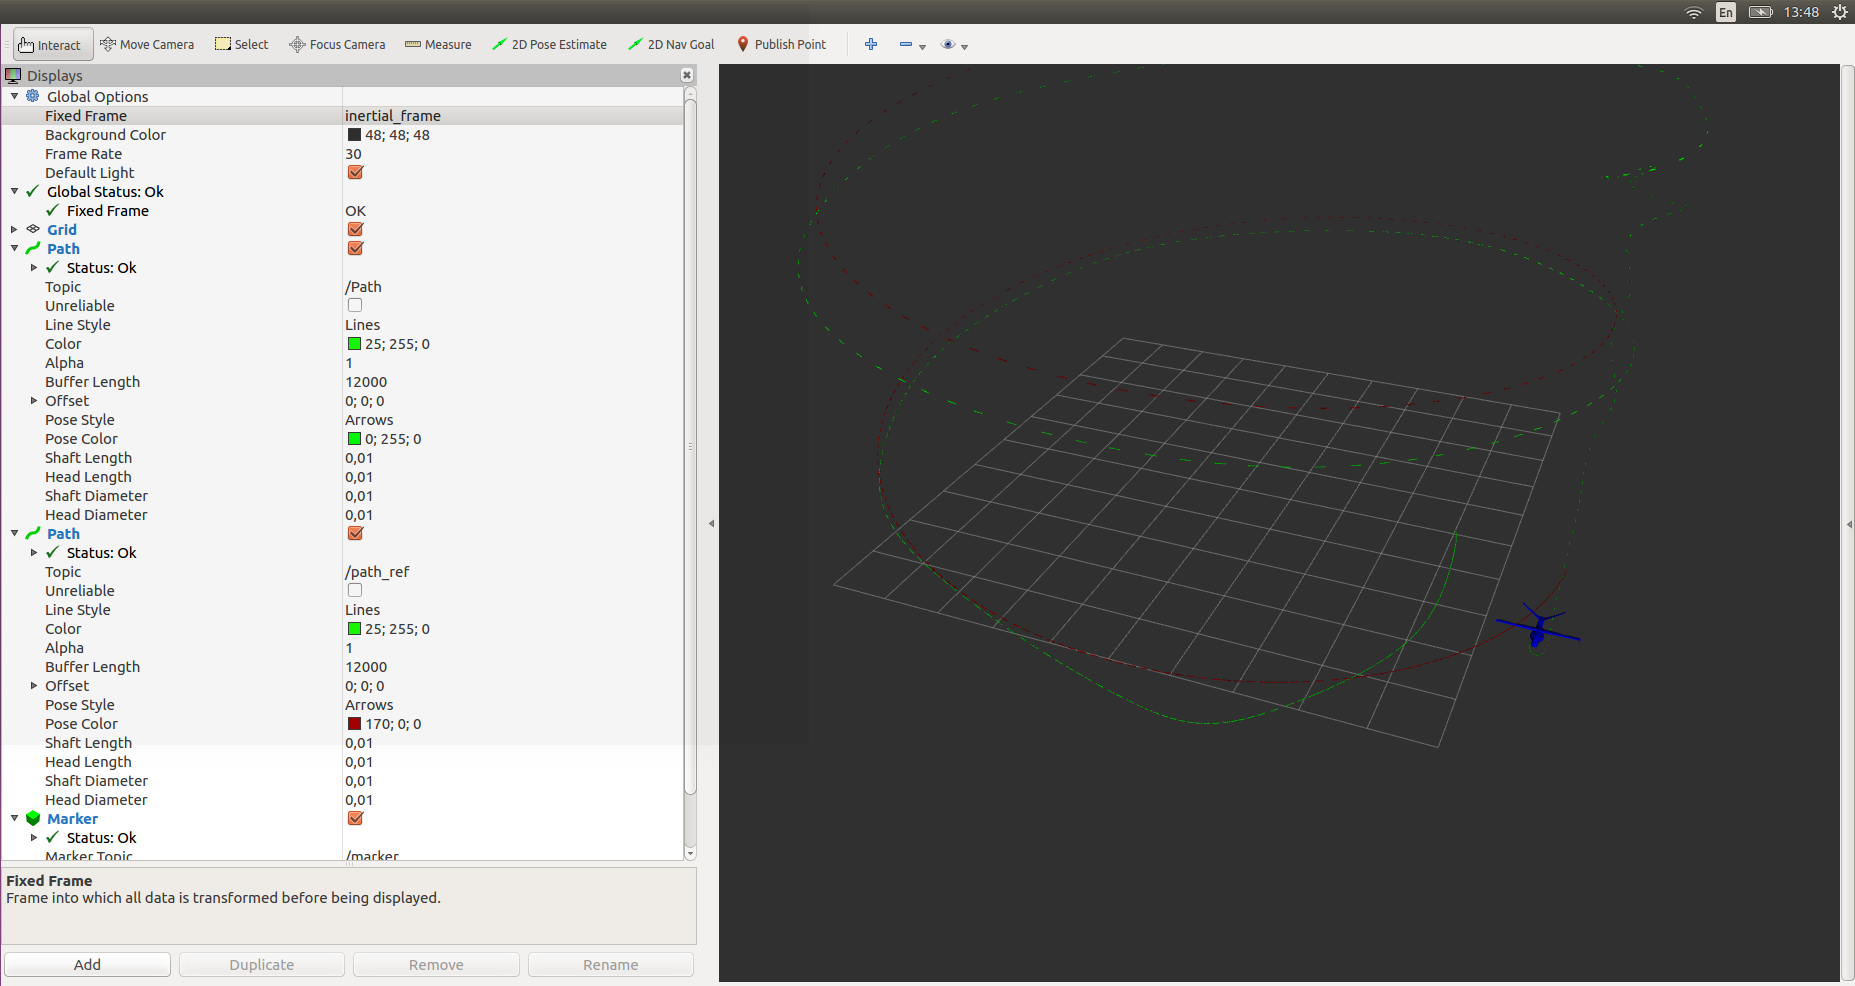
\includegraphics[width=350pt]{figuras/rvizresult.png}
	\caption{Visual da Trajetória no Rviz.}
	\label{23}
\end{figure*}

%--------------------------------------------------------------------


	\subsection{Funcionalidades Extras - Laser Sensor}

Assim como a funcionalidade de câmera tanto o modelo do VANT 4.0 quanto o modelo do Quadrotor possuem a funcionalidade de detecção de obstáculos por meio de um sensor à laser. Os parâmetros que regulam essa funcionalidade estão escritos diretamente no arquivo ".sdf" dos VANTs que pode ser acessado pelo caminho:
\begin{bashcode}	$HOME/catkin_ws/src/ProVANT-Simulator/source/Database/models/vant_4_aerod/robot
	\end{bashcode}
	ou para o Quadrotor
	\begin{bashcode}	$HOME/catkin_ws/src/ProVANT-Simulator/source/Database/models/quadcopter/robot
\end{bashcode}

Ao abrir esses arquivos, logo abaixo da descrição do elo referente ao sensor do laser deverá estar a descrição referente ao sensor que permite detectar obstáculos.

\begin{minted}{xml}
<sensor type="ray" name="laser">
<pose>0 0 0 0 0 0</pose>
<visualize>true</visualize>
<update_rate>30</update_rate>
<ray>
<scan>
<horizontal>
<samples>40</samples>
<resolution>1.0</resolution>
<min_angle>-0.20</min_angle>
<max_angle>0.1</max_angle>
</horizontal>
<vertical>
<samples>40</samples>
<resolution>1.0</resolution>
<min_angle>-0.20</min_angle>
<max_angle>0.1</max_angle>
</vertical>
</scan>
<range>
<min>0.01</min>
<max>2.5</max>
<resolution>0.02</resolution>
</range>
</ray>

<plugin filename="libgazebo_ros_range.so" name="gazebo_ros_range">
<gaussianNoise>0.005</gaussianNoise>
<alwaysOn>true</alwaysOn>
<updateRate>5</updateRate>
<topicName>/sensor/laser</topicName>
<frameName>laser_link</frameName>
<visualize>true</visualize>
<radiation>infrared</radiation>
<fov>0.02</fov>
</plugin>
</sensor>
\end{minted}
Abaixo são listados alguns parâmetros importantes que o usuário pode modificar de acordo com a necessidade.
\begin{itemize}
	\setlength{\itemsep}{1pt}
	\setlength{\parskip}{0pt}
	\setlength{\parsep}{0pt}
	\item[-] \textcolor{blue}{<visualize></visualize>}: define se o laser ficará visível no Gazebo;
	\item[-] \textcolor{blue}{<horizontal></horizontal>}: define parâmetros para feixes de laser na horizontal.  
	\item[-] \textcolor{blue}{<vertical></vertical>}: define parâmetros para feixes de laser na vertical. 
	\item[-] \textcolor{blue}{<samples></samples>}: define o numero de feixes de laser. 
	\item[-] \textcolor{blue}{<resolution></resolution>}:\url{http://sdformat.org/spec?ver=1.6&elem=sensor#horizontal_resolution}. 
	\item[-] \textcolor{blue}{<min\_angle></min\_angle>}: define o ângulo minimo em radianos. 
	\item[-] \textcolor{blue}{<max\_angle></max\_angle>}: define o ângulo máximo em radianos. 
	\item[-] \textcolor{blue}{<range></range>}: define propriedades relacionadas ao alcance de um feixe de laser. 
	\item[-] \textcolor{blue}{<min></min>}: distância mínima de um feixe de laser. 
	\item[-] \textcolor{blue}{<max></max>}: distância mínima de um feixe de laser.
	\item[-] \textcolor{blue}{<topicName></topicName>}: nome do tópico onde os valores das leituras do laser serão publicados.  
\end{itemize}\normalsize

O usuário pode utilizar o comando abaixo para ler os valores do sensor. 
\begin{bashcode}
	rostopic echo /sensor/laser
\end{bashcode}

\begin{figure*}[!ht]
	\centering
	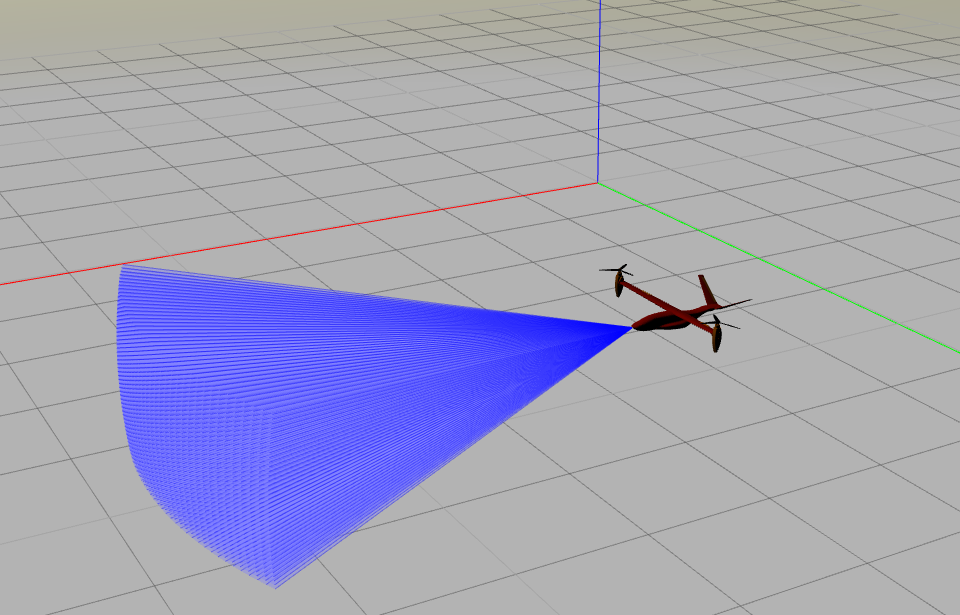
\includegraphics[width=250pt]{figuras/v4laser.png}
	\caption{Laser Sensor no VANT 4.0.}
	\label{v4laser}
\end{figure*}

\begin{figure*}[!ht]
	\centering
	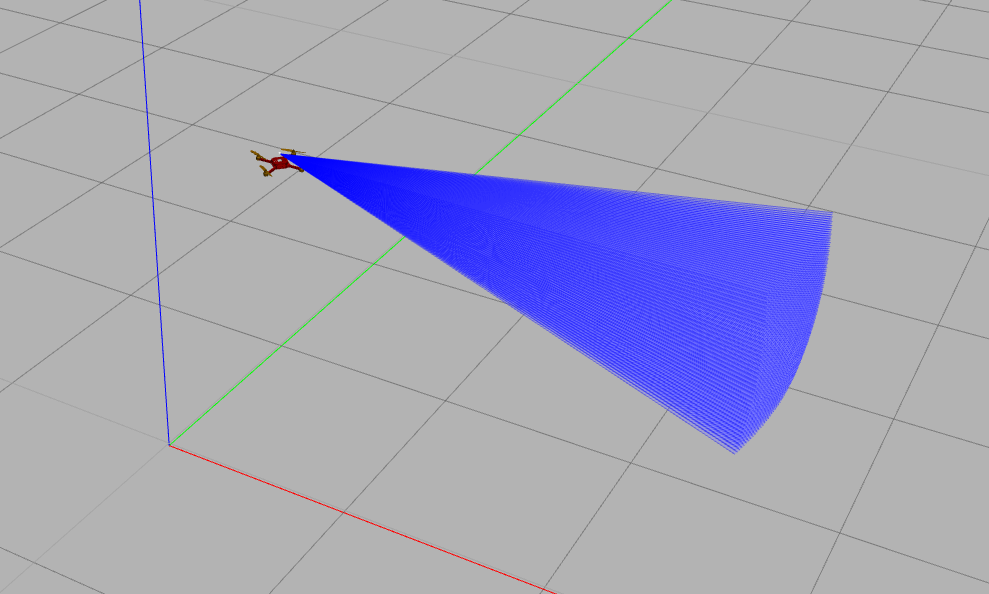
\includegraphics[width=250pt]{figuras/quadlaser.png}
	\caption{Laser Sensor no Quadrotor.}
	\label{quadlaser}
\end{figure*}



%---------------------------------------------------------------------

	\subsection{Funcionalidades Extras - Visão em Primeira Pessoa}
	
Tanto o modelo do VANT 4.0 quanto o modelo do Quadrotor possuem a funcionalidade de permitir ao usuário visualizar a trajetória da perspectiva do VANT. Os parâmetros que regulam essa funcionalidade estão escritos diretamente no arquivo ".sdf" dos VANTs que pode ser acessado pelo caminho:
\begin{bashcode}	$HOME/catkin_ws/src/ProVANT-Simulator/source/Database/models/vant_4_aerod/robot
\end{bashcode}
ou para o Quadrotor
\begin{bashcode}	$HOME/catkin_ws/src/ProVANT-Simulator/source/Database/models/quadcopter/robot
\end{bashcode}
Ao abrir esses arquivos, logo abaixo da descrição do elo referente à câmera deverá estar a descrição referente ao sensor que permite as funções de câmera.
\begin{minted}{xml}
<sensor name="camera" type="depth">
	<camera>
		<horizontal_fov>1.047</horizontal_fov>
			<image>
				<width>320</width>
				<height>240</height>
			</image>
		<clip>
			<near>0.1</near>
			<far>100</far>
		</clip>
	</camera>
	<always_on>1</always_on>
	<update_rate>30</update_rate>
	<visualize>true</visualize>
<plugin name="camera_plugin" filename="libgazebo_ros_openni_kinect.so">
	<baseline>0.2</baseline>
	<alwaysOn>true</alwaysOn>
<!-- Keep this zero, update_rate in the parent <sensor> tag
will control the frame rate. -->
	<updateRate>0.0</updateRate>
	<cameraName>camera_ir</cameraName>
	<imageTopicName>/camera/color/image_raw</imageTopicName>
	<cameraInfoTopicName>/camera/color/camera_info</cameraInfoTopicName>
	<depthImageTopicName>/camera/depth/image_raw</depthImageTopicName>
	<depthImageCameraInfoTopicName>/camera/depth/camera_info</depthImageCameraInfoTopicName>
	<pointCloudTopicName>/camera/depth/points</pointCloudTopicName>
	<frameName>camera_link</frameName>
	<pointCloudCutoff>0.5</pointCloudCutoff>
	<pointCloudCutoffMax>3.0</pointCloudCutoffMax>
	<distortionK1>0</distortionK1>
	<distortionK2>0</distortionK2>
	<distortionK3>0</distortionK3>
	<distortionT1>0</distortionT1>
	<distortionT2>0</distortionT2>
	<CxPrime>0</CxPrime>
	<Cx>0</Cx>
	<Cy>0</Cy>
	<focalLength>0</focalLength>
	<hackBaseline>0</hackBaseline>
</plugin>
</sensor>
\end{minted}
\centerline{Código: Funcionalidade "Câmera" no arquivo model.sdf}

A funcionalidade desse sensor é bastante ampla podendo funcionar como uma câmera normal ou também como uma \textit{depth camera} onde é possivel vizualizar no rviz objetos identificados utilizando o display \textit{PointCloud2}.
Inicializando o Rviz deve-se primeiro alterar no menu de displays a opção \textit{Fixed Frame}, responsável por definir o sistema de coordenadas com que os parâmetros dos diversos \textit{displays} operam, para o sistema de coordenadas da câmera definido na \textit{tag} \textcolor{blue}{<frameName></frameName>}, "camera\_link",então adicionar o \textit{display} de Câmera.

\begin{figure*}[!ht]
	\centering
	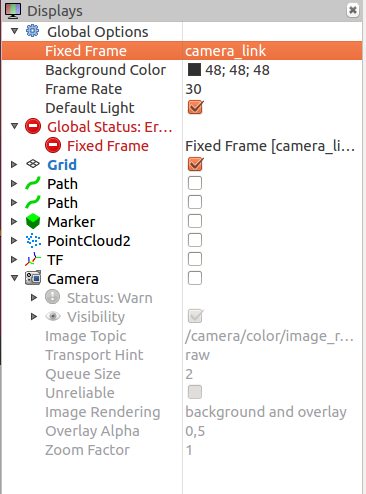
\includegraphics[width=150pt]{figuras/camrviz.png}
	\caption{Configuração do \textit{Display} Câmera}
	\label{camrviz}
\end{figure*}

Caso não seja preenchido automaticamente, o parâmetro tópico deverá ser preenchido com o nome do tópico definido no arquivo ".sdf" na \textit{tag} \textcolor{blue}{<imageTopicName></imageTopicName>}
Ao inicializar uma simulação com o VANT 4.0 ou com o Quadrotor será possível visualizar a trajetória feita sob a perpectiva do VANT.

\begin{figure*}[!ht]
	\centering
	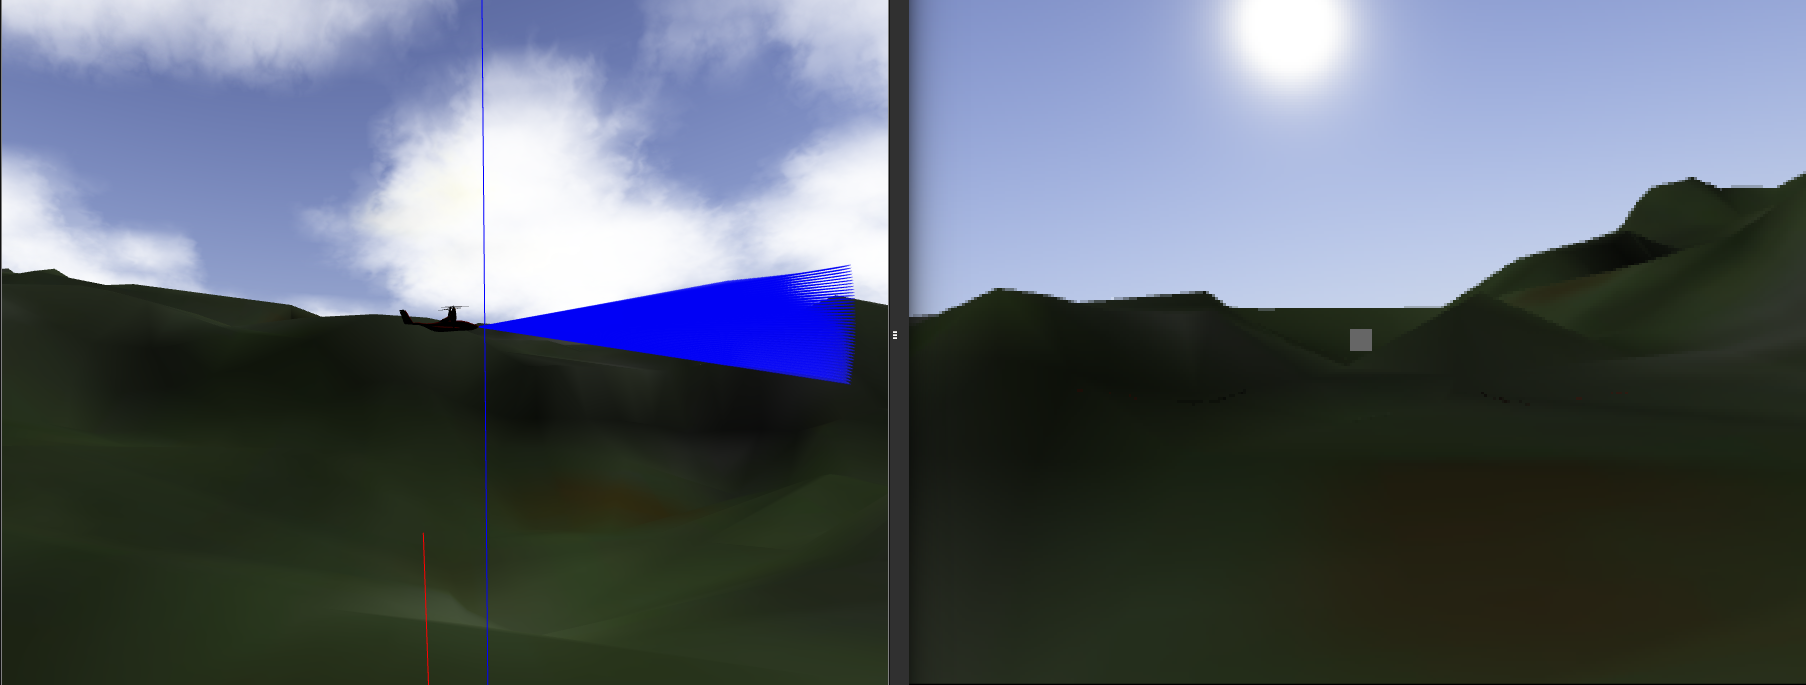
\includegraphics[width=450pt]{figuras/camerav4.png}
	\caption{Visão em Primeira Pessoa VANT 4.0.}
	\label{v4camera}
\end{figure*}

\begin{figure*}[!ht]
	\centering
	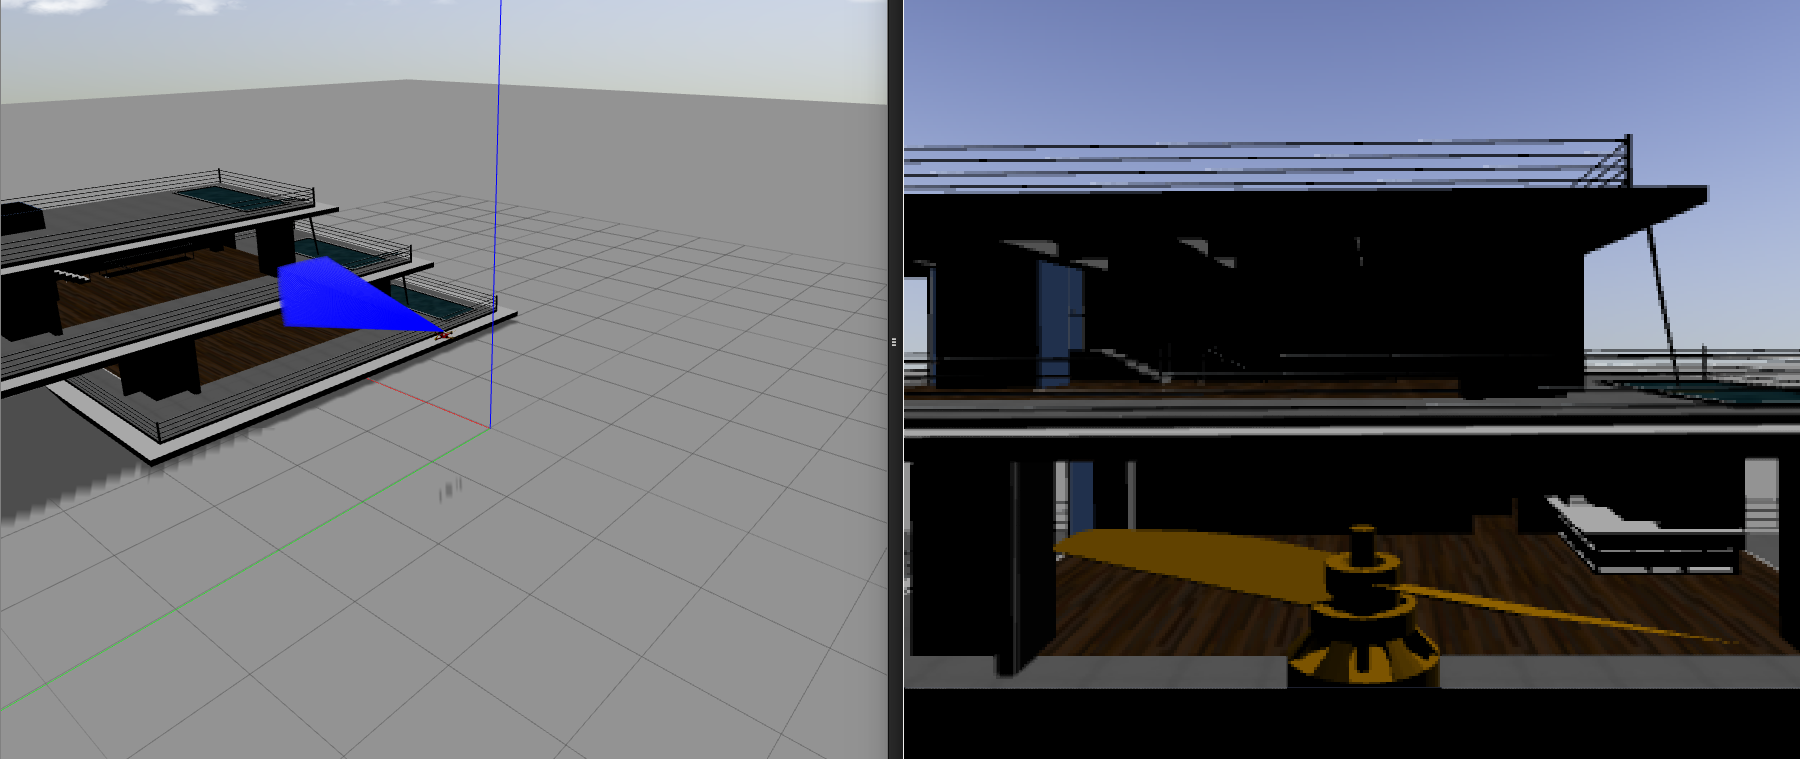
\includegraphics[width=450pt]{figuras/quadcam.png}
	\caption{Visão em Primeira Pessoa Quadrotor.}
	\label{quadamera}
\end{figure*}


%------------------------------------------------------------------------------------%
\chapter{Projeto de estratégia de controle}
\label{controle}

Neste capítulo são detalhados os procedimentos necessários para implementação de estratégias de controle no ambiente de simulação. Inicialmente é descrita a organização e a estrutura dos arquivos necessários para implementação da estratégia de controle. Por fim, apresenta-se o processo de criação de uma nova estratégia de controle com a finalidade de ilustrar o procedimento apresentado na Seção \ref{SecEstCtrl}.

\section{Organização}

%O espaço de trabalho do ROS é organizado em módulos de software denominados "Pacotes". O ambiente de simulação, por sua vez, aproveita dessa organização para sistematizar o projeto de estratégia de controle, pois cada projeto é considerado um pacote. 

De modo geral a estrutura de arquivos do projeto de controle está organizada como illustrado na Figura \ref{pacote}:%, deve possuir os seguintes diretórios e arquivos: \\

\begin{figure}[H]
	\center
	\begin{tikzpicture}[%
	grow via three points={one child at (0.5,-0.7) and
		two children at (0.5,-0.7) and (0.5,-1.4)},
	edge from parent path={(\tikzparentnode.south) |- (\tikzchildnode.west)}]
	\node {Name\_of\_control\_Strategy/}
	child { node {src/}
		child { node {main.cpp}}
	}
	child [missing] {}
	child { node {include/}}		
	child { node {CMakeLists.txt}}
	child { node {package.xml}};
	\end{tikzpicture}
	\caption{Organização do diretório de projeto de estratégias de controle. Os diretórios são dados pelas ''caixinhas'' com nomes terminados pelo caractere ''/'' e os arquivos possuem alguma extensão em seu nome.}
	\label{pacote}
\end{figure}


%\noindent
%Obs.: Os diretórios são dados pelas ''caixinhas'' com nomes terminados pelo caractere ''/'', e os arquivos possuem alguma extensão em seu nome.


\begin{itemize}
	\itemsep0em 
	\item[-]O arquivo ''main.cpp'' é o arquivo onde é implementada a lógica da estratégia de controle.
	\item[-]A pasta ''include'' armazena bibliotecas customizadas pelo usuário que são incluídas no preâmbulo do arquivo main.cpp.
	\item[-]O arquivo ''CMakeLists.txt'' fornece ao compilador informações sobre o diretório de bibliotecas incluídas nos códigos fontes do simulador. Detalhes sobre como incluir novas bibliotecas podem ser encontrados no Apêndice \ref{cmake}.
	\item[-]O arquivo ''package.xml'' é o arquivo necessário para armazenar dados como nome do autor, endereço de e-mail, etc. Detalhes de sua configuração são apresentados no Apêndice \ref{package}.
\end{itemize}



\section{Interface padrão para desenvolvimento de estratégias de controle e template main.cpp}

A criação de uma estratégia de controle é realizada através de herança da classe virtual padrão "IController". Sendo essa uma classe virtual, seus métodos precisam ser implementadas na classe filha. A Figura \ref{interface} ilustra suas funções métodos. 

A função método  \textit{config()} é executada no inicio das simulações, sendo utilizada para realizar configurações iniciais da estratégia de controle. O método \textit{execute()} é chamado pelo simulador a cada período de amostragem. Ele é \textbf{o método que deve conter toda a lógica da estratégia de controle}. A ordem e quantidade dos sinais entrada e saída desta função é determinada na interface como descrito na subseção \ref{sensoresatuadores}. As funções \textit{state()}, \textit{error()} e \textit{reference()} são métodos que retornam os valores dos sinais de erro, referência e sensores para serem armazenados em arquivos de texto. Os dados salvos nos arquivos txt podem ser utilizado para produzir gráficos dos resultados da simulação, utilizando o matlab, por exemplo. 



%A estratégia de controle deve ser implementada através de uma classe que herda uma interface padrão de comunicação com o ambiente de simulação, chamada IController, que está ilustrada na Figura \ref{interface}.

\begin{figure}[!ht]
\begin{minted}{cpp}
#ifndef ICONTROLLER_HPP
#define ICONTROLLER_HPP

#include "simulator_msgs/SensorArray.h"

class Icontroller 
{
	public:
	Icontroller(){};
	virtual ~Icontroller(){};
	virtual void config()=0;
	virtual std::vector<double> execute(simulator_msgs::SensorArray)=0;
	virtual std::vector<double> Reference()=0;
	virtual std::vector<double> Error()=0;
	virtual std::vector<double> State()=0;
};

extern "C" {
	typedef Icontroller* create_t();
	typedef void destroy_t(Icontroller*);
}
#endif
\end{minted}
\caption{Interface de implementação de estratégias de controle.}
\label{interface}
\end{figure}

%Esta interface orienta ao usuário os métodos virtuais necessários de se implementar. 

Quando uma nova estratégia de controle é criada, o ambiente de simulação fornece um arquivo main.cpp como template básico para a implementação da estratégia de controle. O conteúdo deste arquivo está ilustrado na Figura \ref{template}. A próxima seção apresenta um exemplo de implementação de estratégia de controle.

\begin{figure}[!ht]
\begin{minted}{cpp}
#include "Icontroller.hpp"

class demonstracao : public Icontroller
{
	public: demonstracao(){}
	public: ~demonstracao(){}
	public: void config(){}
	public: std::vector<double> execute(simulator_msgs::SensorArray arraymsg)
	{
		std::vector<double> out;
		return out;
	}
	public: std::vector<double> Reference()
	{
		std::vector<double> out;
		return out;
	}
	public: std::vector<double> Error()
	{
		std::vector<double> out;
		return out;
	}
	public: std::vector<double> State()
	{
		std::vector<double> out;
		return out;
	}
};

extern "C"
{
	Icontroller *create(void) {return new demonstracao;}
	void destroy(Icontroller *p) {delete p;}
}
\end{minted}
\caption{Template para implementação de estratégias de controle.}
\label{template}
\end{figure} 

\section{Exemplo de implementação de estratégia de controle}
\label{exemplo}

Esta seção demonstra o processo de implementação de uma nova estratégia de controle. Nela é apresentado um exemplo de utilização da interface gráfica para a criação e modificação de uma nova estratégia de controle, e também o processo de compilação. O exemplo utilizado corresponde à implementação de uma estratégia de controle robusto para rastreamento de trajetória da carga, transportada por um VANT na configuração Tilt-rotor. Mais detalhes da estratégia de controle pode ser encontrados em \cite{Lara2017}.


\subsection{Configurando a lista de sensores e atuadores disponíveis}

Na janela descrita na Seção \ref{SecEstCtrl}, ao selecionar a aba Sensors ou Actuator, uma das janelas illustrada na Figura \ref{abas} aparecerá. Em ambas, o usuário pode adicionar e remover instrumentos da lista utilizando os botões ''Add'' e ''Remove''. Além disso, clicando duas vezes sobre um nome na lista, é possível editar as propriedades do instrumento. Estas listas são de fundamental importância para a implementação da estratégia de controle, tais instrumentos e sua respectiva ordem definirão os dados de entrada e saída do controlador.

\begin{figure}[h!]
	\hfill
	\subfloat{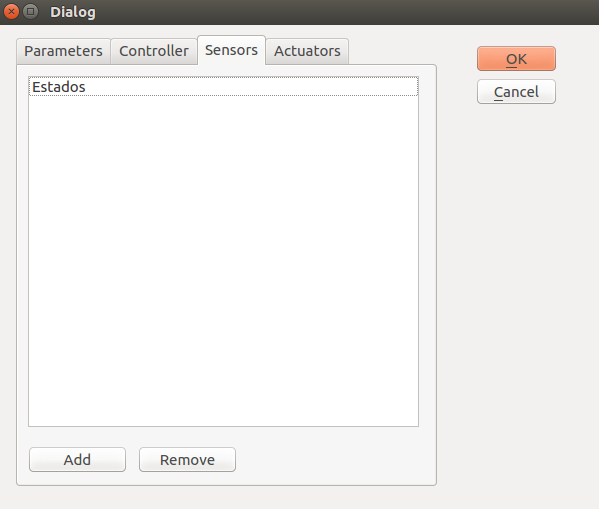
\includegraphics[width=230pt]{figuras/6.png}}
	\hfill
	\subfloat{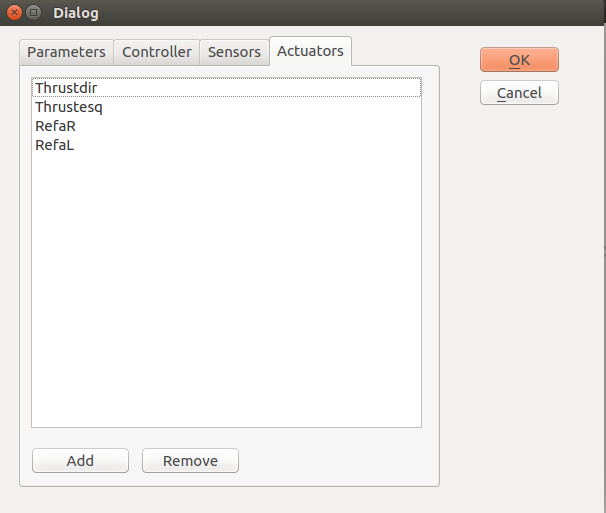
\includegraphics[width=230pt]{figuras/7.png}}
	\hfill
	\caption{Abas Sensors e Actuators.}
	\label{abas}
\end{figure}

Neste exemplo, o controlador receberá um vetor de sensores, no entanto contendo informações fornecidas por um único sensor, cujo tópico de comunicação é denominado ''Estados''. Além disso, o controlador deverá  retornar um vetor de ponto flutuante de dimensão 4 com sinais de entrada de controle para atuadores, cujos tópicos de comunicação estão na seguinte ordem: 1) Thrustdir, 2) Thrustesq, 3) RefaR e 4) RefaL.

\subsection{Criando uma nova estratégia de controle}

Para criar uma nova estratégia de controle, na aba Controller, pressione ''New Controller''. Uma nova janela será mostrada solicitando ao usuário o nome do novo controlador. Neste exemplo, a estratégia de controle terá o nome ''vant2load\_hinfinity'' (Figura \ref{projeto1}). Depois de confirmar o nome do controlador, uma janela do Nautilus aparecerá com o diretório do projeto criado (Figura \ref{2a}).

\begin{figure*}[!ht]
	\centering
	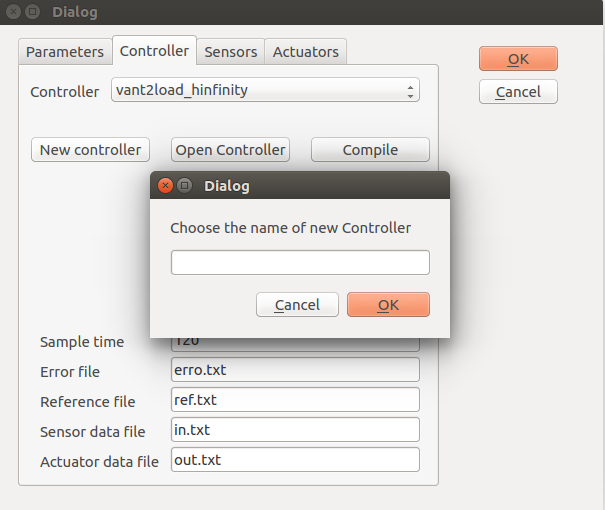
\includegraphics[width=0.7\columnwidth]{figuras/1a1a1.png}
	\caption{Criando uma nova estratégia de controle.}
	\label{projeto1}
\end{figure*}

\begin{figure*}[!ht]
	\centering
	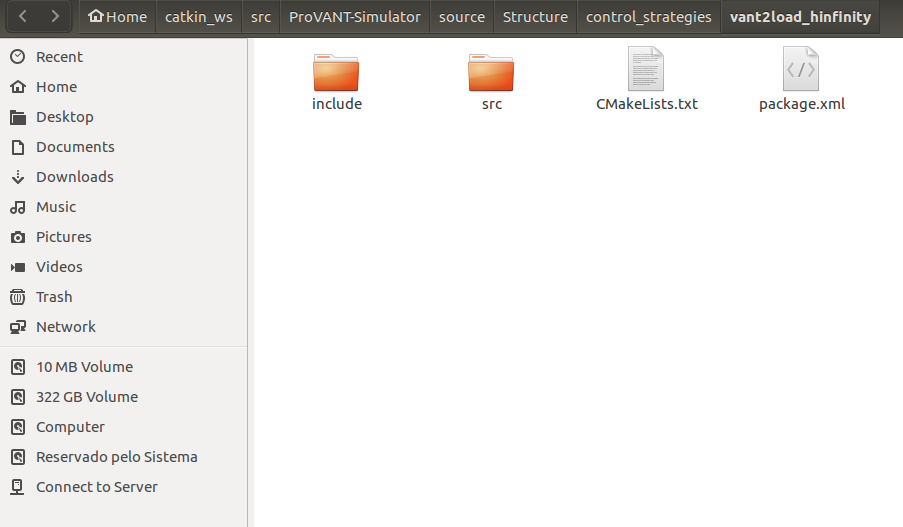
\includegraphics[width=0.7\columnwidth]{figuras/2a.png}
	\caption{Arquivos e diretórios associados à nova estratégia de controle.}
	\label{2a}
\end{figure*}

\subsection{Implementação da estratégia de controle}

A Figura \ref{exemplo1} mostra um exemplo de código de estratégia de controle implementada no arquivo main.cpp. No exemplo, observa-se que é necessário a inclusão de 3 bibliotecas: 

\begin{figure}
\begin{minted}{cpp}
#include "Icontroller.hpp"
#include <Eigen/Eigen>
#include "simulator_msgs/Sensor.h"
	
class hinfinity : public Icontroller 
{
	private: Eigen::VectorXd Xref; // vetor de referência
	private: Eigen::VectorXd Erro; // vetor de erros
	private: Eigen::VectorXd Input; // sinais de controle
	private: Eigen::MatrixXd K; // matriz de ganhos do controlador
	private: Eigen::VectorXd X; // vetor de estados
	private: double T; // Período de amostragem
	
	public: hinfinity(): Xref(24), K(4,24), X(24), Erro(24), Input(4)
	{ 
		T = 0.012;
	}
	public: ~hinfinity(){	}
	
	public: void config()
	{	
		K<< [...] Dados da matriz [...];
	}
	public: std::vector<double> execute(simulator_msgs::SensorArray arraymsg)
	{
		static float count = 0;
		static float xint, x_ant = 0;
		static float yint, y_ant = 0;
		static float zint, z_ant = 0;
		static float yawint, yaw_ant = 0;
		// selecionando dados
		int i = 0;		
		simulator_msgs::Sensor msgstates;
		msgstates = arraymsg.values.at(0);		
		// Referência
		float trajectoryRadius = 2;
		float trajectoryHeight = 4*trajectoryRadius;
		float trajTime = 80;
		float pi = 3.14;
		float x = trajectoryRadius*cos((count*T)*2*pi/trajTime);
		float xdot = -trajectoryRadius*(2*pi/trajTime)*sin((count*T)*2*pi/trajTime);
		float xddot = -trajectoryRadius*(2*pi/trajTime)*(2*pi/trajTime)
				*cos((count*T)*2*pi/trajTime);
		float y = trajectoryRadius*sin((count*T)*2*pi/trajTime);
		float ydot = trajectoryRadius*(2*pi/trajTime)*cos((count*T)*2*pi/trajTime);
		float yddot = -trajectoryRadius*(2*pi/trajTime)*(2*pi/trajTime)
				*sin((count*T)*2*pi/trajTime);
		float z = trajectoryHeight+1 - trajectoryHeight*cos((count*T)*2*pi/trajTime);
		float zdot = trajectoryHeight*(2*pi/trajTime)*sin((count*T)*2*pi/trajTime);
		float zddot = trajectoryHeight*(2*pi/trajTime)*(2*pi/trajTime)
				*cos((count*T)*2*pi/trajTime);
		Xref << x,y,z,0,0,0,0.00002965,0.004885,0.004893,0.00484,xdot,ydot,zdot,
			0,0,0,0,0,0,0,0,0,0,0;
		
		\end{minted}
		\end{figure}
		\begin{figure}
		\begin{minted}{cpp}
		//Convertendo velocidade angular
		std::vector<double> etadot = pqr2EtaDot(msgstates.values.at(13),
		msgstates.values.at(14),
		msgstates.values.at(15),
		msgstates.values.at(3),
		msgstates.values.at(4),
		msgstates.values.at(5));
		
		// Integrador Trapezoidal
		float x_atual = msgstates.values.at(0) - Xref(0);
		xint = xint + (T/2)*(x_atual + x_ant);
		x_ant = x_atual;
		float y_atual = msgstates.values.at(1) - Xref(1);
		yint = yint + (T/2)*(y_atual + y_ant);
		y_ant = y_atual;
		float z_atual = msgstates.values.at(2) - Xref(2);
		zint = zint + (T/2)*(z_atual + z_ant);
		z_ant = z_atual;
		float yaw_atual = msgstates.values.at(5) - Xref(5);
		yawint = yawint + (T/2)*(yaw_atual + yaw_ant);
		yaw_ant = yaw_atual;
		
		// vetor de estados aumentado
		X << msgstates.values.at(0),//x
		msgstates.values.at(1),//y
		msgstates.values.at(2),//z
		msgstates.values.at(3),//roll
		msgstates.values.at(4),//pitch
		msgstates.values.at(5),//yaw
		msgstates.values.at(8),//g1 x
		msgstates.values.at(9),//g2 y
		msgstates.values.at(6),//aR
		msgstates.values.at(7),//aL
		msgstates.values.at(10),//vx
		msgstates.values.at(11),//vy
		msgstates.values.at(12),//vz
		etadot.at(0),//droll
		etadot.at(1),//dpitch
		etadot.at(2),//dyaw
		msgstates.values.at(18), // angulo da primeira junta da carga
		msgstates.values.at(19), // angulo da segunda junta da carga
		msgstates.values.at(16), // derivada do angulo da primeira junta da carga
		msgstates.values.at(17), // derivada do angulo da segunda junta da carga
		xint,
		yint,
		zint,
		yawint;
		
		
		// lei de controle
		Erro = X-Xref;
		Input = -K*Erro;
		
		\end{minted}
		\end{figure}
		\begin{figure}
		\begin{minted}{cpp}
		
		// Criando vetor com dados da trajetória de referência
		Eigen::MatrixXd qref(10,1);
		qref << x,y,z,0,0,0,0.00002965,0.004885,0.004893,0.00484;
		Eigen::MatrixXd qrefdot(10,1);
		qrefdot << xdot,ydot,zdot,0,0,0,0,0,0,0;
		Eigen::MatrixXd qrefddot(10,1);
		qrefddot << xddot,yddot,zddot,0,0,0,0,0,0,0;
		
		// Feedforward
		Input(0) = Input(0) + 12.6005;
		Input(1) = Input(1) + 12.609;
		count++; 
		
		
		// convertendo dados do vetor da biblioteca Eigen para vetor a biblioteca padrão de C++
		std::vector<float> out2(Input.data(), Input.data() + Input.rows() 
					* Input.cols());
		
		std::vector<double> out(out2.size());
		for(int i=0; i<out2.size();i++) out.at(i) = out2.at(i);
		return out;
	}
	
	public: std::vector<double> Reference()
	{
		std::vector<double> out(Xref.data(), Xref.data() + Xref.rows() 
					* Xref.cols());
		return out;
	}
	
	public: std::vector<double> Error()
	{
		std::vector<double> out(Erro.data(), Erro.data() + Erro.rows() 
					* Erro.cols());	
		return out;
	}	
	
	public: std::vector<double> State()
	{
		std::vector<double> out(X.data(), X.data() + X.rows() * X.cols());
		return out;
	}
	
	private: std::vector<double> pqr2EtaDot(double in_a, double in_b, double in_c, 
						double phi, double theta, double psii)
	{
		std::vector<double> out;
		out.push_back(in_a + in_c*cos(phi)*tan(theta) + in_b*sin(phi)*tan(theta));
		out.push_back(in_b*cos(phi) - in_c*sin(phi));
		out.push_back((in_c*cos(phi))/cos(theta) + (in_b*sin(phi))/cos(theta));
		return out;
	}
};
	
	\end{minted}
	\end{figure}
	\begin{figure}
	\begin{minted}{cpp}
	
extern "C"
{ 
	Icontroller *create(void) {
		return new hinfinity;
	}
	void destroy(Icontroller *p) {
		delete p;
	}
}
\end{minted}
\caption{Exemplo de código.}
\label{exemplo1}
\end{figure}

\begin{itemize}
		\setlength{\itemsep}{1pt}
		\setlength{\parskip}{0pt}
		\setlength{\parsep}{0pt}
\item \#include ''Icontroller.hpp''  - informa ao código a interface padrão para criação de controladores no ambiente de simulação;
\item \#include <Eigen/Eigen> - importa as funcionalidades fornecidas pela biblioteca Eigen \footnote{https://eigen.tuxfamily.org}. A biblioteca Eigen fornecer funções para realizar operações da álgebra linear;
\item \#include ''simulator\_msgs/Sensor.h'' - informa a classe responsável por abstrair o padrão de comunicação entre o controlador e os sensores.
\end{itemize}


Os atributos \textbf{Xref}, \textbf{Erro}, \textbf{Input}, \textbf{K} e \textbf{X} são as estruturas de de vetores e matrizes da biblioteca Eigen. Essas estruturas são responsáveis por realizar a operações de álgebra linear e, portanto, permitir a relização da lei de controle. O atributo \textbf{T} determina o período de amostragem do controlador.

O construtor hinfinity() inicializa os atributos da classe, enquanto o destrutor \textasciitilde hinfinity() não possui nenhuma função no contexto do simulador.

Neste exemplo, o método config() é utilizado para atribuir valores à matriz de ganhos K, respeitando a sintaxe da biblioteca Eigen, no entanto o usuário pode utilizar esse espaço para realizar qualquer outra configuração inicial. Por fim, a lógica da estratégia de controle é implementada no método execute(), que é executado a cada período de amostragem, como descrito anteriormente.

O código começa por declarar as variáveis (estáticas) ''xint'', ''x\_ant'', ''yint'', ''y\_ant'', ''zint'', ''z\_ant'', ''yawint'' e ''yaw\_ant'', utilizadas para armazenar os valores dos integradores implementados na estratégia de controle. Em seguida, está presente o trecho de código referente aos dados dos sensores, obtidos através do vetor ''arraymsg''. Como neste exemplo somente um sensor está disponível (''Estados''), apenas a primeira posição deste vetor é acessada (através da sintaxe ''arraymsg.values.at(0)''). Nos casos em que mais sensores são disponibilizados, os dados do n-ésimo sensor são acessados através de  ''arraymsg.values.at(n-1)'' e a ordem desse vetor é definida a priori na aba Sensor conforme é visualizada em \ref{6}. Em seguida, é definido a referência para o controlador e implementado integradores, através do método de integração trapezoidal, para realização da lei de controle e, por fim, é calculada a ação de controle feedforward. 

Os métodos Reference(), Error(), State() são utilizados para armazenar dos sinais de referência, erro e estados, respectivamente, nos arquivos de texto de saída do ambiente de simulação. A função pqr2EtaDot() corresponde a um mapeamento de parte das informações recebidas pelos sensores, necessário para a implementação da estratégia de controle deste exemplo. 

Assim como a função pqr2EtaDot(), quaisquer funções adicionais que sejam necessárias para a implementação da estratégia de controle, podendo estar relacionadas também a algoritmos de filtragem, podem ser escritas dentro da classe ''main.cpp'', ou em classes auxiliares criadas dentro da pasta ''include'' ilustrada em \ref{2a} (neste caso, estas devem ser também incluídas no cabeçalho do arquivo ''main.cpp'').


Por fim, o trecho de código a seguir corresponde à funções necessárias para garantir o carregamento da estratégia de controle em tempo de execução do simulador. O método create() cria uma instância da classe que encapsula o controlador, e o método destroy() é utilizado para destruir a instância da classe.

\begin{minted}{cpp}
extern "C"
{ 
	Icontroller *create(void) {
		return new hinfinity;
	}
	void destroy(Icontroller *p) {
		delete p;
	}
}
\end{minted}


%\subsection{Configurando CMakeLists.txt}
%
%Em seguida, substitua o código template do CMakeLists.txt com o seguinte código.
%
%
%\begin{minted}{xml}
%cmake_minimum_required(VERSION 2.8.3)
%project(vant2load_hinfinity)
%
%find_package(catkin REQUIRED COMPONENTS
%			roscpp
%			simulator_msgs)
%	
%include_directories(include)
%INCLUDE_DIRECTORIES (/usr/include/eigen3)
%include_directories( ${catkin_INCLUDE_DIRS})
%include_directories($ENV{TILT_PROJECT}/source/Structure/control_strategies/)
%
%add_library(vant2load_hinfinity src/hinfinity.cpp)
%target_link_libraries(vant2load_hinfinity ${catkin_LIBRARIES})
%install(TARGETS
%vant2load_hinfinity
%ARCHIVE DESTINATION ${CATKIN_PACKAGE_LIB_DESTINATION}
%LIBRARY DESTINATION ${CATKIN_PACKAGE_LIB_DESTINATION}
%RUNTIME DESTINATION ${CATKIN_PACKAGE_BIN_DESTINATION})
%\end{minted}
%
%
%\subsection{Configurando package.xml}
%
%Em seguida, substitua o código template do package.xml com o seguinte código.
%
%\begin{minted}{xml}
%<?xml version="1.0"?>
%<package>
%	<name>vant2load_hinfinity</name>
%	<version>1.0.0</version>
%	<description>The hinfinity package</description>
%	
%	<maintainer email="macro@todo.todo">macro</maintainer>
%	<license>TODO</license>
%	
%	<buildtool_depend>catkin</buildtool_depend>
%	<build_depend>roscpp</build_depend>
%	<run_depend>roscpp</run_depend>
%	<build_depend>simulator_msgs</build_depend>
%	<run_depend>simulator_msgs</run_depend>
%	
%	<export>
%	</export>
%
%</package>
%\end{minted}
%
%O arquivo package.xml deste exemplo informa que o nome do pacote que encapsula o projeto de controle é denominada de "vant2load_hinfinity"

\subsection{Compilando o código da estratégia de controle}

Após a implementação da estratégia de controle, o código correspondente pode ser compilado através do botão ''Compile'' (conforme explicado no Capítulo 2, vide Figura \ref{5}, item 4).

%\chapter{Inserção de novo cenário}
%
%Um cenário no Gazebo é uma instância de simulação composto por um ou mais modelos incluídos. Este ambiente de simulação está formatado para o funcionamento de apenas um VANT, sendo que demais modelos incluídos são ilustrativos. Há duas maneiras de se incluir um novo cenário: cenário template e cenário editável e pronto para simular. 
%
%O cenário template é a criação de um arquivo com sufixo ".tpl" que tenha apenas elementos ilustrativos e não seja editável pela interface gráfica de configuração. Já o outro é um cenário pronto para uso com VANT definido com sufixo ".world". A estrutura organizacional de ambos os cenários está ilustrado a seguir:
%
%
%\begin{lstlisting}
%<?xml version="1.0" encoding="UTF-8"?>
%<sdf version="1.6">
%	<world name="/home/macro/catkin_ws/src/provant_simulator/source/Database/simulation_elements/worlds/templates/empty/empty2.tpl">
%		<gravity>0.000000 0.000000 -9.8000</gravity>
%		<physics type="ode">
%			<max_step_size>0.001000</max_step_size>
%			<real_time_factor>0</real_time_factor>
%		</physics>
%		<plugin name="gazebo_tutorials" filename="libgazebo_ros_world_plugin.so"/>
%		<include>
%			<uri>model://ground_plane</uri>
%			<static>false</static>
%		</include>
%		<include>
%			<uri>model://sun</uri>
%			<static>false</static>
%		</include>
%		<include>
%			<uri>model://vant_2.0</uri>
%			<name>newmodel</name>
%			<static>false</static>
%			<pose>0 0 2 0 0 0</pose>
%		</include>
%		<scene>
%			<sky>
%				<time>18</time>
%				<clouds>
%					<speed>0</speed>
%				</clouds>
%			</sky>
%		</scene>
%	</world>
%</sdf>
%\end{lstlisting}
%
%onde,
%
%\begin{itemize}
%	\setlength{\itemsep}{1pt}
%	\setlength{\parskip}{0pt}
%	\setlength{\parsep}{0pt}
%	\item[-] <gravity></gravity> valores de definição do vetor de aceleração da gravidade (em $metros/s^2$).
%	\item[-] atributo "type" da tag physics : especifica qual motor de simulação será utilizado 
%	\item[-] <physics><max\_step\_size></max\_step\_size></physics> valor do passo de simulação (em milissegundos)
%	\item[-] <physics><real\_time\_factor><real\_time\_factor></max\_step\_size><physics> valor 1 define que o Gazebo tentará funcionará em tempo real e 0 define que o Gazebo funcionará o mais rápido possível. 
%	\item[-] <plugin></plugin> definição do plugin mundo com a função de sincronização da simulação;
%	\item[-] <include><uri></uri></include> nome do modelo a ser incluído no cenário
%	\item[-] <include><static></static></include> define se o modelo terá dinâmica simulada pelo motor de simulação
%	\item[-] <include><name></name></include> nome do modelo
%	\item[-] <include><pose></pose></include> pose inicial do modelo na simulação
%	\item[-] <scene><time></time></scene> hora do dia q a simulação simulará
%	\item[-] <scene><clouds><speed></speed></clouds></scene> inclusão de nuvens na simulação e sua respectiva velocidade
%\end{itemize}
%
%Obs.: Esta versão do ambiente de simulação está preparado para receber apenas essas configurações. Não adicione outros tipos de informação. 
%  
%


%

%
%\chapter{Arquitetura de software}
%
%\section{Malha de controle}
%
%A malha de controle desenvolvida neste trabalho está ilustrada na Figura x e é composta por um nó Controlador. O nó Controlador é o local obtém as informações sensoriais, coloca na ordem pre-definida pelo usuário, executa a lei de controle e envia os sinais de controle para o simulador. Assim que o modelo recebe os novos comandos, é realizado um novo passo de simulação, fechando o laço de comunicação.
%
%\begin{figure}[!htb]
%	%\vspace{-3mm}
%	\centering{
%		\def\svgwidth{0.745\columnwidth}
%		%{\footnotesize\import{Figuras/}{simulator_flowchart.pdf_tex}}%\vspace{-1mm}
%		{\footnotesize\import{figuras/}{simulator_flowchartV2.pdf_tex}}%\vspace{-1mm}
%		%\caption{Fluxo de funcionamento do ambiente de simulação.}\label{flow}}%kinematics}}
%		%\caption{Estrutura do ambiente de simulação.}\label{flow}}%kinematics}}
%		\caption{Fluxo de informações do ambiente de simulação.}\label{flow}}%kinematics}}
%	%\vspace{-3mm}
%\end{figure}
%
%\section{Interface Gráfica}
%
%O código desenvolvido está organizado em três níveis de modularização: “camada de acesso a dados”, “camada de negócios” e ”camada de apresentação”. A Figura x ilustra esta organização. Esses níveis proveem facilidade de manutenção do código e desacoplamento de funcionalidades.
%
%Na “camada de acesso a dados” estão as classes responsáveis por ler e escrever em arquivos XML. Nesse nível de desenvolvimento utilizou-se o módulo de software QXml fornecida pela API do ambiente de desenvolvimento QT para ter acesso à hierarquia de informações do arquivo XML. Na “camada de negócios”, encontram-se as classes responsáveis por descrever a estrutura de dados onde são armazenados os detalhes de configuração dos modelos. Já a “camada de apresentação” define a apresentação e as funcionalidades da interface gráfica.
%
%\begin{figure*}[!ht]
%	\centering
%	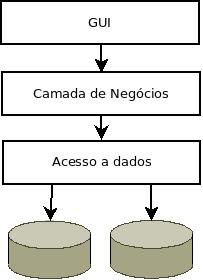
\includegraphics[width=100pt]{figuras/threelayers.jpeg}
%	\caption{Arquitetura de software da interface gráfica}
%	\label{7}
%\end{figure*}
%
%%\appendix
%
%%\chapter{ROS}












\appendix






%-------------------------------------------------------------------%


\chapter{Modelos}
\label{newmodel}

Os arquivos associados aos modelos de VANTs, utilizados no ambiente de simulação ProVANT, estão localizados na pasta referênte ao caminho:

\begin{bashcode}
$HOME/catkin\_ws/src/provant\_simulator/source/Database/simulation_elements/models/real
\end{bashcode}


Cada modelo no ambiente de simulação ProVant possui um diretório com o seu respectivo nome. Nesse diretório estão arquivos que descrevem os modelos dinâmicos, visuais, de colisão, sensoriais e da lei de controle utilizada. Portanto, caso seja necessário adicionar um novo modelo, ou editar um existente, o mesmo deve possuir(ou possui) arquivos de configuração/descrição do VANT organizados conforme os diretórios ilustrados na Figura \ref{modeloorg}., onde\\

\begin{enumerate}
\item O arquivo config.xml armazena  as informações referentes ao controlador a ser utilizado no modelo. 
\item O arquivo model.sdf descreve o modelo dinâmico, de colisão e visual do VANT para o simulador Gazebo.
\item O arquivo model.config descreve metadados do modelo.
\item O arquivo imagem.gif contém a imagem utilizada pela interface gráfica para ilustrar o modelo do VANT (vide Figura \ref{tela_inicial.jpg}, item 2).
\item O diretório meshes armazena os arquivos exportados da ferramenta CAD (utilizada para o desenvolvimento mecânico do VANT), exemplo: SolidWorks.
\end{enumerate}

\begin{figure}[H]
	\centering
	\begin{tikzpicture}[%
	grow via three points={one child at (0.5,-0.7) and
		two children at (0.5,-0.7) and (0.5,-1.4)},
	edge from parent path={(\tikzparentnode.south) |- (\tikzchildnode.west)}]
	\node {nome\_do\_modelo}
	child { node {config}
		child { node {config.xml}}
	}
	child [missing] {}
	child { node {meshes}}		
	child { node {robot}
		child { node {model.sdf}}
	}
	child [missing] {}
	child { node {model.config}}
	child { node {imagem.gif}};
	\end{tikzpicture}
	\caption{Organização do diretório com arquivos de descrição do modelo VANT}
	
	\label{modeloorg}
\end{figure}



No arquivo ''model.config'' o gazebo identifica onde está o arquivo com os dados estruturais do modelo, além de informações associadas à autoria, versão e descrição do modelo. O Código A.1 ilustra um exemplo desse arquivo. 


	\begin{minted}{xml}
	<?xml version="1.0"?>
	<model>
		<name>vant</name>
		<version>1.0</version>
		<sdf version='1.5'>robot/model.sdf</sdf>
		<author>
			<name>provant</name>
			<email>provant@ufmg.br</email>
		</author>
		<description>
			The UAV version 3.0 of the provant project 
		</description>
	</model>
	\end{minted}
	
	\centerline{Código A.1: Exemplo de conteúdo existente no arquivo ''model.config''.}
	
	\vspace{1cm}


As \textit{tags} utilizadas no arquivo ''model.config'' são:

\small
\begin{itemize}
\setlength{\itemsep}{1pt}
\setlength{\parskip}{0pt}
\setlength{\parsep}{0pt}
\item[-] \textcolor{blue}{<name></name>}: especifica o nome do modelo;
\item[-] \textcolor{blue}{<version></version>}: especifica a versão;
\item[-] \textcolor{blue}{<sdf></sdf>}: especifica o arquivo com a descrição do modelo dinâmico, de colisão e visual de modelo para o simulador Gazebo;
\item[-] \textcolor{blue}{<author><name></name></author>}\textcolor{blue}: especifica o nome do autor do modelo;
\item[-] \textcolor{blue}{<author><email></email></author>}: especifica o email para contato com o autor;
\item[-] \textcolor{blue}{<description></description>}: descreve brevemente o modelo.
\end{itemize}\normalsize


O arquivo ''config.xml'' armazena todas as configurações relativas à estrutura de controle que será utilizada durante a simulação, como: sensores, atuadores, lei de controle e período de amostragem. Com o intuíto de ajudar o usuário com a edição desse arquivo, a interface gráfica fornece ferramentas para esse propósito, não sendo necessário que o usuário acesse diretamente o arquivo. O Código A.2: ilustra um exemplo desse arquivo. 


	\begin{minted}{xml}
	<?xml version="1.0" encoding="UTF-8"?>
	<config>
		<TopicoStep>Step</TopicoStep>
		<Sampletime>12</Sampletime>
		<Strategy>libvant3_lqr.so</Strategy>
		<RefPath>ref.txt</RefPath>
		<Outputfile>out.txt</Outputfile>
		<InputPath>in.txt</InputPath>
		<ErroPath>erro.txt</ErroPath>
		<Sensors>
			<Device>Estados</Device>
		</Sensors>
		<Actuators>
			<Device>ThrustR</Device>
			<Device>ThrustL</Device>
			<Device>TauR</Device>
			<Device>TauL</Device>
			<Device>Elevdef</Device>
			<Device>Ruddef</Device>
		</Actuators>
	</config>
	\end{minted}
	
	\centerline{Código A.2: Exemplo de arquivo ''config.xml''.}
	
	\vspace{1cm}
	
	As \textit{tags} utilizadas no arquivo ''config.xml'' são:
	\small
	\begin{itemize}
	\setlength{\itemsep}{1pt}
	\setlength{\parskip}{0pt}
	\setlength{\parsep}{0pt}
	\item[-] \textcolor{blue}{<TopicoStep></TopicoStep>}: declara tópico de sincronização do simulador ao controlador. \textbf{O valor desta tag não deve ser alterado}.;
	\item[-] \textcolor{blue}{<Sampletime></Sampletime>}: define o período de amostragem do controlador, em milissegundos;
	\item[-] \textcolor{blue}{<Strategy></Strategy>}: nome da biblioteca dinâmica associada à implementação da estratégia de controle a ser utilizada em conjunto com esse modelo;
	\item[-] \textcolor{blue}{<RefPath></RefPath>}: nome do arquivo no qual os dados do sinal de referência são armazenados;
	\item[-] \textcolor{blue}{<Outputfile></Outputfile>} nome do arquivo no qual os dados dos sinais de controle são armazenados;
	\item[-] \textcolor{blue}{<InputPath></InputPath>}: nome do arquivo no qual os dados dos sensores são armazenados;
	\item[-] \textcolor{blue}{<ErroPath></ErroPath>} nome do arquivo no qual os dados do vetor de erro são armazenados;
	\item[-] \textcolor{blue}{<Sensors></Sensors>} nome dos tópicos dos sensores aos quais a estratégia de controle terá acesso (na ordem especificada)
	\item[-] \textcolor{blue}{<Actuators></Actuators>} nome dos tópicos dos atuadores aos quais a estratégia de controle terá acesso. (o controlador deve retornar um vetor com a mesma quantidade de dados e na ordem aqui especificados)
	\end{itemize}\normalsize
	\label{config.xml}

O arquivo ''model.sdf'' fornece ao Gazebo as informações do modelo do VANT no formato XML conforme o padrão SDF \footnote{\url{http://sdformat.org/spec}}. A próxima seção descreve com mais detalhes a estrutura básica de um arquivo SDF.

\section{O arquivo SDF}

Antes de apresentar a configuração básica de um arquivo SDF, é necessário primeiro introduzir algums conceitos: No simulador um modelo corresponde a um sistema mecânico, que pode ser formado por um ou múltiplos corpos rígidos\footnote{Ao assumir um corpo como rígido são desprezando efeitos de elasticidade e deformações}. Assim, como em um manipulador, no simulador os corpos são denominados elos, sendo os elos filhos conectados a elos pai através de juntas. Elos filhos são corpos rígidos que possuem movimento restringido pela conexão ("junta") com corpos denominados elos pai. Os elos possuem propriedades inerciais, visuais e de colisão. Já as juntas, impõem a restrição do movimento relativo entre dois elos, com propriedades como o tipo de junta (Prismática, rotativa, etc.), limites de movimento (Posição e velocidade), existência de atrito, etc. O Código A.3 ilustra um exemplo de arquivo SDF.
 
	\begin{minted}{xml}
	<?xml version="1.0" encoding="UTF-8"?>
	<sdf version="1.4">
		<model name="modelo">
			<link name="corpo">
				...
			</link>
			<link name="servo">
				...
			</link>
			<joint name="corpo_servo">
				...
			</joint>
		</model>
	</sdf>
	\end{minted}
	
	\centerline{Código A.3: Descrição de um elo no arquivo ''modelo.sdf''}
	
	\vspace{1cm}
	 
	 As \textit{tags} utilizadas são:
	 \small
	 \begin{itemize}
	 \setlength{\itemsep}{1pt}
	 \setlength{\parskip}{0pt}
	 \setlength{\parsep}{0pt}
	 \item[-] \textcolor{blue}{<link></link>}: especifica a existência de um elo, com o seu nome;
	 \item[-] \textcolor{blue}{<joint></joint>}: especifica a existência de uma junta, com o seu nome.  
	 \end{itemize}\normalsize
	 

Cada elo do modelo possui três tipos de descrições para o simulador: cinemática, visual e de colisão.  A estrutura de configuração de um elo em um arquivo SDF possui o formato ilustrado no Código A.4, onde:
\small
\begin{itemize}
\setlength{\itemsep}{1pt}
\setlength{\parskip}{0pt}
\setlength{\parsep}{0pt}
\item[-] \textcolor{blue}{<pose></pose>}: define a pose do elo;
\item[-] \textcolor{blue}{<inertial></inertial>}: especifica as propriedades inerciais do elo;
\item[-] \textcolor{blue}{<collision></collision>}: especifica o modelo de colisão do elo. Os modelos de colisão dos VANTs usados no ambiente de simulação são obtidos de arquivos CAD;
\item[-] \textcolor{blue}{<visual></visual>}: especifica características visuais, como cor e formato. Os modelos visuais dos VANTs usados no ambiente de simulação são obtidos de arquivos CAD, exceto a cor, que é especificada separadamente.
\end{itemize}\normalsize

	\begin{minted}{xml}
	<link name="servodir">
		<pose>0.02E-3 -277.61E-3 56.21E-3 -0.0872665 0 0</pose>
		<inertial> 
			...
		</inertial>
		<collision name="servodircollision"> <!--opcional-->
			...
		</collision>
		<visual name="servodirvisual"> <!--opcional-->
			...
		</visual>
	</link>
	\end{minted}
	\centerline{Código A.4: Descrição da de um elo no ''modelo.sdf''} 
	
	\vspace{1cm}
	


\noindent \textbf{Parâmetros de inércia do elo}: O usuário deve informar os parâmetros de inércia de cada elo na \textit{tag} ''inertial''. As informações obrigatórias são a massa, posição relativa do centro de massa e o tensor de inércia. No Código A.5 é ilustrado um exemplo de configuração dos parâmetros de inércia de um elo em formato SDF, onde:
\small
\begin{itemize}
\setlength{\itemsep}{1pt}
\setlength{\parskip}{0pt}
\setlength{\parsep}{0pt}
\item[-] \textcolor{blue}{<mass></mass>}: define a massa do elo;
\item[-] \textcolor{blue}{<pose></pose>}: especifica a posição do centro de massa do elo em relação a seu sistema de coordenadas principal;
\item[-] \textcolor{blue}{<inertia></inertia>}: especifica o tensor de inércia do elo;
\end{itemize}\normalsize


	\begin{minted}{xml}
	<inertial>
		<mass>0.0809439719362664</mass>
		<pose>
			-3.60859273452335E-10 -0.000226380714807978 0.0594780519701684 0 0 0
		</pose>
		<inertia>
			<ixx>3.88267747087835E-06</ixx>
			<ixy>6.03219085082653E-06</ixy>
			<ixz>-2.78471406661236E-12</ixz>
			<iyy>0.000104858690365283</iyy>
			<iyz>7.0486590219062E-07</iyz>
			<izz>8.31755564684115E-05</izz>		
		</inertia>
	</inertial>
	\end{minted}
	\centerline{Código A.5: Descrição de características inerciais no arquivo ''modelo.sdf''}
	
	\vspace{1cm}

\noindent \textbf{Propriedades de colisão do elo}: Para que efeitos de colisão sejam aplicados ao elo, o usuário deve descrever o formato do elo no arquivo ''model.sdf''. Existem diversas formas de descrição, porém este manual apresenta apenas o método utilizado nos modelos de VANTs do ambiente de simulação ProVANT, que consiste na importação de arquivos criados através de ferramentas CAD, como o SolidWorks. No Código A.6 mostra um exemplo de descrição dos parâmetros visuais de um elo a partir de um arquivo STL, onde:
\small
\begin{itemize}
\setlength{\itemsep}{1pt}
\setlength{\parskip}{0pt}
\setlength{\parsep}{0pt}
\item[-] \textcolor{blue}{<pose></pose>}: especifica a pose do modelo colisão em relação ao centro de coordenadas do elo;
\item[-] \textcolor{blue}{<uri></uri>}: caminho do arquivo mesh, a partir do diretório do modelo, obtido via exportação no SolidWorks; 
\end{itemize} \normalsize


	\begin{minted}{xml}
	<collision name="servodircollision">
		<pose>0 0 0 0 0 0</pose>
		<geometry>
			<mesh>
				<uri>model://vant_2comcarga/meshes/servodir.STL</uri>
			</mesh>
		</geometry>
	</collision>
	\end{minted}
	\centerline{Código A.6: Descrição de características de colisão no arquivo ''model.sdf''}

	\vspace{1cm}

\noindent \textbf{Propriedades visuais do elo}: Para que o elo seja visualizado durante a simulação, o usuário deve descrever os parâmetros visuais do elo no arquivo ''model.sdf''. Assim como no caso anterior, existem diversas formas de descrição, porém este manual ilustra apenas o método utilizado nos modelos de VANTs do ambiente de simulação, que consiste na importação de arquivos criados através de ferramentas CAD. O Código A.7 mostra um exemplo de descrição dos parâmetros visuais de um elo a partir de um arquivo STL, 	
onde: \small
\begin{itemize}
\setlength{\itemsep}{1pt}
\setlength{\parskip}{0pt}
\setlength{\parsep}{0pt}
\item[-] \textcolor{blue}{<pose></pose>}: especifica a pose que o modelo visual do elo será definido em relação ao sistema de coordenadas do elo;
\item[-] \textcolor{blue}{<uri></uri>}: caminho do arquivo mesh, a partir do diretório do modelo, obtido via exportação no SolidWorks;
\item[-] \textcolor{blue}{<ambient></ambient>}: definição de cor ambiente;
\item[-] \textcolor{blue}{<diffuse></diffuse>}: definição de cor difusa;
\item[-] \textcolor{blue}{<specular></specular>}: definição de cor especular;
\item[-] \textcolor{blue}{<emissive></emissive>}: definição de cor emissiva.
\end{itemize} \normalsize


	\begin{minted}{xml}
	<visual name="servodirvisual">
		<pose>0 0 0 0 0 0</pose>
		<geometry>
			<mesh>
				<uri>model://vant_2comcarga/meshes/servodir.STL</uri>
			</mesh>
		</geometry>
		<material>
			<ambient>0 0 0 0</ambient>
			<diffuse>1 1 1 1</diffuse>
			<specular>0.1 0.1 0.1 1</specular>
			<emissive>0 0 0 0</emissive>
		</material>
	</visual>
	\end{minted}
	\centerline{Código A.7: Descrição de características visuais no arquivo ''model.sdf''}
	

\subsection{Descrição de junta} 

Há 7 tipos de juntas no simulador: 

\begin{itemize}
	\item \textbf{revolute}: junta rotativa; 
	\item \textbf{gearbox}: junta rotativa com presença de engrenagens para transmissão de movimento angular entre elos com diferentes relações de torque e velocidade; 
	\item \textbf{revolute2}: junta composta por duas juntas rotativas em série; 
	\item \textbf{prismatic}: junta prismática; \item \textbf{universal}, junta com comportamento de uma esfera articulada; 
	\item \textbf{piston}: junta com comportamento da combinação de uma junta rotativa e uma junta prismática.
\end{itemize}

Um exemplo de estrutura de configuração de uma junta é mostrado no Código A.8, onde:
\begin{itemize}
\setlength{\itemsep}{1pt}
\setlength{\parskip}{0pt}
\setlength{\parsep}{0pt}
\item[-] \textcolor{blue}{<pose></pose>}: descreve a pose relativa em que o elo filho está em relação ao elo pai.
\item[-] \textcolor{blue}{<parent></parent>}: nome do elo pai.
\item[-] \textcolor{blue}{<child></child>}: nome do elo filho.
\item[-] \textcolor{blue}{<axis></axis>}: vetor unitário que corresponde ao eixo de rotação da junta. (expressado no sistema de coordenadas do modelo, se estiver utilizando a versão 1.4 do formato SDF; e expressado no sistema de coordenadas do elo filho, se estiver utilizando a versão 1.6 do formato SDF).
\item[-] \textcolor{blue}{<lower></lower>}: limite inferior de posição da junta (em rad, caso seja do tipo rotativa, e metros, caso seja prismática).
\item[-] \textcolor{blue}{<upper></upper>}: limite superior de posição da junta (em rad, caso seja do tipo rotativa, e metros, caso seja prismática).
\item[-] \textcolor{blue}{<velocity></velocity>}: limite de velocidade da junta (em rad/s, caso seja do tipo rotativa, e m/s, caso seja prismática).
\item[-] \textcolor{blue}{<effort></effort>}: limite de esforço da junta (em N.m, caso seja do tipo rotativa, e N, caso seja prismática).
\item[-] \textcolor{blue}{<damping></damping>}: coeficiente de atrito viscoso.
\item[-] \textcolor{blue}{<friction></friction>}: coeficiente de atrito estático.
\end{itemize}


	\begin{minted}{xml}
	<joint name="aR" type="revolute">
		<pose>0 0 0 0 0 0</pose>
		<parent>corpo</parent>
		<child>servodir</child>
		<axis>
			<xyz>0 0.9962 -0.0872</xyz>
			<limit>
				<lower>-1.5</lower>
				<upper>1.5</upper>
				<effort>2</effort>
				<velocity>0.5</velocity>
			</limit>
			<dynamics>
				<damping>0</damping>
				<friction>0</friction>
			</dynamics>
		</axis>
	</joint>
	\end{minted}
	\centerline{Código A.8: Descrição de juntas no arquivo ''model.sdf''}
	
\subsection{Descrição de plugins}
\label{plugins}

Plugins são bibliotecas dinâmicas carregadas durante a inicialização do simulador, a partir das configurações armazenadas no arquivo de descrição de modelo (arquivo SDF). Tais bibliotecas são utilizadas para a implementação de sensores e atuadores no ambiente de simulação. \\

O ambiente de simulação ProVANT utiliza apenas dois tipos de plugins existentes no simulador Gazebo para controle e monitoramento do modelo do VANT: Modelo e Sensor. Mais detalhes sobre os plugins disponibilizados no simulador Gazebo podem ser encontrados em: \url{http://gazebosim.org/tutorials/?tut=plugins\_hello\_world}

\noindent \textbf{Plugins modelo}: Plugins modelo são bibliotecas dinâmicas que controlam e monitoram variáveis de simulação do modelo VANT. Através delas, é possível criar sensores e atuadores customizados. Para inserir um plugin modelo no arquivo ''model.sdf'', o usuário deve adicionar tags <plugin></plugin>, definindo nome, nome da biblioteca dinâmica e as tags internas necessárias para configuração do plugin. O Código A.9 exemplifica o processo de inserção. 

Opções de plugins modelo disponíveis no ambiente de simulação ProVANT estão detalhados no apêndice \ref{pluginsAp}.


	\begin{minted}{xml}
	<?xml version="1.0" encoding="UTF-8"?>
	<sdf version="1.4">
		<model name="modelo">
			<link name="corpo">
				...
			</link>
			<link name="servo">
				...
			</link>
			<joint name="corpo_servo">
				...
			</joint>
			<plugin name="plugin_servo">
				...
			</plugin>
		</model>
	</sdf>
	\end{minted}
	\centerline{Código A.9: Inserção de plugins modelo no arquivo ''model.sdf''}
	
	\vspace{1cm}
	
\noindent \textbf{Plugins sensor}: Plugins sensor são bibliotecas dinâmicas que simulam sensores, portanto, são utilizados pelo ambiente de simulação ProVANT para mensurar dados de um modelo VANT. Para inserir plugins sensor basta inserir tags <sensor></sensor>, definindo nome e as tags internas necessárias para configuração do plugin. O Código A.10 exemplifica o processo de inserção.

	
	\begin{minted}{xml}
	<link name="servodir">
		<pose>0.02E-3 -277.61E-3 56.21E-3 -0.0872665 0 0</pose>
		<inertial> 
			...
		</inertial>
		<collision name="servodircollision"><!--opcional-->
			...
		</collision>
		<visual name="servodirvisual"> <!--opcional-->
			...
		</visual>
		<sensor name="servosensor"> <!--opcional-->
			...
		</sensor>
		<sensor name="servosensor2"> <!--opcional-->
			...
		</sensor>
	</link>
	\end{minted}
	\centerline{Código A.10: Inserção de plugins sensor no arquivo ''model.sdf''}

	\vspace{1cm}

Os sensores disponíveis no ambiente de simulação ProVANT são GPS, IMU, sonar e magnetômetro (Detalhes de configurações no arquivo model.sdf podem ser encontrados em \url{http://sdformat.org/spec}). No entanto, estes sensores não possuem interface de comunicação com o ROS, pois eles transmitem seus dados via tópicos do Gazebo. Para realizar a transmissão destes dados para tópicos do ROS, é necessário adicionar, juntamente aos plugins sensores, plugins modelo. Tais plugins estão especificados no apêndice \ref{pluginsAp}.

Obs.: para funcionamento correto do sensor, o usuário deve ajustar a taxa de amostragem exatamente para o inverso do passo de simulação, por exemplo 1000 HZ.

\subsection{Padrão de mensagens de comunicação}

Como padrão, todos o plugins e sensores disponíveis no ambiente de simulação disponibilizam dados através de uma mesma estrutura de dados. Esta estrutura de dados é abstraída no ROS através de mensagens. As mensagens são estruturas de dados simples, contendo campos tipados. A mensagem padrão de plugins sensores está ilustrada abaixo. 	onde:
\begin{itemize}
\item header: fornece o instante que o dado foi obtido, o frame e o número de sequência durante a comunicação.
\item name: fornece o nome do instrumento que forneceu a mensagem.
\item values: vetor composto pelos mais variados dados providos pelos sensores.
\end{itemize} 

%\begin{figure}[H]
%	\begin{minted}{xml}
%	Header header
%	string name
%	float64[] values
%	\end{minted}	
%\end{figure}

Por outro lado o controlador recebe um outro tipo de mensagem que armazena as mensagens de todos os sensores num dado passo de simulação num mesmo local e na ordem pré-definida pelo usuário, como é descrito na seção \ref{sensoresatuadores}. Tal estrutura esta ilustrada a seguir.

\begin{figure}[H]
	\begin{minted}{xml}
	Header header
	string name
	Sensor[] values
	\end{minted}
\end{figure}

\section{Modelos dos VANTs}
Nessa seção serão detalhados todos os modelos de VANTs desenvolvidos no âmbito do projeto ProVANT e disponíveis no simulador. Cada VANT será descrito mostrando seu vetor de estados, os sistemas de coordenadas utilizados para derivar o modelo cinemático e dinâmico, e tabelas com parâmetros utilizados.  

\subsection{VANT 2.0}

O primeiro modelo implementado no simulador foi o vant 2.0. O VANT foi implementado com o objetivo de simular um VANT tilt rotor simples.

\begin{figure*}[!ht]
	\centering
	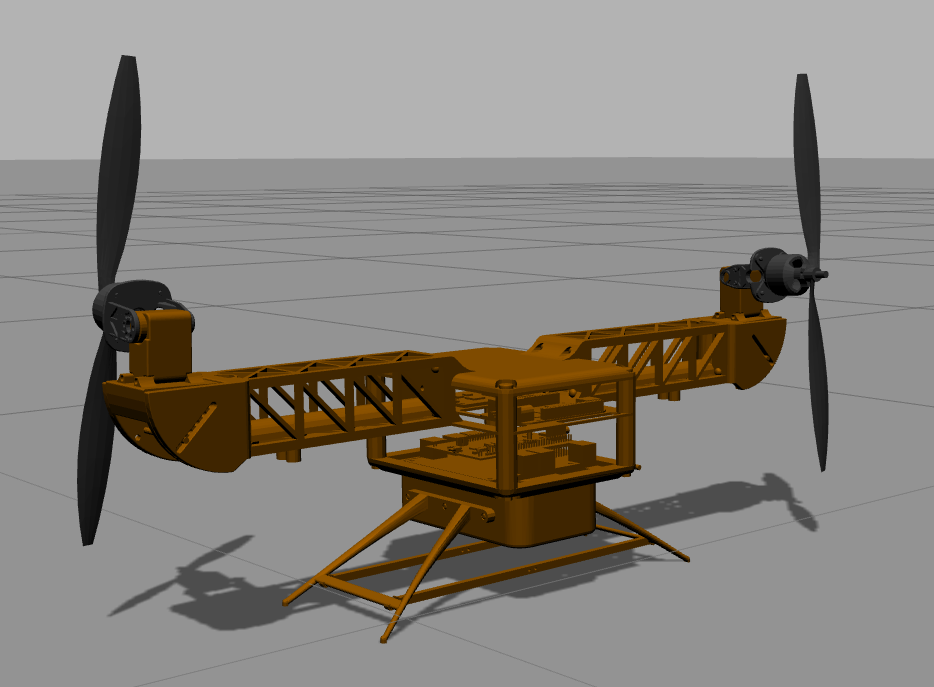
\includegraphics[width=250pt]{figuras/vant2.png}
	\caption{Modelo VANT 2.0 }
	\label{24}
\end{figure*}

O modelo cinemático e dinâmico do VANT foi desenvolvido a partir da seguinte distribuição de sistemas de coordenadas mostrados em \ref{v2frames} juntamente com os parâmetros mostrados em \ref{v2_tab}.

\begin{figure} [!ht]
	\centering
	\begin{minipage}{.5\textwidth}
		\centering
		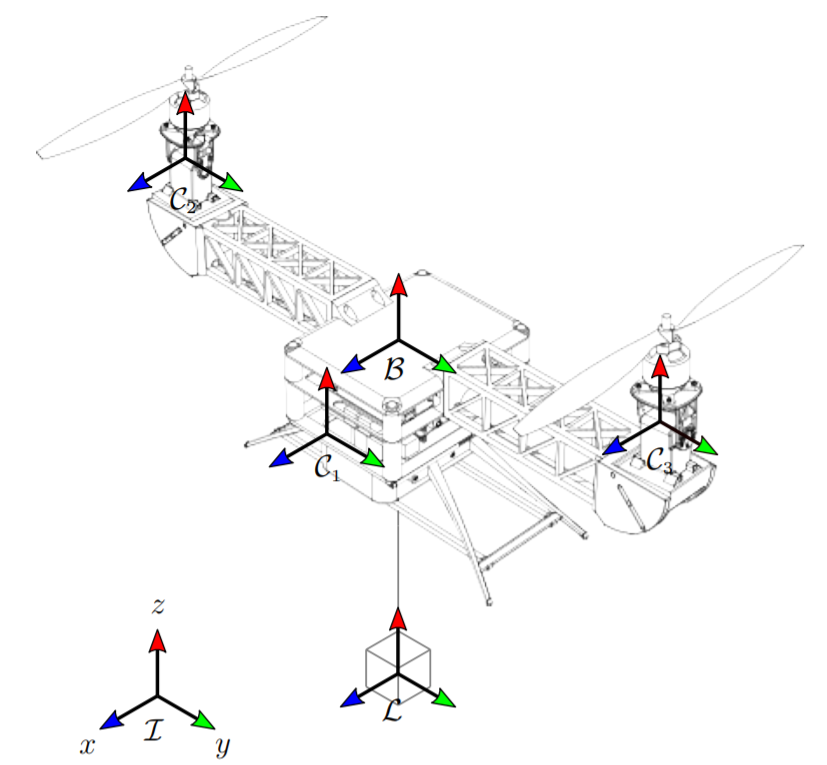
\includegraphics[width=250pt]{figuras/v2loadframes}
		\caption{Sistemas de Coordenadas do VANT 2.0.}
		\label{v2frames}
	\end{minipage}%
	\begin{minipage}{.5\textwidth}
		\centering
		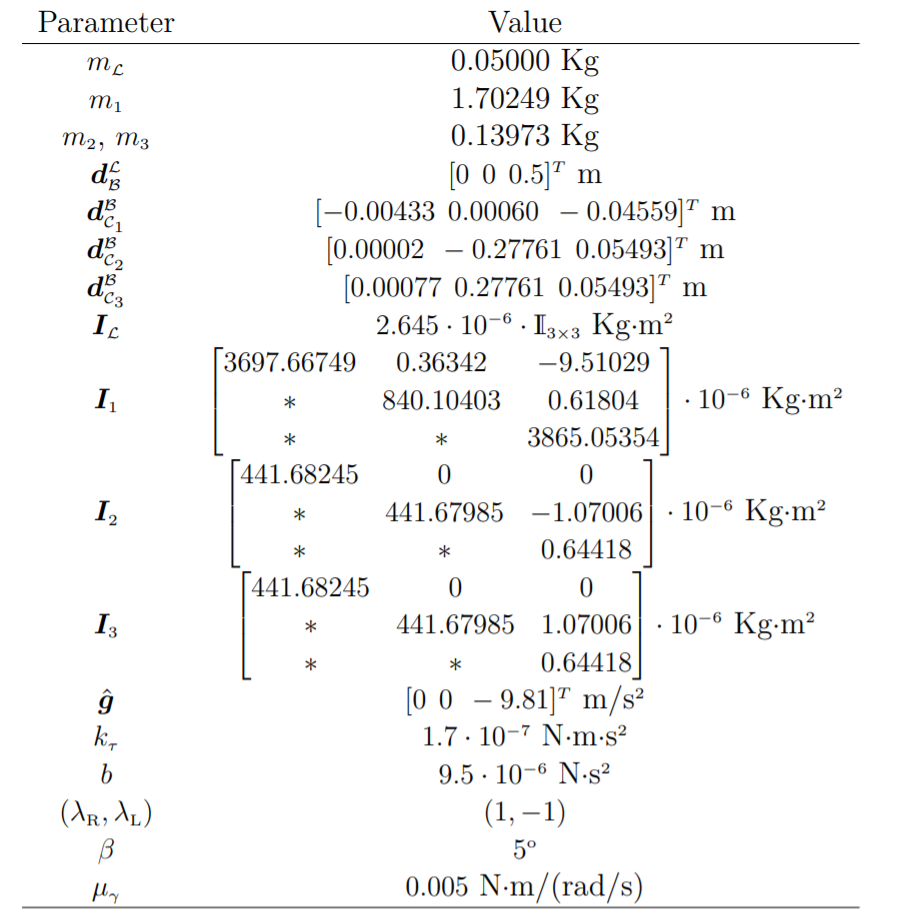
\includegraphics[width=250pt]{figuras/v2loadtab}
		\caption{Parâmetros do VANT 2.0.}
		\label{v2_tab}
	\end{minipage}
\end{figure}

O modelo foi implementado no simulador com um controlador do tipo LQR com o seguinte vetor de estados:
\begin{equation*}
\bm{X} = \begin{bmatrix}
x & y & z & \phi & \theta & \psi
\end{bmatrix}'
\end{equation*} 

Três plugins foram utilizados para a simulção do VANT 2.0 Load sendo eles: O plugin "brushless" que permite aplicar as forças geradas pelas hélices, o plugin "servo" para possibilitar atuação nos servos motores, e o plugin "statespace" para obter os estados necessarios para o controlador.Esses plugins são mais detalhados no apêndice \ref{pluginsAp}. Os tópicos, blocos retangulares, utilizados na simulação assim como os nodes, blocos circulares, presentes podem ser vistos na figura \ref{v2graph}

\begin{figure*}[!ht]
	\centering
	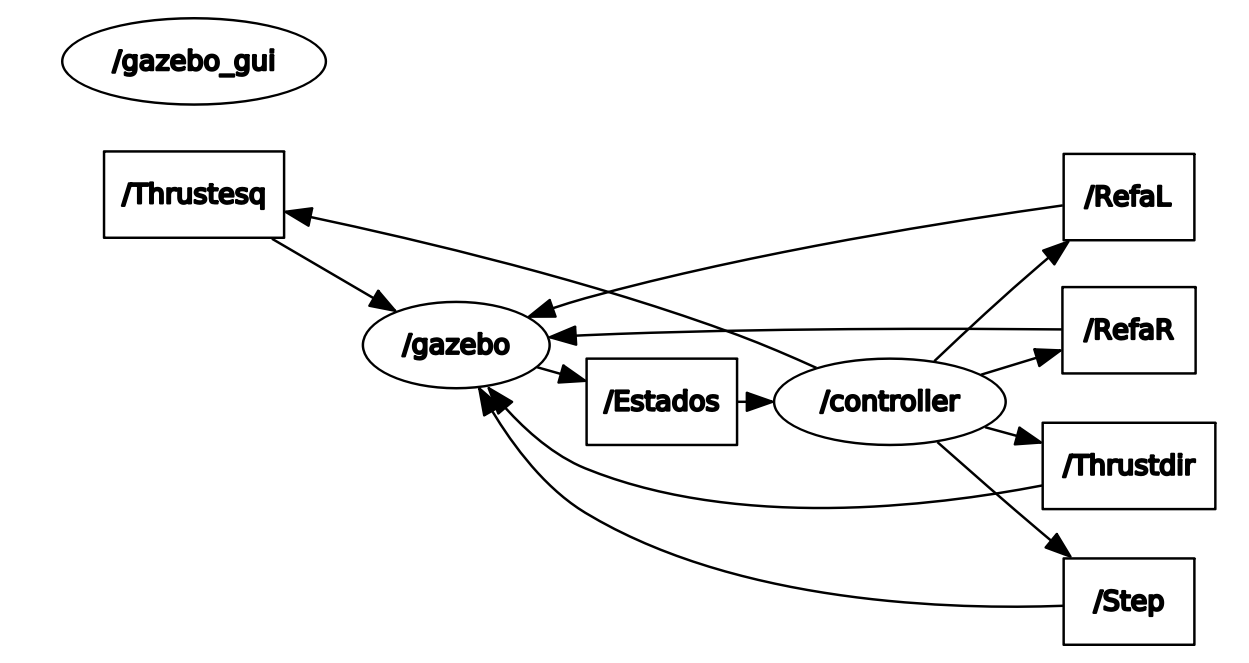
\includegraphics[width=350pt]{figuras/v2graph.png}
	\caption{Comunicação VANT 2.0}
	\label{v2graph}
\end{figure*}

\subsection{VANT 2.0 Load}


O segundo modelo implementado no simulador foi o vant 2.0 Load. O VANT foi implementado com o objetivo de simular um problema recorrente na literatura de VANTs, o problema do transporte de cargas, e foi objeto de estudos no âmbito do projeto ProVANT abordado em vários trabalhos como por exemplo nesse artigo: \url{https://www.researchgate.net/publication/327836019_Suspended_Load_Path_Tracking_Control_Using_a_Tilt-rotor_UAV_Based_on_Zonotopic_State_Estimation}.




\begin{figure*}[!ht]
	\centering
	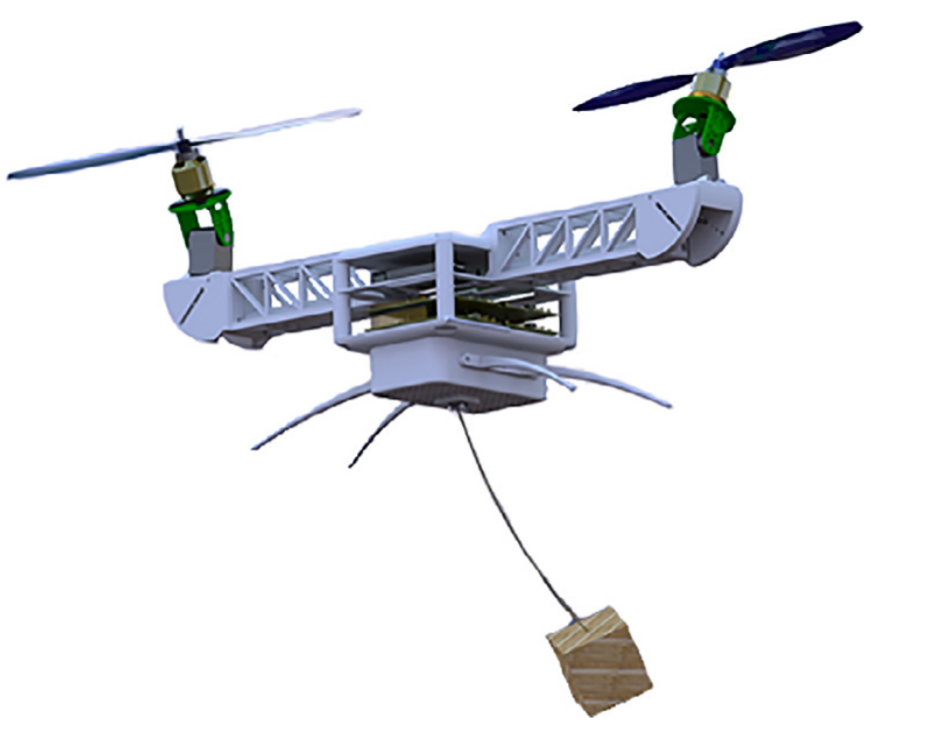
\includegraphics[width=250pt]{figuras/vant2load.png}
	\caption{VANT 2.0 Load}
	\label{25}
\end{figure*}

O modelo cinemático e dinâmico do VANT foi desenvolvido a partir da seguinte distribuição de sistemas de coordenadas juntamente com os seguinte parâmetros.

\begin{figure} [!ht]
	\centering
	\begin{minipage}{.5\textwidth}
		\centering
		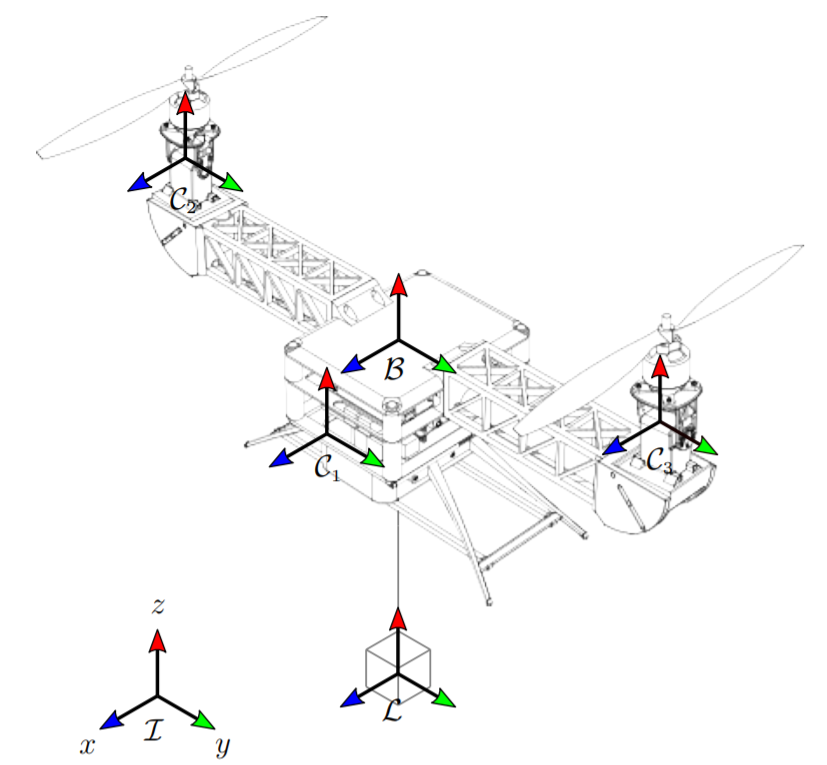
\includegraphics[width=250pt]{figuras/v2loadframes}
		\caption{Sistemas de Coordenadas do VANT 2.0 Load.}
		\label{v2loadframes}
	\end{minipage}%
	\begin{minipage}{.5\textwidth}
		\centering
		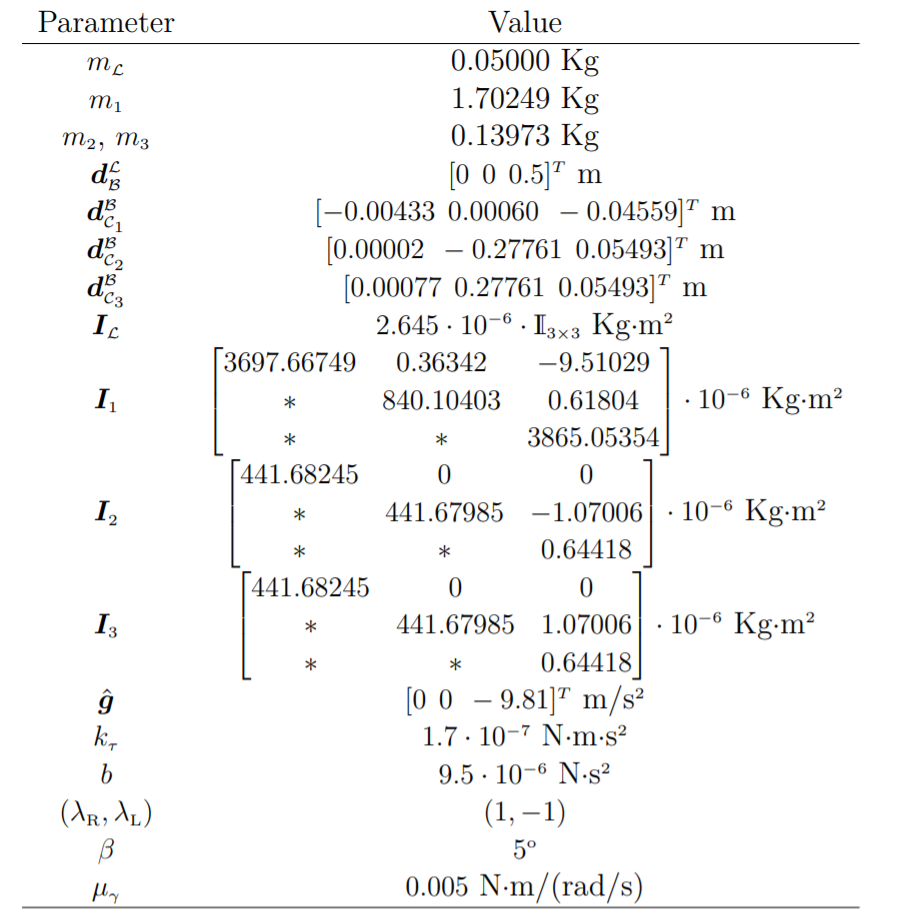
\includegraphics[width=250pt]{figuras/v2loadtab}
		\caption{Parâmetros do VANT 2.0 Load.}
		\label{v2tab}
	\end{minipage}
\end{figure}


O modelo foi implementado no simulador com um controlador do tipo $\mathcal{H}_\infty$ com o seguinte vetor de estados:
\begin{equation*}
\bm{X} = \begin{bmatrix}
\bm{q} & \bm{\dot{q}} & \int{x} & \int{y} & \int{z} & \int{\psi}
\end{bmatrix}'
\end{equation*} 

Onde, 
\begin{equation*}
\bm{q} = \begin{bmatrix}
x & y & z & \phi & \theta & \psi & x_{load} & y_{load} & \alpha_R & \alpha_L
\end{bmatrix}' 
\end{equation*} 

Três plugins foram utilizados para a simulção do VANT 2.0 Load sendo eles: O plugin "brushless" que permite aplicar as forças geradas pelas hélices, o plugin "servo" para possibilitar atuação nos servos motores, e o plugin "statespaceload" para obter os estados necessarios para o controlador.Esses plugins são mais detalhados no apêndice \ref{pluginsAp}. Os tópicos, blocos retangulares, utilizados na simulação assim como os nodes, blocos circulares, presentes podem ser vistos na figura abaixo:


\begin{figure*}[!ht]
	\centering
	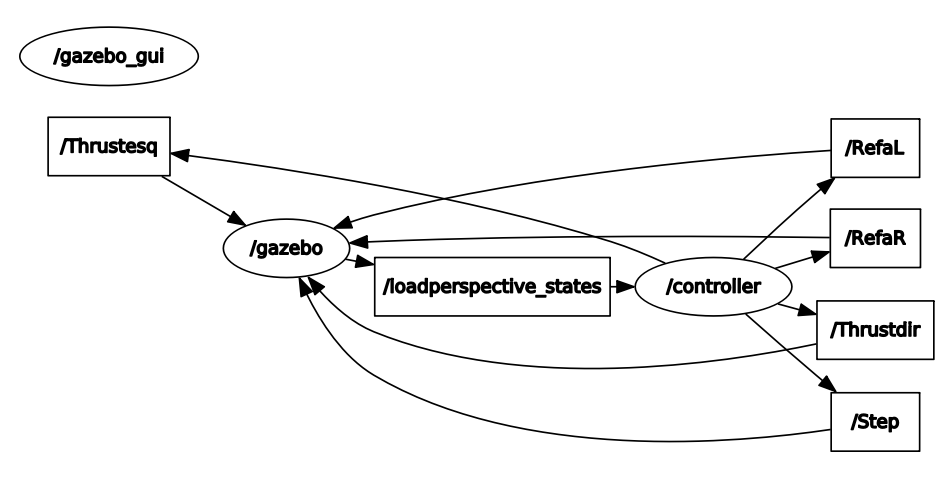
\includegraphics[width=350pt]{figuras/v2loadgraph.png}
	\caption{Comunicação VANT 2.0 Load}
	\label{v2loadgraph}
\end{figure*}


\subsection{VANT 3.0}

A partir do VANT 3.0 começou-se a utilizar superfícies aerodinâmicas de controle, uma vez que uma pequena deflexão em uma superfície aerodinâmica permite gerar forças aerodinâmicas que auxiliam no modo de voo de cruzeiro. Assim como o VANT 2.0, o VANT 3.0 foi objeto de diversos trabalhos produzidos no projeto como mostrado pelo artigo: \url{https://www.researchgate.net/publication/311919640_A_robust_adaptive_mixing_control_for_improved_forward_flight_of_a_tilt-rotor_UAV}


\begin{figure*}[!ht]
	\centering
	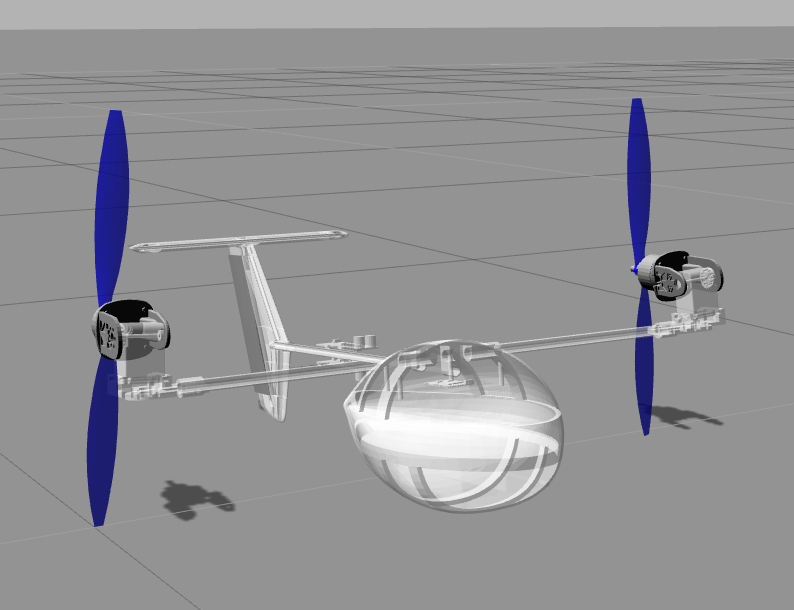
\includegraphics[width=250pt]{figuras/vant3.png}
	\caption{VANT 3.0}
	\label{27}
\end{figure*}


O modelo cinemático e dinâmico do VANT foi desenvolvido a partir da seguinte distribuição de sistemas de coordenadas juntamente com os seguinte parâmetros.

\begin{figure} [!ht]
	\centering
	\begin{minipage}{.5\textwidth}
		\centering
		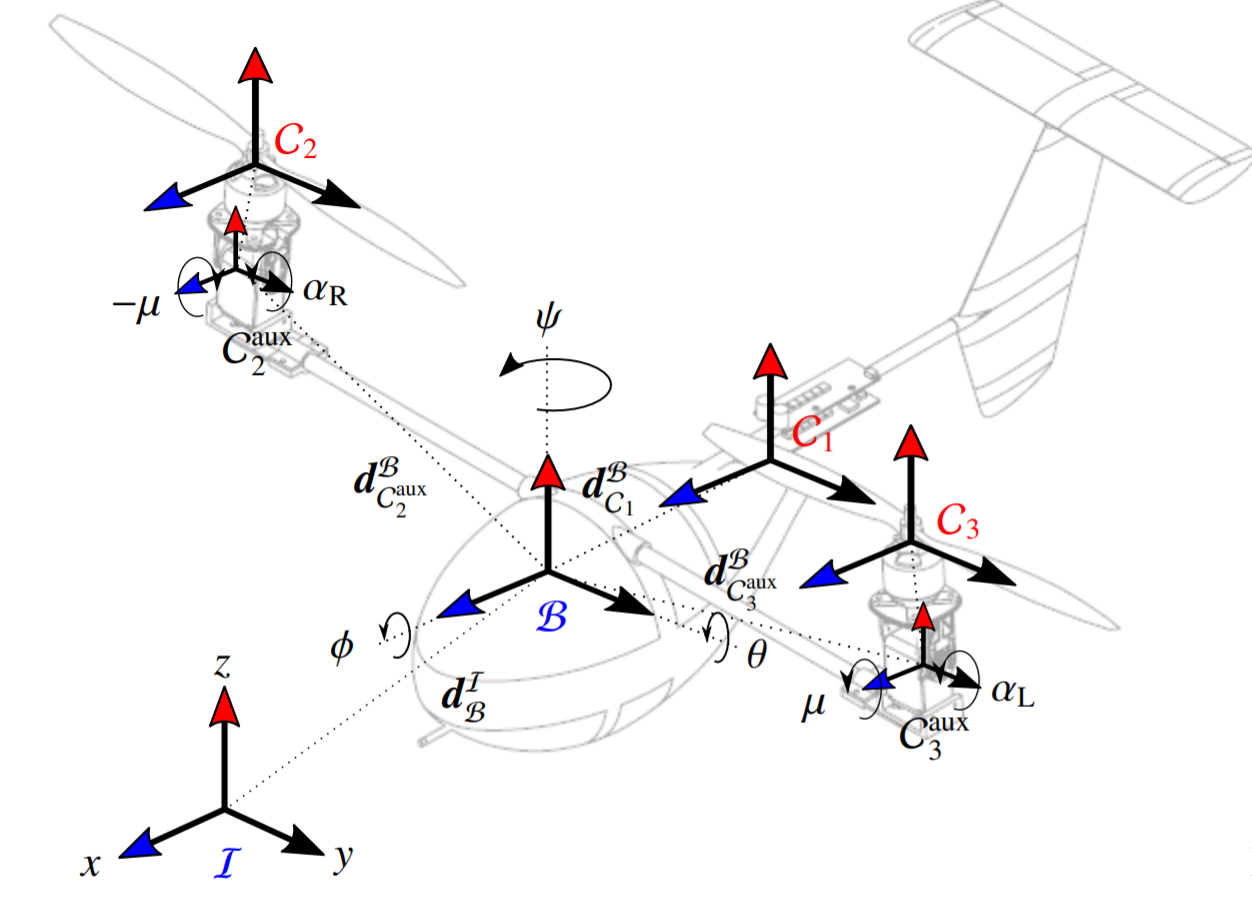
\includegraphics[width=250pt]{figuras/v3frames}
		\caption{Sistemas de Coordenadas do VANT 3.0.}
		\label{v3frames}
	\end{minipage}%
	\begin{minipage}{.5\textwidth}
		\centering
		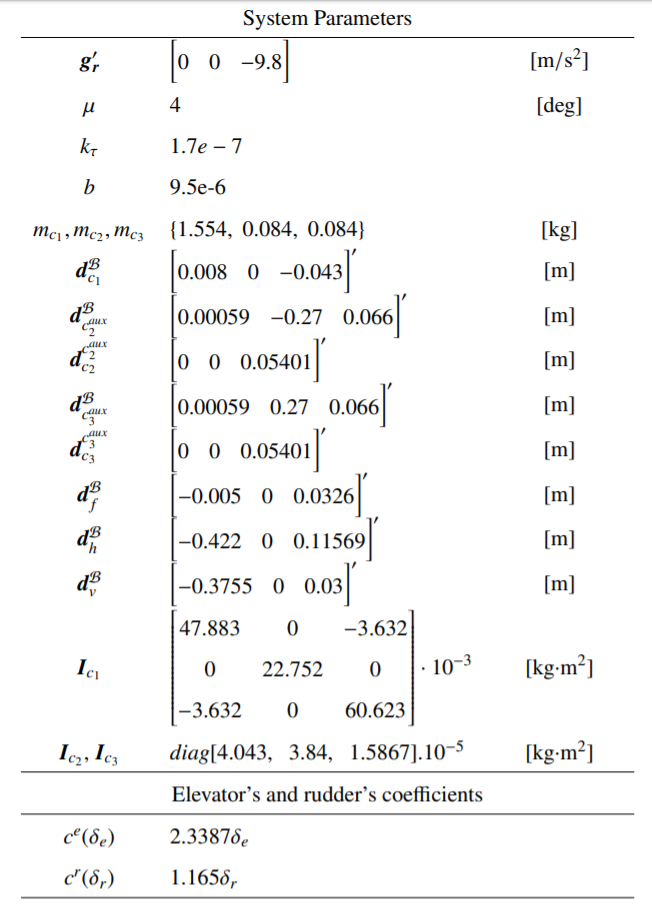
\includegraphics[width=250pt]{figuras/v3tab}
		\caption{Parâmetros do VANT 3.0.}
		\label{v3tab}
	\end{minipage}
\end{figure}

O modelo foi implementado no simulador com um controlador do tipo $\frac{\mathcal{H}_2}{\mathcal{H_\infty}}$ com o seguinte vetor de estados:
\begin{equation*}
\bm{X} = \begin{bmatrix}
u \\
 v \\
  w \\
   p \\
    q \\
     r\\
      \dot\alpha_R \\
       \dot\alpha_L \\
        z \\
         \phi \\
          \theta \\
          \psi \\
          \alpha_R \\
          \alpha_L \\
          \int{u} \\
          \int{v} \\
          \int{\psi} \\         
\end{bmatrix}
\end{equation*} 

Onde, $(u,v,w)$ são as velocidades lineares do \textit{sistema de coordenadas do corpo do VANT} em relação ao \textit{sistema de coordenadas inercial} expressado no \textit{sistema de coordenadas do corpo do VANT}, e ($p,q,r$) são as velocidades angulares do \textit{sistema de coordenadas do corpo do VANT} em relação ao \textit{sistema de coordenadas inercial} expressado no \textit{sistema de coordenadas do corpo do VANT}.

Três plugins foram utilizados para a simulção do VANT 3.0 sendo eles: O plugin "aerodinamica" que permite aplicar as forças geradas pelas hélices e controlar as superficies aerodinâmicas, o plugin "servo" para possibilitar atuação nos servos motores, e o plugin "statespace" para obter os estados necessarios para o controlador.Esses plugins são mais detalhados no apêndice \ref{pluginsAp}. Os tópicos, blocos retangulares, utilizados na simulação assim como os nodes, blocos circulares, presentes podem ser vistos na figura abaixo:


\begin{figure*}[!ht]
	\centering
	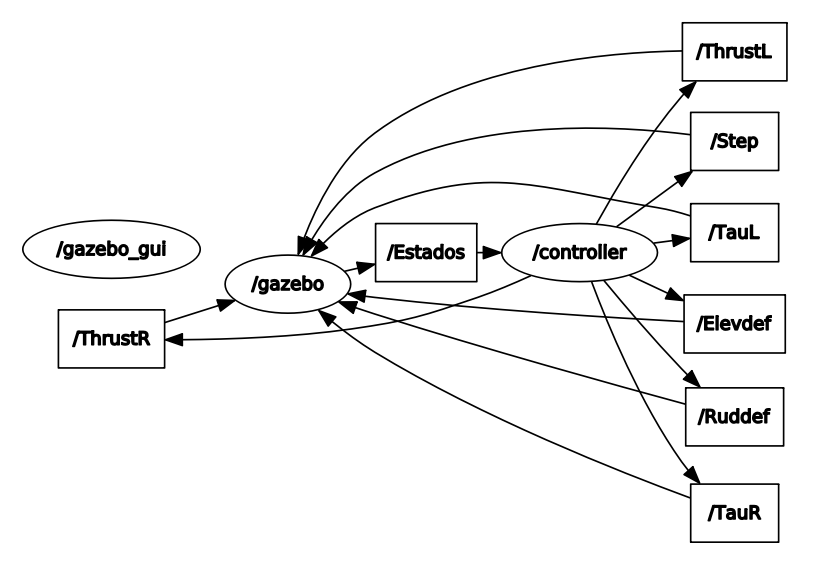
\includegraphics[width=350pt]{figuras/v3graph.png}
	\caption{Comunicação VANT 3.0}
	\label{28}
\end{figure*}


\subsection{VANT 4.0}

O VANT 4.0 foi desenvolvido em parceria com a Universidade Federal de Minas Gerais, Universidade Federal de Santa Catarina e Universidade de Sevilla com o objetivo de desenvolver um VANT de resposta rápida para situações de emergência. 

\begin{figure*}[!ht]
	\centering
	\includegraphics[width=250pt]{figuras/vant4.png}
	\caption{VANT 4.0}
	\label{29}
\end{figure*}


O modelo cinemático e dinâmico do VANT foi desenvolvido a partir da seguinte distribuição de sistemas de coordenadas juntamente com os seguinte parâmetros. Mais sobre o modelo cinemático e dinâmico do VANT ver: \url{https://www.researchgate.net/publication/337571676_Modelagem_e_Simulacao_de_um_VANT_Convertivel_Tilt-rotor}

\begin{figure} [!ht]
	\centering
	\begin{minipage}{.5\textwidth}
		\centering
		\includegraphics[width=250pt]{figuras/v4frames}
		\caption{Sistemas de Coordenadas do VANT 4.0.}
		\label{v4frames}
	\end{minipage}%
	\begin{minipage}{.5\textwidth}
		\centering
		\includegraphics[width=250pt]{figuras/v4tab}
		\caption{Parâmetros do VANT 4.0.}
		\label{v4tab}
	\end{minipage}
\end{figure}

O modelo foi implementado no simulador com um controlador do tipo $\mathcal{W}_\infty$ com o seguinte vetor de estados:
\begin{equation*}
\bm{X} = \begin{bmatrix}
\dot{\bm{q_{s}}}' & \dot{\tilde{\bm{q_{c}}}}' & \tilde{\bm{q_{c}}}' & \int_{0}^{t}{\tilde{\bm{q_{c}}}'}dt
\end{bmatrix}'
\end{equation*}

Onde, $\bm{q_{s}}$ são os graus de liberdade estabilizados, $\bm{q_{c}}$ são os graus de liberdade controlados, e $\tilde{\bm{q_{c}}} \coloneqq  \bm{q_{c}} - \bm{q_{c_{r}}}$ onde $\bm{q_{c_{r}}}$ são os valores desejados de $\bm{q_{c}}$. Além disso:
\begin{equation*}
\bm{q_{s}} = \begin{bmatrix}
\alpha_R & \alpha_L & \phi & \theta
\end{bmatrix}'
\end{equation*}
e
\begin{equation*}
\bm{q_{c}} = \begin{bmatrix}
\psi & x & y & z
\end{bmatrix}'
\end{equation*}

Para a simulação do VANT 4.0 seis plugins são utilizados: "Aerodinâmica4dot0" para implementar as forças aerodinâmicas, "statespace" para obter os estados necessários para o controlador, "servo" para atuar nos \textit{ailerons}, nos dois \textit{rudders} e nos dois rotores, "PathPlotter" para visualizar a trajetória realizada no Rviz, "VisualPropellers" para ver as hélices se movimentarem, e "DataSaveTiltRotor" para salvar dados em arquivos .txt no diretório \textit{Matlab}.Esses plugins são mais detalhados no apêndice \ref{pluginsAp}. Os tópicos, blocos retangulares, utilizados na simulação assim como os nodes, blocos circulares, presentes podem ser vistos na figura abaixo:


\begin{figure*}[!ht]
	\centering
	\includegraphics[width=350pt]{figuras/v4graph.png}
	\caption{Comunicação VANT 4.0}
	\label{30}
\end{figure*}





\subsection{Quadrotor}

O campo de estudos envolvendo VANTs do tipo quadrotor também é um campo produtivo para pesquisa, por isso foi implementado no simulador um VANT do tipo quadrotor.

\begin{figure*}[!ht]
	\centering
	\includegraphics[width=250pt]{figuras/quad.png}
	\caption{Quadrotor}
	\label{31}
\end{figure*}


O modelo cinemático e dinâmico do VANT foi desenvolvido a partir da seguinte distribuição de sistemas de coordenadas juntamente com os seguinte parâmetros.

\begin{figure} [!ht]
	\centering
	\begin{minipage}{.5\textwidth}
		\centering
		\includegraphics[width=250pt]{figuras/quadframes}
		\caption{Sistemas de Coordenadas do Qudrotor.}
		\label{quadframes}
	\end{minipage}%
	\begin{minipage}{.5\textwidth}
		\centering
		\includegraphics[width=250pt]{figuras/quad_parameters_table}
		\caption{Parâmetros do Quadrotor.}
		\label{quadtab}
	\end{minipage}
\end{figure}

O modelo foi implementado no simulador com um controlador do tipo LQR com o seguinte vetor de estados:
\begin{equation*}
\bm{X} = \begin{bmatrix}
\bm{q} & \dot{\bm{q}}
\end{bmatrix}'
\end{equation*}

Onde, 
\begin{equation*}
\bm{q} = \begin{bmatrix}
x & y & z & \phi & \theta & \psi
\end{bmatrix}'
\end{equation*}


Para a simulação do Quadrotor 4 plugins são utilizados: "QuadForces" para implementar as forçasatuando nos quatro motores, "QuadData" para obter os estados necessários para o controlador, "PathPlotter" para visualizar a trajetória realizada no Rviz, e "VisualPropellers" para ver as hélices se movimentarem.Esses plugins são mais detalhados no apêndice \ref{pluginsAp}. Os tópicos, blocos retangulares, utilizados na simulação assim como os nodes, blocos circulares, presentes podem ser vistos na figura abaixo:


\begin{figure*}[!ht]
	\centering
	\includegraphics[width=350pt]{figuras/quadgraph.png}
	\caption{Comunicação Quadrotor.}
	\label{32}
\end{figure*}


%------------------------------------------------------------------%
\chapter{Cenários}

Nesse capítulo será mostrado a organização e a estrutura a ser seguida para implementar cenários no simulador. Além disso será detalhado o processo para se adicionar novos cenários de acordo com os objetivos do usuário. Todos os cenários devem ser configurados para um VANT específico definido na configuração do cenário. No final do capítulo é apresentado um exemplo para ilustrar o procedimento apresentado.

\section{Organização}



De modo geral a estrutura de arquivos dos cenários está em duas partes. A primeira como ilustrado na Figura \ref{cenario1}. Para acessar os diretórios e arquivos abaixo deve-se seguir o seguinte caminho até o diretório "models":%, deve possuir os seguintes diretórios e arquivos: \\
\begin{bashcode}
	$HOME/catkin_ws/src/ProVANT-Simulator/source/Database/models
	\end{bashcode}
	
	\begin{figure}[H]
		\center
		\begin{tikzpicture}[%
		grow via three points={one child at (0.5,-0.7) and
			two children at (0.5,-0.7) and (0.5,-1.4)},
		edge from parent path={(\tikzparentnode.south) |- (\tikzchildnode.west)}]
		\node {Name\_of\_the\_cenario/}
		child { node {config/}
			child { node {config.xml}}
		}
		child [missing] {}
		child { node {meshes/}}		
		child { node {robot}
			child { node {model.sdf}}
		}
		child [missing] {}
		child { node {model.config}};
		\end{tikzpicture}
		\caption{Organização do diretório de cenários. Os diretórios são dados pelas estruturas retangulares com nomes terminados pelo caractere ''/'' e os arquivos possuem alguma extensão em seu nome.}
		\label{cenario1}
	\end{figure}
	
	\begin{itemize}
		\itemsep0em 
		\item[-]O arquivo ''config.xml'' armazena as informações referentes ao controlador do VANT que será utilizado na simulação do cenário.
		\item[-]O diretório ''meshes'' armazena o arquivo responsável por gerar a parte visual do cenário.
		\item[-]O arquivo ''model.sdf'' descreve o modelo visual do cenário para o simulador \textit{Gazebo}.
		\item[-]O arquivo ''model.config'' descreve metadados do modelo.
	\end{itemize}
	
	A segunda parte é onde se configura o arquivo ".world", onde é definido o VANT a ser utilizado assim como o cenário associado a ele.Para acessar os diretórios e arquivos abaixo deve-se seguir o seguinte caminho até o diretório "worlds":
	
	\begin{bashcode}
		$HOME/catkin_ws/src/ProVANT-Simulator/source/Database/worlds/worlds
		\end{bashcode}
		
		\begin{figure}[H]
			\center
			\begin{tikzpicture}[%
			grow via three points={one child at (0.5,-0.7) and
				two children at (0.5,-0.7) and (0.5,-1.4)},
			edge from parent path={(\tikzparentnode.south) |- (\tikzchildnode.west)}]
			\node {Name\_of\_the\_world/}
			child { node {Name\_of\_the\_cenario.world/}
			};
			\end{tikzpicture}
			\caption{Organização do diretório de cenários. Os diretórios são dados pelas estruturas retangulares com nomes terminados pelo caractere ''/'' e os arquivos possuem alguma extensão em seu nome.}
			\label{cenario2}
		\end{figure}
		
		\begin{itemize}
			\itemsep0em 
			\item[-]O arquivo ''.world'' é onde é definido qual VANT incluir no cenário assim como qual cenário no diretório ''models'' incluir.
		\end{itemize}
		
		
		\section{Obtendo o Cenário}
		Os cenários são obtidos a partir do download de arquivos com a extensão ".dae". A extensão DAE (Digital Asset Exchange files) é usada para transferir ativos digitais como imagens, texturas e modelos 3D entre programas gráficos.O arquivo é baseado em COLLADA, que usa um sistema baseado em XML para garantir a compatibilidade entre diferentes ferramentas gráficas. Esses arquivos podem ser obtidos em: \url{https://3dwarehouse.sketchup.com/}
		
		\begin{figure*}[!ht]
			\centering
			\includegraphics[width=450pt]{figuras/3dwh.png}
			\caption{3dwarehouse website}
			\label{33}
		\end{figure*}
		
		Uma vez escolhido o cenário desejado deve-se fazer o download como um arquivo COLLADA como mostrado na figura \ref{34} e salvar os arquivos no diretório \textit{meshes} explicitado em \ref{cenario1} 
		
		
		\begin{figure*}[!ht]
			\centering
			\includegraphics[width=350pt]{figuras/ny.png}
			\caption{Cenário}
			\label{34}
		\end{figure*}
		
		
		\begin{figure*}[!ht]
			\centering
			\includegraphics[width=150pt]{figuras/modelinfo.png}
			\caption{Numero de \textit{Polygons}}
			\label{35}
		\end{figure*}
		
		Uma vez com o arquivo do cenário faz-se necessário analisar algumas informações do modelo disponibilizadas no site 3dwarehouse. Na seção \textit{model info} da figura \ref{34} é possivel notar o parâmetro \textit{Polygon}. Uma malha poligonal é uma coleção de vértices, arestas e faces que definem a forma de um objeto 3D em computação gráfica. Uma contagem alta de \textit{Polygon} demanda muito da GPU do computador e causa uma lentidão perceptível na simulação.
		
		 Para contornar esse problema o usuário deve selecionar um cenário com uma baixa contagem de \textit{Polygon} ou utilizar de um \textit{mesh modifier} para reduzir o numero de \textit{Polygon}. Essa segunda abordagem será tratada na próxima seção.

		
		
		\section{Tratando o Cenário}
		
		Como mencionado o tratamento para reduzir o numero de \textit{Polygons} é feito utilizando de um \textit{mesh modifier}, nesse caso utilizaremos \textit{Decimate Modifier} do software de criação 3D, Blender.
		O primeiro passo é realizar a instalação do software, isso pode ser feito seguindo tutoriais disponibilizados na internet. (\textbf{COLOCAR UM TUTORIAL DA INTERNET ?????})
		Uma vez que o Blender esteja instalado deve-se importar o arquivo ".dae" do diretório \textit{meshes} e começar o processo de simplificar a malha.
		Primeiro deve-se selecionar no menu direito a opção de adicionar um modificador de malha
			\begin{figure*}[!ht]
			\centering
			\includegraphics[width=250pt]{figuras/decimod.png}
			\caption{\textit{Decimate Modifier}}
			\label{decimod}
			\end{figure*}
		
		Três opções são disponibilizadas para simplificar a malha: \textit{Collapse},\textit{Un-subdivide} e \textit{Planar}.
		\begin{itemize}
			\item \textbf{\textit{Collapse}}:
			Une os vértices progressivamente levando em consideração a forma da malha. Quatro parâmetros compõe esse modificador:
			\begin{itemize}
				\item [-] \textit{Ratio}: Define a razão de vértices colapsados. Caso seu valor seja 1 a malha não é alterada, se seu valor é 0.5 por exemplo metade das faces foram colapsadas, se seu valor for 0 todas as faces foram removidas.
				\item [-] \textit{Factor}: Define a influencia que \textit{Vertex Group}(controla qual parte da malha é modificada) tem no processo.
				\item [-] \textit{Triangulate}: Mantem as estruturas de geometria triangular.
				\item [-] \textit{Symmetry}: Mantem a simetria com relação a um eixo.
			\end{itemize}
		\begin{figure*}[!ht]
			\centering
			\includegraphics[width=200pt]{figuras/hillblendermod.png}
			\caption{\textit{\textit{Collapse}}}
			\label{collapse}
		\end{figure*}
		\item \textbf{\textit{Un-subdivide}}:Remove arestas resultantes de uma operação de \textit{subdivide}.Não é recomendado que se faça edições no arquivo depois de se usar essa opção. Um parâmetro compõe esse modificador.
		\begin{itemize}
			\item [-] \textit{Iterations}: Número de operações feitas com o modificador. Números pares são recomendados.
		\end{itemize}
	\begin{figure*}[!ht]
		\centering
		\includegraphics[width=200pt]{figuras/unsubdiv.png}
		\caption{\textit{\textit{Un-subdivide}}}
		\label{unsubdiv}
	\end{figure*}
		\item \textbf{\textit{Planar}}:Reduz detalhes de formas compostas por superfícies planas. Três parâmetros compõe esse modificador
		\begin{itemize}
			\item [-] \textit{Angle Limit}: Dissolve geometrias que apresentam ângulos maiores que o definido.
			\item [-] \textit{All Boundaries}: Geralmente utilizado quando se tem um alto valor de \textit{Angle Limit}, é usado para dissolver os vértices nos contornos das faces.
			\item [-] \textit{Delimit}: Evita dissolver geometria em alguns lugares.
		\end{itemize}
		\begin{figure*}[!ht]
		\centering
		\includegraphics[width=200pt]{figuras/planar.png}
		\caption{\textit{\textit{Planar}}}
		\label{planar}
		\end{figure*}
		\end{itemize}
		No menu esquerdo superior deve-se exportar o arquivo com a extensão definida como ".dae" para o diretório \textit{meshes} seguindo a organização mostrada em \ref{cenario1}
		
		
		\section{Configurando Cenário}
		Uma vez que o arquivo ".dae" tenha sido tratado é necessario primeiro criar um diretório com o nome do cenário no diretório "models" assim como os outros subdiretórios e arquivos necessários explicados na seção B.1.
			\begin{bashcode}
			$HOME/catkin_ws/src/ProVANT-Simulator/source/Database/models/
			\end{bashcode}
			
			
		Ao criar o arquivo "model.sdf" deve-se configura-lo como um elo visual como mostrado. Caso se deseje interação entre VANT e cenário, um modelo de colisão deve ser criado.	
			
			\begin{minted}{xml}
	<model name="nome_do_cenario">
		<pose>0 0 0  0 0 0</pose>
			<static>true</static>
				<link name="nome_do_elo">
				<visual name="nome_visual_do_cenario">
				 <pose>0 0 0 0 0 0</pose>
				  <geometry>
					<mesh>
			<uri>model://nome_do_diretório_do_cenario/meshes/nome_do_arquivo.dae</uri>
					</mesh>
				  </geometry>
				</visual>
			   </link>
			</model>
		</sdf>
		\end{minted}
		\centerline{Código B.1: Descrição do arquivo ''model.sdf'' para um cenário}	
			
		No diretório "meshes" devem ser incluídos o arquivo ".dae" modificado no Blender assim como os arquivos de textura que vêm juntamente com o arquivo ".dae".
		O arquivo "config.xml" deve ser o mesmo arquivo do VANT que se pretende usar na simulação.	
		
		\begin{minted}{xml}
	
		<config>
	    <topicdata>data</topicdata>
		<TopicoStep>Step</TopicoStep>
		<Sampletime>12</Sampletime>
		<Strategy>Estrategia_de_controle_do_VANT_desejado</Strategy>
		<RefPath>ref.txt</RefPath>
		<Outputfile>out.txt</Outputfile>
		<InputPath>in.txt</InputPath>
		<ErroPath>erro.txt</ErroPath>
		<Sensors>
			<Device>Topico_de_estados_do_VANT_desejado</Device>
		</Sensors>
		<Actuators>
			<Device>Atuador_do_VANT_desejado</Device>
			.
			.
			.
			<Device>Atuador_do_VANT_desejado</Device>
		</Actuators>
		</config>
				\end{minted}
			\centerline{Código B.2: Descrição do arquivo ''config.xml'' para um cenário}	
		
	\begin{itemize}
	\setlength{\itemsep}{1pt}
	\setlength{\parskip}{0pt}
	\setlength{\parsep}{0pt}
	\item[-] \textcolor{blue}{<Strategy></Strategy>}: especifica o binário da estratégia de controle do VANT a ser utilizado;
	\item[-] \textcolor{blue}{<Sensors></Sensors>}: tópico onde os Estados são publicados;
	\item[-] \textcolor{blue}{<Actuators></Actuators>}: tópicos que recebem as os sinais de controle do controlador e aplicam nos atuadores;
	\end{itemize} \normalsize
	
	O arquivo "model.config" deve ser configurado de forma semelhante:
	
	\begin{minted}{xml}
	<model>
		<name>nome_do_cenario</name>
		<version>1.0</version>
		<sdf version="1.4">robot/model.sdf</sdf>
		<author>
			<name></name>
			<email></email>
		</author>
		<description></description>
	</model>
	\end{minted}
	\centerline{Código B.3: Descrição do arquivo ''model.config'' para um cenário}
	
	
Por fim deve-se configurar o arquivo ".world" no diretório:
		\begin{bashcode}
	$HOME/catkin_ws/src/ProVANT-Simulator/source/Database/worlds/worlds
\end{bashcode}
	O arquivo deve ser configurado da seguinte maneira:
	
	\begin{minted}{xml}
<world name="/HOME/catkin_ws/src/ProVANT-Simulator/source/Database/worlds/worlds
/diretório_do_mundo_do_cenário/arquivo.world">
	<gravity>0 0 -9.8</gravity>
	<physics type="ode">
		<max_step_size>0.001</max_step_size>
		<real_time_factor>0</real_time_factor>
	</physics>
	<plugin name="gazebo_tutorials" filename="libgazebo_ros_world_plugin.so">
		<ok>nothil</ok>
	</plugin>
	<include>
		<uri>model://sun</uri>
		<static>true</static>
	</include>
	<include>
		<uri>model://VANT_desejado</uri>
		<name>nome_arbitrário_para_aparecer_no_Gazebo</name>
		<static>false</static>
		<pose>0 0 0 0 0 0</pose>
	</include>
	<include>
		<uri>model://cenario_desejado_do_diretório_models</uri>
		<name>nome_arbitrário_para_aparecer_no_Gazebo</name>
		<static>true</static>
		<pose>0 0 0 0 0 0</pose>
	</include>
	<scene>
		<sky>
			<time>18</time>
			<clouds>
			<speed>0</speed>
			</clouds>
		</sky>
	</scene>
</world>
</sdf>
	\end{minted}
	\centerline{Código B.4: Descrição do arquivo ''.world'' para um cenário}	
	
	\section{Exemplo}
		\subsection{VANT 4.0 Cenário}
		
	O primeiro passo é fazer o download do arquivo e utilizando a opção \textit{import} na aba \textit{File} do menu superior esquerdo do Blender abrir o arquivo ".dae" no aplicativo como mostrado na figura \ref{36}.

	\begin{figure*}[!ht]
	\centering
	\includegraphics[width=350pt]{figuras/hillblender.png}
	\caption{Cenário no software de edição 3D Blender}
	\label{36}
\end{figure*}

	No menu direito superior do aplicativo deve-se selecionar a opção \textit{modifiers} e selecionar uma das opções entre \textit{Collapse}, \textit{Un-subdivide} e \textit{Planar}. Para essa aplicação foi selecionada a opção \textit{Collapse}, para unir os vértices progressivamente, mas levando em conta a forma da malha. Nesse caso o parâmetro a ser modificado pelo usuário é o \textit{ratio}, que define a razão de vértices colapsados.Como mostrado nas seções acima um \textit{ratio} de 1 equivale a deixar a malha inalterada. É possível acompanhar o numero de faces removidas a cada utilização de um modificador na opção \textit{faces} localizada logo abaixo da opção \textit{ratio} como mostrado na figura \ref{37}. É muito importante não esquecer de clicar em \textit{Apply} após realizar as modificações para garantir que as mesmas sejam salvas.
	
	
		\begin{figure*}[!ht]
		\centering
		\includegraphics[width=250pt]{figuras/hillblendermod.png}
		\caption{\textit{Collapse} no software de edição 3D Blender}
		\label{37}
	\end{figure*}
	
	Feita as modificações desejadas deve-se, no menu superior esquerdo, ir na aba \textit{file} e selecionar a opção \textit{export} para exportar o modelo como um arquivo tipo "dae". Crie os diretórios e arquivos como mostrado na figura \ref{cenario1} e salve o arquivo no diretório \textit{meshes} do modelo do cenário. Nesse caso o arquivo se encontraria no caminho indicado por \ref{daefile} 
	
			\begin{bashcode}
	$HOME/catkin_ws/srcProVANT-Simulator/source/Database/models/cenario_hill/meshes	
		\end{bashcode}
	\label{daefile}
	
	
	
Nesse diretório também se consegue ver as texturas utilizadas pelo arquivo ".dae" como mostrado na figura \ref{38}



			\begin{figure*}[!ht]
	\centering
	\includegraphics[width=350pt]{figuras/mesheshill.png}
	\caption{Diretório \textit{meshes}}
	\label{38}
\end{figure*}


	
Deve-se então configurar o arquivo "model.sdf" do cenário. Para isso seguimos para o diretório onde esta o modelo do cenário e dentro do diretório "robot" abrir o arquivo sdf com o editor da preferência do usuário. 
				\begin{bashcode}
	$HOME/catkin_ws/src/ProVANT-Simulator/source/Database/models/cenario_hill/robot	
\end{bashcode}

			\begin{figure*}[!ht]
	\centering
	\includegraphics[width=350pt]{figuras/excenario.png}
	\caption{Exemplo "model.sdf" de um cenário}
	\label{39}
	\end{figure*}

O arquivo sdf deve conter apenas um elo com propriedades visuais como mostrado na figura \ref{39}. O arquivo "model.config" deve ser configurado de acordo então como mostrado na figura \ref{40} com a descrição apropriada.


			\begin{figure*}[!ht]
	\centering
	\includegraphics[width=350pt]{figuras/ex2cenario.png}
	\caption{Exemplo "model.config" de um cenário}
	\label{40}
\end{figure*}

Ainda no diretório do modelo do cenário deve-se por último configurar o arquivo "config.xml". Definindo o VANT a ser utilizado na simulação desse cenário como o VANT 4.0 (\ref{vant4}) faz-se necessario que tanto o arquivo "config.xml"  do VANT como do modelo do cenário sejam iguais. Isso se deve à forma em que o simulador foi desenvolvido. O arquivo configurado é mostrado na figura \ref{41}.

			\begin{figure*}[!ht]
	\centering
	\includegraphics[width=200pt]{figuras/ex3cenario.png}
	\caption{Exemplo "config.xml" de um cenário configurado para o VANT 4.0}
	\label{41}
\end{figure*}

Por fim deve-se ir ao diretório onde os arquivos ".world" são guardados e criar os diretórios e arquivos como mostrado na figura \ref{cenario2}. Nesse caso o diretório de nome Hill onde se encontra o arquivo ".world" com as configurações da simulação está no caminho \ref{worldshill} .

				\begin{bashcode}
	$HOME/catkin_ws/src/ProVANT-Simulator/source/Database/worlds/worlds/Hill	
	\end{bashcode}
\label{worldshill}

O arquivo ".world"  é configurado como mostra a figura \ref{42}


			\begin{figure*}[!ht]
	\centering
	\includegraphics[width=350pt]{figuras/ex4cenario.png}
	\caption{Exemplo ".world" de um cenário configurado para o VANT 4.0}
	\label{ex4cenario}
\end{figure*}

É importante notar as \textit{tags} que incluem o VANT e o cenário.
\begin{minted}{xml}
<include>
	<uri>model://vant_4_aerod</uri>
	<name>newmodel</name>
	<static>false</static>
	<pose>0 0 0 0 0 0</pose>
</include>
<include>
	<uri>model://cenario_hill</uri>
	<name>cenario_hill</name>
	<static>true</static>
	<pose>0 0 0 0 0 0</pose>
</include>
 \end{minted}
	\centerline{Código B.5: inclusão do VANT e modelo de cenário no arquivo ''.world'' para um cenário}


\begin{itemize}
	\itemsep0em
	\item[-] <uri></uri>: Busca o modelo no diretório \textit{models} do VANT e do cenário.
	\item[-] <name></name>: Nome do VANT e cenário que serão mostrados no gazebo
	\item[-] <static></static>: Indica se na simulação o objeto é dinâmico ou estático.
	\item[-] <pose></pose>: Para o VANT deve-se colocar a mesma \textit{pose} para qual sua simulação sem cenário foi configurada e para o cenário deve-se deixar como mostrado na imagem. 
\end{itemize}

Feito isso, a simulação está configurada e pronta para o uso. Para realizar a simulação do VANT 4.0 com o cenário apresentado basta seguir os passos do exemplo da seção 3.6.2.


			\begin{figure*}[!ht]
	\centering
	\includegraphics[width=350pt]{figuras/exhill.png}
	\caption{Simulação de um cenário configurado para o VANT 4.0}
	\label{exhill}
\end{figure*}








%----------------------------------------------------------------%


\chapter{Plugins existentes no ambiente de simulaçao ProVANT}
\label{pluginsAp}

\section{Plugins modelo}

Esta seção mostra a configuração dos plugins modelos que não tem função de transporte de dados entre Gazebo e ROS. Tais informações estão nas Tabelas \ref{tab:Brushless}, \ref{tab:QuadForces}, \ref{tab:Servo}, \ref{tab:Statespace}, \ref{tab:Statespaceload}, \ref{tab:QuadData}, \ref{tab:Aerodinamicav4},
	\ref{tab:temperature}, \ref{tab:PathPlotter},\ref{tab:VisualPropellers},  \ref{tab:UniversalJointSensor}, \ref{tab:UniversalLinkSensor} e \ref{tab:UniversalLinkSensor2}, \ref{tab:DataSaveTiltRotor}.
	% Table generated by Excel2LaTeX from sheet 'Sheet1'
	
	
	\begin{table}[h]
	\centering
	\begin{tabular}{|r|lrrr|}
	\hline
	\multicolumn{1}{|l|}{Descrição:} &  plugin para simulação das forças de empuxo resultado do giro das duas hélices  &       &       &         \\
	& pelos motores brushless de um tilt-rotor &       &       &           \\
	\hline
	\multicolumn{1}{|l|}{Arquivo:} &  libgazebo\_ros\_brushless\_plugin.so &       &       &            \\
	\hline
	\multicolumn{1}{|l|}{Configurações: } & \textcolor{blue}{<topic\_FR> </topic\_FR>}  nome do tópico refente ao valor da força a ser aplicada
	&       &       &      \\
	& na hélice direita &       &       &        \\
	&  \textcolor{blue}{<topic\_FL> </topic\_FL>}  nome do tópico refente ao valor da força a ser aplicada &       &       &        \\
	& na hélice esquerda &       &       &       \\
	& \textcolor{blue}{<LinkDir> </LinkDir>}  nome do elo correspondente à hélice direita (a força será &       &       &        \\
	& aplicada no eixo z desse elo) &       &       &        \\
	& \textcolor{blue}{<LinkEsq> </LinkEsq>}   nome do elo correspondente à hélice esquerda (a força será   &       &       &       \\
	& aplicada no eixo z desse elo) &       &       &     \\
	\hline
	\end{tabular}%
	\caption{Configuração do plugin motor brushless.}
	\label{tab:Brushless}%
	\end{table}%


%---------------------------------------------------------------------


	\begin{table}[h]
	\centering
	\begin{tabular}{|r|lrrr|}
		\hline
		\multicolumn{1}{|l|}{Descrição:} &  plugin para simulação das forças de empuxo resultado do giro das  hélices  &       &       &         \\
		& pelos motores brushless de um \textit{Quadrotor} &       &       &           \\
		\hline
		\multicolumn{1}{|l|}{Arquivo:} &  libgazebo\_ros\_QuadForces\_plugin.so &       &       &            \\
		\hline
		\multicolumn{1}{|l|}{Configurações: } & \textcolor{blue}{<topic\_F1> </topic\_F1>}  nome do tópico refente ao valor da força a ser aplicada
		&       &       &      \\
		& na hélice 1 &       &       &        \\
		&  \textcolor{blue}{<topic\_F2> </topic\_F2>}  nome do tópico refente ao valor da força a ser aplicada &       &       &        \\
		& na hélice 2 &       &       &       \\
		& \textcolor{blue}{<topic\_F3> </topic\_F3>}  nome do tópico referente ao valor da força a ser aplicada &       &       &        \\
		& na hélice 3 &       &       &        \\
		& \textcolor{blue}{<topic\_F4> </topic\_F4>}   nome do tópico referente ao valor da força a ser aplicada   &       &       &       \\
		& na hélice 4 &       &       &     \\
		& \textcolor{blue}{<body> </body>}	nome do elo onde a resultante das forças e torques será aplicada &		&
		&		\\
		& \textcolor{blue}{<DragCte> </DragCte>} Valor da constante de arrasto &		&
		&		\\
		\hline		
	\end{tabular}%
	\caption{Configuração do plugin motor brushless para um \textit{Quadrotor}.}
	\label{tab:QuadForces}%
\end{table}%

%-----------------------------------------------------------------


	
		% Table generated by Excel2LaTeX from sheet 'Sheet1'
		\begin{table}[h]
		\centering
		\begin{tabular}{|r|lr|}
		\hline
		\multicolumn{1}{|l|}{Descrição: } & plugin para simulação servo motor com funções de Torque e posição &         \\
		\hline
		\multicolumn{1}{|l|}{Arquivo: } & libgazebo\_servo\_motor\_plugin.so &          \\
		\hline
		\multicolumn{1}{|l|}{Configurações :} & \textcolor{blue}{<NameOfJoint> </NameOfJoint>} nome da junta a ser controlada pelo servo motor &          \\
		& \textcolor{blue}{<TopicSubscriber> </TopicSubscriber>} nome do tópico com valores de referência para &       \\
		& o servo motor &          \\
		& \textcolor{blue}{<LinkDir> </LinkDir>} Nome do tópico com valores de sensoriamento do servo  &        \\
		& (posição e velocidade) &      \\
		& \textcolor{blue}{<Modo> </Modo>} Modo de funcionamento do servo motor (Opções: ''Torque'' ou ''Posicao'' ) &        \\
		& \textcolor{blue}{<Force\_Saturation> </Force\_Saturation>} Valor de saturação de forças &        \\
		& \textcolor{blue}{<Angle\_Saturation> </Angle\_Saturation>} Valor de saturação do ângulo &        \\
		\hline
		\end{tabular}%
		\caption{Configuração do plugin servo-motor.}
		\label{tab:Servo}%
		\end{table}%
	
	
%-------------------------------------------------------------------	

			
		% Table generated by Excel2LaTeX from sheet 'Sheet1'
		\begin{table}[h]
		\centering
		\begin{tabular}{|r|lr|}
		\hline
		\multicolumn{1}{|l|}{Descrição: } & plugin para sensoriamento do vetor de estados de um VANT Tilt-rotor. &                \\
		& (x,y,z, $\phi$,$\theta$,$\psi$,$\alpha_R$,$\alpha_L$,$\dot{x}$,$\dot{y}$,$\dot{z}$,$\dot{\phi}$,$\dot{\theta}$,$\dot{\psi}$,$\dot{\alpha_R}$,$\dot{\alpha_L}$) 
		&             \\
		\hline
		\multicolumn{1}{|l|}{Arquivo: } & libgazebo\_AllData\_plugin.so &             \\
		\hline
		\multicolumn{1}{|l|}{Configurações: } & \textcolor{blue}{<NameOfTopic> </NameOfTopic>} nome do tópico para o usuário obter informações &        \\
		& \textcolor{blue}{<NameOfJointR> </NameOfJointR>} nome a junta do servo motor direito &            \\
		& \textcolor{blue}{<NameOfJointL> </NameOfJointL>} nome a junta do servo motor esquerdo &             \\
		& \textcolor{blue}{<bodyname> </bodyname>} nome do elo correspondente ao corpo principal do servo motor &        \\
		\hline
		\end{tabular}%
		\caption{Configuração do plugin State space.}
		\label{tab:Statespace}%
		\end{table}%	
	
	
%--------------------------------------------------------------------	
	
		
		% Table generated by Excel2LaTeX from sheet 'Sheet1'
		\begin{table}[h]
		\centering
		\begin{tabular}{|r|lr|}
		\hline
		\multicolumn{1}{|l|}{Descrição: } 
		
		& plugin para sensoriamento do vetor de estados de um VANT Tilt-rotor com a função &         \\
		& transporte de carga. &       \\
		&
		(x,y,z, $\phi$,$\theta$,$\psi$,$\alpha_R$,$\alpha_L$,$\lambda_x$,$\lambda_y$,$\dot{x}$,$\dot{y}$,$\dot{z}$,$\dot{\phi}$,$\dot{\theta}$,$\dot{\psi}$,$\dot{\alpha_R}$,$\dot{\alpha_L}$,$\dot{\lambda_x}$,$\dot{\lambda_y}$)   &  \\
		\hline
		\multicolumn{1}{|l|}{Arquivo: } & libgazebo\_AllData2\_plugin.so &          \\
		\hline
		\multicolumn{1}{|l|}{Configurações: } & \textcolor{blue}{<NameOfTopic> </NameOfTopic>} nome do tópico para o usuário obter informações &         \\
		& \textcolor{blue}{<NameOfJointR> </NameOfJointR>} nome a junta do servo motor direito &         \\
		& \textcolor{blue}{<NameOfJointL> </NameOfJointL>} nome a junta do servo motor esquerdo &        \\
		& \textcolor{blue}{<NameOfJoint\_X> </NameOfJoint\_X>} nome a junta correspondente ao grau &    \\
		& de liberdade da carga em torno do eixo X &         \\
		& \textcolor{blue}{<NameOfJoint\_Y> </NameOfJoint\_Y>} nome a junta correspondente ao grau  &        \\
		& de liberdade da carga em torno do eixo Y &         \\
		& \textcolor{blue}{<bodyname> </bodyname>} nome do elo correspondente ao corpo principal do servo &        \\
		&  motor &        \\
		\hline
		\end{tabular}%
		\caption{Configuração do plugin State space load.}
		\label{tab:Statespaceload}%
		\end{table}%		


%--------------------------------------------------------------------

	
% Table generated by Excel2LaTeX from sheet 'Sheet1'
\begin{table}[h]
	\centering
	\begin{tabular}{|r|lr|}
		\hline
		\multicolumn{1}{|l|}{Descrição: } 
		
		& plugin para sensoriamento do vetor de estados de um VANT Quadrotor  &         \\
		&
		(x,y,z, $\phi$,$\theta$,$\psi$,$\dot{x}$,$\dot{y}$,$\dot{z}$,$\dot{\phi}$,$\dot{\theta}$,$\dot{\psi}$   &  \\
		\hline
		\multicolumn{1}{|l|}{Arquivo: } & libgazebo\_QuadData\_plugin.so &          \\
		\hline
		\multicolumn{1}{|l|}{Configurações: } & \textcolor{blue}{<NameOfTopic> </NameOfTopic>} nome do tópico para o usuário obter informações &         \\
		& \textcolor{blue}{<bodyName> </bodyName>} nome do elo para obter os estados &         \\
		\hline
	\end{tabular}%
	\caption{Configuração do plugin QuadData.}
	\label{tab:QuadData}%
\end{table}%	


%-----------------------------------------------------------------



			\begin{table}[h]
	\centering			
	\begin{tabular}{|r|lr|}
		\hline
		\multicolumn{1}{|l|}{Descrição: } & plugin para aplicar as forças aerodinâmicas no VANT 4.0 &        \\
		\hline
		\multicolumn{1}{|l|}{Arquivo: } & libgazebo\_ros\_Aerodinamica4dot0.so &        \\
		\hline
		\multicolumn{1}{|l|}{Configurações:} & <topic\_AileronR>  </topic\_AileronR> nome do tópico para o usuário obter dados do aileron direito &         \\
		& \textcolor{blue}{<topic\_AileronL> </topic\_AileronL>} nome do tópico para o usuário obter dados do aileron esquerdo &        \\
		& \textcolor{blue}{<topic\_RudderR> </topic\_RudderR>} nome do tópico para o usuário obter dados do rudder direito &        \\
		& \textcolor{blue}{<topic\_RudderL> </topic\_RudderL>}  nome do tópico para o usuário obter dados do rudder esquerdo &        \\
		& \textcolor{blue}{<topic\_Fr> </topic\_Fr>} nome do tópico para o usuário obter dados das forças aplicadas  &         \\
		& pela hélice direita &         \\
		& \textcolor{blue}{<topic\_Fl> </topic\_Fl>} nome do tópico para o usuário obter dados das forças aplicadas &    	\\
		& pela hélice esquerda &		\\	
		& \textcolor{blue}{<MainBody> </MainBody>} elo referente ao corpo principal & \\
		& \textcolor{blue}{<LinkFr> </LinkFr>} elo referente ao grupo propulsor onde a força da hélice direita atua &      \\
		& \textcolor{blue}{<LinkFl> </LinkFl>} elo referente ao grupo propulsor onde a força da hélice esquerda atua &      \\
		& \textcolor{blue}{<LinkAileronR> </LinkAileronR>} elo referente ao aileron direito &     \\
		& \textcolor{blue}{<LinkAileronL> </LinkAileronL>} elo referente ao aileron esquerdo &		\\
		& \textcolor{blue}{<LinkRudderR> </LinkRudderR>} elo referente ao rudder esquerdo &		\\
		& \textcolor{blue}{<LinkRudderL> </LinkRudderL>} elo referente ao rudder esquerdo &		\\
		& \textcolor{blue}{<CentroAerod\_F> </CentroAerod\_F>} elo referente ao centro aerodinâmico da fuselagem &		\\
		& \textcolor{blue}{<CentroAerod\_Wr> </CentroAerod\_Wr>} elo referente ao centro aerodinâmico da asa direita &		\\
		& \textcolor{blue}{<CentroAerod\_Wl> </CentroAerod\_Wl>} elo referente ao centro aerodinâmico da asa esquerda &		\\
		& \textcolor{blue}{<CentroAerod\_RudR> </CentroAerod\_RudR>} elo referente ao centro aerodinâmico do rudder direito &		\\
		& \textcolor{blue}{<CentroAerod\_RudL> </CentroAerod\_RudL>} elo referente ao centro aerodinâmico do rudder esquerdo &		\\
		\hline
	\end{tabular}%
	\caption{Configuração do plugin Aerodinâmica.}
	\label{tab:Aerodinamicav4}%
\end{table}%



%----------------------------------------------------------------
		
		
				
			% Table generated by Excel2LaTeX from sheet 'Sheet1'
			\begin{table}[h]
			\centering			
			\begin{tabular}{|r|lr|}
			\hline
			\multicolumn{1}{|l|}{Descrição: } & plugin para sensoriamento da temperatura e pressão atmosférica com ruído. &        \\
			\hline
			\multicolumn{1}{|l|}{Arquivo: } & libgazebo\_ros\_temperature.so &        \\
			\hline
			\multicolumn{1}{|l|}{Configurações:} & <Topic> </Topic> nome do tópico para o usuário obter dados  &         \\
			&  sensoriais &        \\
			& \textcolor{blue}{<TempOffset> </TempOffset>} offset de erro para dados de temperatura ruidosos &        \\
			& \textcolor{blue}{<TempStandardDeviation> </TempStandardDeviation>} desvio padrão de erro para dados de &         \\
			& temperatura ruidosos &         \\
			& \textcolor{blue}{<BaroOffset> </BaroOffset>} offset de erro para dados de pressão ruidosos &        \\
			& \textcolor{blue}{<BaroStandardDeviation> </BaroStandardDeviation>} desvio padrão de erro para dados de &         \\
			& pressão ruidosos &         \\
			& \textcolor{blue}{<maxtemp> </maxtemp>} valor máximo de temperatura &    \\
			& \textcolor{blue}{<mintemp> </mintemp>} valor mínimo de temperatura & \\
			& \textcolor{blue}{<maxbaro> </maxbaro>} valor máximo de pressão &      \\
			& \textcolor{blue}{<minbaro> </minbaro>} valor mínimo de pressão &      \\
			& \textcolor{blue}{<Nbits> </Nbits>} quantidade de bits utilizados na digitalização &     \\
			\hline
			\end{tabular}%
			\caption{Configuração do plugin Temperature.}
			\label{tab:temperature}%
			\end{table}%
		
		
%---------------------------------------------------------------------



\begin{table}[h]
	\centering			
	\begin{tabular}{|r|lr|}
		\hline
		\multicolumn{1}{|l|}{Descrição: } & plugin para visualizar trajetória do VANT no Rviz. &        \\
		\hline
		\multicolumn{1}{|l|}{Arquivo: } & libgazebo\_ros\_PathPlotter.so &        \\
		\hline
		\multicolumn{1}{|l|}{Configurações:} & \textcolor{blue}{<NameOfPathTopic> </NameOfPathTopic>} nome do tópico para o usuário publicar dados  &         \\
		&  da trajetória real do VANT &        \\
		& \textcolor{blue}{<NameOfPathRefTopic> </NameOfPathRefTopic>} nome do tópico para o usuário publicar dados &        \\
		& da trajetória de referência do VANT &		\\
		& \textcolor{blue}{<NameOfMarkerTopic> </NameOfMarkerTopic>} nome do tópico para publicar as informações &         \\
		& visuais do VANT &         \\
		& \textcolor{blue}{<bodyName> </bodyName>} elo principal utilizado como referência para se obter dados necessários  &        \\
		& \textcolor{blue}{<uav> </uav>} VANT utilizado na simulação &         \\
		\hline
	\end{tabular}%
	\caption{Configuração do plugin PathPlotter.}
	\label{tab:PathPlotter}%
\end{table}%



%-----------------------------------------------------------------------


\begin{table}[h]
	\centering			
	\begin{tabular}{|r|lr|}
		\hline
		\multicolumn{1}{|l|}{Descrição: } & plugin para permitir movimentação das hélices do VANT. &        \\
		\hline
		\multicolumn{1}{|l|}{Arquivo: } & libgazebo\_ros\_VisualPropellers.so &        \\
		\hline
		\multicolumn{1}{|l|}{Configurações:} & \textcolor{blue}{<Propeller1> </Propeller1>} junta referente à hélice de número 1  &         \\
		& \textcolor{blue}{<Propeller2> </Propeller2>} junta referente à hélice de número 2 &        \\
		& \textcolor{blue}{<Propellers\_Velocity> </Propellers\_Velocity>} Valor desejado da velocidade das hélices &         \\
		\hline
	\end{tabular}%
	\caption{Configuração do plugin VisualPropellers.}
	\label{tab:VisualPropellers}%
\end{table}%


%--------------------------------------------------------------------



			% Table generated by Excel2LaTeX from sheet 'Sheet1'
			\begin{table}[h]
			\centering
			\begin{tabular}{|r|lr|}
			\hline
			\multicolumn{1}{|l|}{Descrição: } & plugin para sensoriamento de todos os dados que o Gazebo disponibiliza de uma junta. &         \\
			&  (ângulo, velocidade angular e Torque) &        \\
			\hline
			\multicolumn{1}{|l|}{Arquivo: } & libgazebo\_ros\_universaljoint.so &    \\
			\hline
			\multicolumn{1}{|l|}{Configurações:} & <NameOfTopic> </NameOfTopic> nome do tópico para o usuário obter dados sensoriais &      \\
			& \textcolor{blue}{<NameOfJoint> </NameOfJoint>} nome da junta para sensoriamento &     \\
			& \textcolor{blue}{<Axis> </Axis>} Eixo de rotação da junta (''axis'' para primeira junta  &    \\
			& e ''axis2'' para segunda junta - gazebo contém juntas q permite dois graus de liberdade) &     \\
			\hline
			\end{tabular}%
			\caption{Configuração do plugin UniversalJointSensor.}
			\label{tab:UniversalJointSensor}%
			\end{table}%

%----------------------------------------------------------------------


				% Table generated by Excel2LaTeX from sheet 'Sheet1'
				\begin{table}[h]
				\centering
				\begin{tabular}{|rr|lrr|}
				\hline
				\multicolumn{1}{|l}{Descrição: } &       & plugin para sensoriamento de todos os dados que o Gazebo disponibiliza de um elo. &       &     \\
				\hline
				\multicolumn{1}{|l}{Arquivo: } &       & libgazebo\_ros\_universallink.so &       &         \\
				\hline
				\multicolumn{1}{|l}{Configurações: } &       & \textcolor{blue}{<NameOfTopic> </NameOfTopic>} nome do tópico para o usuário obter dados sensoriais &           &  \\
				&       & \textcolor{blue}{<NameOfLink> </NameOfLink>} nome da elo para sensoriamento &        &  \\
				\hline
				\end{tabular}%
				\caption{Configuração do plugin UniversalLinkSensor.}
				\label{tab:UniversalLinkSensor}%
				\end{table}%


%------------------------------------------------------------------------



			% Table generated by Excel2LaTeX from sheet 'Sheet1'
			\begin{table}[h]
			\centering
			\begin{tabular}{|rr|lrr|}
			\hline
			\multicolumn{1}{|l}{Ordem de informações:} &       & pose relativa em x &       &  \\
			&       & pose relativa em y &       &         \\
			&       & pose relativa em z &       &         \\
			&       & pose relativa em phi &       &       \\
			&       & pose relativa em theta &       &       \\
			&       & pose relativa em   psi &       &       \\
			&       & velocidade relativa em x &       &       \\
			&       & velocidade relativa em y &       &       \\
			&       & velocidade relativa em z &       &       \\
			&       & aceleração linear relativa em x &       &        \\
			&       & aceleração linear relativa em y &       &        \\
			&       & aceleração linear relativa em z &       &        \\
			&       & força relativa em x &       &         \\
			&       & força relativa em y &       &         \\
			&       & força relativa em z &       &         \\
			&       & velocidade angular relativa em x        &       &  \\
			&       & velocidade angular relativa em y        &       &  \\
			&       & velocidade angular relativa em z        &       &  \\
			&       & aceleração angular relativa em x        &       &  \\
			&       & aceleração angular relativa em y        &       &  \\
			&       & aceleração angular relativa em z        &       &  \\
			&       & conjugado mecânico relativa em x        &       &  \\
			&       & conjugado mecânico relativa em y        &       &  \\
			&       & conjugado mecânico relativa em z        &       &  \\
			&       & pose global em x      &       &  \\
			&       & pose global em y      &       &  \\
			&       & pose global em z      &       &  \\
			&       & pose global em phi         &       &  \\
			&       & pose global em theta &       &        \\
			&       & pose global em psi  &       &        \\
			&       & velocidade global em x &       &         \\
			&       & velocidade global em y &       &         \\
			&       & velocidade global em z &       &        \\
			&       & aceleração linear global em x &       &    \\
			&       & aceleração linear global em y &       &    \\
			&       & aceleração linear global em z &       &    \\
			&       & força global em x &             &  \\
			&       & força global em y &              &  \\
			&       & força global em z &              &  \\
			&       & velocidade angular global em x     &       &  \\
			&       & velocidade angular global em y    &       &  \\
			&       & velocidade angular global em z     &       &  \\
			&       & aceleração angular global em x    &       &  \\
			&       & aceleração angular global em y    &       &  \\
			&       & aceleração angular global em z    &       &  \\
			&       & conjugado mecânico global em x    &       &  \\
			&       & conjugado mecânico global em y    &       &  \\
			&       & conjugado mecânico global em z    &       &  \\
			&       & velocidade linear do centro de gravidade global em x &           &  \\
			&       & velocidade linear do centro de gravidade global em y &           &  \\
			&       & velocidade linear do centro de gravidade global em z &           &  \\
			&       & pose linear do centro de gravidade global em x &       &       \\
			&       & pose linear do centro de gravidade global em y &       &       \\
			&       & pose linear do centro de gravidade global em z &       &       \\
			\hline
			\end{tabular}%
			\caption{Ordem de dados do plugin UniversalLinkSensor.}
			\label{tab:UniversalLinkSensor2}%
			\end{table}%
%---------------------------------------------------------------------

				\begin{table}[h]
	\centering
	\begin{tabular}{|rr|lrr|}
		\hline
		\multicolumn{1}{|l}{Descrição: } &       & plugin para salvar dados no diretório matlab. &       &     \\
		\hline
		\multicolumn{1}{|l}{Arquivo: } &       & libgazebo\_ros\_DataSaveTiltRotor.so &       &         \\
		\hline
		\multicolumn{1}{|l}{Configurações: } &       & \textcolor{blue}{<topic\_Fr> </topic\_Fr>} nome do tópico para o usuário obter dados das forças na hélice direita&           &  \\
		&       & \textcolor{blue}{<topic\_Fl> </topic\_Fl>}nome do tópico para o usuário obter dados das forças na hélice esquerda &        &  \\
		&       & \textcolor{blue}{<topic\_DAr> </topic\_DAr>}nome do tópico para o usuário obter dados da deflexão no aileron direito &        &  \\
		&       & \textcolor{blue}{<topic\_DAl> </topic\_DAl>}nome do tópico para o usuário obter dados da deflexão no aileron esquerdo &        &  \\
		&       & \textcolor{blue}{<topic\_DRr> </topic\_DRr>}nome do tópico para o usuário obter dados da deflexão no rudder direito &        &  \\
		&       & \textcolor{blue}{<topic\_DRl> </topic\_DRl>}nome do tópico para o usuário obter dados da deflexão no rudder esquerdo &        &  \\
		&       & \textcolor{blue}{<Fr\_sat> </Fr\_sat>}valor de saturação da força aplicada na hélice direita &        &  \\
		&       & \textcolor{blue}{<Fl\_satl> </Fl\_sat>}valor de saturação da força aplicada na hélice esquerda &        &  \\
		&       & \textcolor{blue}{<DAr\_satl> </DAr\_satl>}valor de saturação da deflexão no aileron direito &        &  \\
		&       & \textcolor{blue}{<DAl\_satl> </DAl\_satl>}valor de saturação da deflexão no aileron esquerdo &        &  \\
		&       & \textcolor{blue}{<DRr\_satl> </DRr\_satl>}valor de saturação da deflexão no rudder direito &        &  \\
		&       & \textcolor{blue}{<DRl\_satl> </DRl\_satl>}valor de saturação da deflexão no rudder esquerdo &        &  \\	
		\hline
	\end{tabular}%
	\caption{Configuração do plugin DataSaveTiltRotor.}
	\label{tab:DataSaveTiltRotor}%
\end{table}%

			
%----------------------------------------------------------------------				

	\section{Plugins modelo para uso junto aos plugins Sensors}

		Esta seção mostra a configuração dos plugins modelos que tem função de transporte de dados entre Gazebo e ROS. Tais informações estão nas tabelas \ref{tab:GPS},\ref{tab:IMU},\ref{tab:Sonar} e \ref{tab:magnetometro}.

		% Table generated by Excel2LaTeX from sheet 'Sheet1'
		\begin{table}[h]
		\centering
		\begin{tabular}{|r|lrrr|}
		\hline
		\multicolumn{1}{|l|}{Descrição: } & plugin para transmitir dados do sensor GPS para ROS. &       &       &     \\
		\hline
		\multicolumn{1}{|l|}{Arquivo: } & libgazebo\_ros\_gps.so &       &        &  \\
		\hline
		\multicolumn{1}{|l|}{Configurações: } & \textcolor{blue}{<gazebotopic> </gazebotopic>} nome do tópico do gazebo onde GPS publica dados &       &       &         \\
		& \textcolor{blue}{<rostopic> </rostopic>} tópico do ROS &       &       &         \\
		& \textcolor{blue}{<link> </link>} nome do  que o GPS está acoplado &       &       &   \\
		\hline
		\end{tabular}%
		\caption{Configuração do plugin modelo para transmissão de dados do GPS dos tópicos do Gazebo para tópicos do ROS.}
		\label{tab:GPS}%
		\end{table}%
		
		% Table generated by Excel2LaTeX from sheet 'Sheet1'
		\begin{table}[h]
		\centering
		\begin{tabular}{|r|lrrr|}
		\hline
		\multicolumn{1}{|l|}{Descrição: } & plugin para transmitir dados do sensor IMU para ROS &       &       &     \\
		\hline
		\multicolumn{1}{|l|}{Arquivo: } & libgazebo\_imu\_gps.so &       &        &  \\
		\hline
		\multicolumn{1}{|l|}{Configurações: } & \textcolor{blue}{<gazebotopic> </gazebotopic>} nome do tópico do gazebo onde IMU publica dados &       &       &      \\
		& \textcolor{blue}{<rostopic> </rostopic>} tópico do ROS &       &       &      \\
		& \textcolor{blue}{<link> </link>} nome do elo que o IMU está acoplado &       &       &   \\
		\hline
		\end{tabular}%
		\caption{Configuração do plugin modelo para transmissão de dados do IMU dos tópicos do Gazebo para tópicos do ROS.}
		\label{tab:IMU}%
		\end{table}%
		
			% Table generated by Excel2LaTeX from sheet 'Sheet1'
			\begin{table}[h]
			\centering
			\begin{tabular}{|r|lr|}
			\hline
			\multicolumn{1}{|l|}{Descrição: } & plugin para transmitir dados do sensor sonar para ROS. &       \\
			\hline
			\multicolumn{1}{|l|}{Arquivo: } & libgazebo\_ros\_sonar.so &            \\
			\hline
			\multicolumn{1}{|l|}{Configurações: } & \textcolor{blue}{<gazebotopic> </gazebotopic>} nome do tópico do gazebo onde sonar publica dados &           \\
			& \textcolor{blue}{<rostopic> </rostopic>} tópico do ROS &           \\
			& \textcolor{blue}{<link> </link>} nome do elo que o sonar está acoplado &     \\
			\hline
			\end{tabular}%
			\caption{Configuração do plugin modelo para transmissão de dados do Sonar dos tópicos do Gazebo para tópicos do ROS.}
			\label{tab:Sonar}%
			\end{table}%
			
			% Table generated by Excel2LaTeX from sheet 'Sheet1'
			\begin{table}[h]
			\centering
			\begin{tabular}{|r|lr|}
			\hline
			\multicolumn{1}{|l|}{Descrição: } & plugin para transmitir dados do sensor magnetômetro para ROS. &                \\
			\hline
			\multicolumn{1}{|l|}{Arquivo: } & libgazebo\_ros\_magnetometro.so &                    \\
			\hline
			\multicolumn{1}{|l|}{Configurações: } & <gazebotopic> </gazebotopic> nome do tópico do gazebo onde magnetometro publica dados &             \\
			& \textcolor{blue}{<rostopic> </rostopic>} magnetometro está acoplado &                    \\
			& \textcolor{blue}{<link> </link>} nome do elo que o magnetômetro está acoplado &                   \\
			\hline
			\end{tabular}%
			\caption{Configuração do plugin modelo para transmissão de dados do Magnetômetro dos tópicos do Gazebo para tópicos do ROS.}
			\label{tab:magnetometro}%
			\end{table}%
				
	
		


\chapter{CMakeLists.txt}
\label{cmake}

Esta seção foi extraída da página \url{http://wiki.ros.org/catkin/CMakeLists.txt} no dia 25/08/2017, visite-a para mais informações.

\section{Visão geral e estrutura do arquivo CMakeLists.txt}

O arquivo CMakeLists.txt armazena comandos de compilação e instalação de pacotes de software. Necessariamente, o arquivo \textbf{deve seguir o formato e a ordem a seguir}. 

\begin{enumerate}
	\setlength{\itemsep}{1pt}
	\setlength{\parskip}{0pt}
	\setlength{\parsep}{0pt}
	\item Versão CMake necessária (cmake\_minimum\_required)
	\item Nome do pacote (project())
	\item Encontrar outros pacotes CMake/Catkin necessários para compilação (find\_package())
	\item Habilitação de suporte para módulos Python (catkin\_python\_setup())
	\item Geradores de Mensagens/Serviços/Ações do ROS (add\_message\_files(), add\_service\_files(), add\_action\_files())
	\item Invocar geração de Mensagem/Serviço/Ação (generate\_messages())
	\item Especificar pacote  de compilação, informação e exportação (catkin\_package())
	\item Bibliotecas/Executáveis para compilação (add\_library()/add\_executable()/target\_link\_libraries())
	\item Testes de construção (catkin\_add\_gtest())
	\item Regras de instalação (install())	
\end{enumerate}

\section{Versão CMake}

Todo arquivo CMakeLists.txt deve começar com a declaração da versão do sistema. A versão requisitada é a 2.8.3 ou superior.

\begin{minted}{xml} 
cmake_minimum_required(VERSION 2.8.3)
\end{minted}

\section{Nome do Pacote}

O próximo item corresponde ao o nome do pacote do ROS. No exemplo a seguir, o pacote é chamado \textit{robot\_brain}.

\begin{minted}{xml} 
project(robot_brain)
\end{minted}

Obs.: Após esse comando, é possível fazer referência do nome do projeto em qualquer outro lugar através do uso da variável \${PROJECT\_NAME}.

\section{Encontrando dependências de pacotes CMake}

É necessário especificar quais outros pacotes precisam ser localizados para compilar o projeto. Essa especificação é realizada com o comando find\_package e sempre há ao menos uma dependência pelo pacote catkin:

\begin{minted}{xml} 
find_package(catkin REQUIRED)
\end{minted}

Se o projeto depende de outros pacotes, eles são convertidos automaticamente em componentes do sistema catkin. Em vez de usar o comando  find\_package naqueles pacotes, é possível especificá-los como componentes para melhorar a legibilidade do script. O exemplo a seguir utiliza pacote 'nodelet'' como componente.

\begin{minted}{xml} 
find_package(catkin REQUIRED COMPONENTS nodelet)
\end{minted}

Obs: É necessário usar somente o comando find\_package para encontrar componentes. Não se deve adicionar dependência de tempo de execução.

\subsection{O find\_package()}

Se um pacote é localizado através do comando find\_package, então resultará na criação de várias variáveis de ambiente do script CMakeLists que fornecem informação sobre o pacote encontrado. As variáveis de ambiente descrevem onde os arquivos dos pacotes exportados estão, quais bibliotecas o pacote depende e os caminhos destas bibliotecas. Os nomes seguem a convenção <PACKAGE NAME>\_<PROPERTY>:

\begin{itemize}
	\setlength{\itemsep}{1pt}
	\setlength{\parskip}{0pt}
	\setlength{\parsep}{0pt}
	\item[]<NAME>\_FOUND - configurado como verdadeiro caso a biblioteca é encontrada, caso contrário, falso
	\item[]<NAME>\_INCLUDE\_DIRS ou <NAME>\_INCLUDES - Caminhos de inclusão exportados pelo pacote
	\item[]<NAME>\_LIBRARIES ou <NAME>\_LIBS - Bibliotecas exportadas pelo pacote
	\item[]<NAME>\_DEFINITIONS - Definições exportadas pelo pacote
\end{itemize}


\subsection{Por que os pacotes são especificados como componentes?}

Pacotes não são realmente componentes catkin. Em vez disso, a característica de componentes foi utilizada no desenvolvimento do script para economizar tempo de digitação significativo.

Para pacotes, será vantajoso utilizar o comando find\_package para encontrá-los como componentes. Eles estão em um conjunto de variáveis criado com o prefixo catkin\_. Por exemplo, quando você estiver usando um pacote denominado ''nodelet'' no seu código, sugere-se utilizar:

\begin{minted}{xml} 
find_package(catkin REQUIRED COMPONENTS nodelet)
\end{minted}

Isto significa que os caminhos incluídos, bibliotecas, etc. exportados pelo pacote ''nodelet'' são também anexadas às variáveis catkin\_. Por exemplo, catkin\_INCLUDE\_DIRS contém os caminhos de inclusão de não somente o pacote catkin mas também para para o pacote ''nodelet''. 

Podemos de maneira alternativa achar o pacote ''nodelet'' com o comando:

\begin{minted}{xml} 
find_package(nodelet)
\end{minted}

Isto significa que os caminhos, bibliotecas e demais características do pacote ''nodelet'' não seriam adicionados às variáveis catkin\_ . O que resulta em nodelet\_INCLUDE\_DIRS, nodelet\_LIBRARIES, e etc. 

As mesmas variáveis também são criadas usando

\begin{minted}{xml} 
find_package(catkin REQUIRED COMPONENTS nodelet)
\end{minted}

\subsection{Boost}

Caso esteja usando C++ e Boost, você necessite invocar o comando find\_package() para Boost e especificar quais aspectos da Boost que você está usando como componentes. Boost é um conjunto de bibliotecas para a linguagem de programação C ++ que oferece suporte para tarefas e estruturas, como álgebra linear, geração de números pseudorandom, multithreading, processamento de imagem, expressões regulares e teste de unidade. Por exemplo, se você quiser usar threads da biblioteca Boost, você utilizaria o seguinte comando:

\begin{minted}{xml} 
find_package(Boost REQUIRED COMPONENTS thread)
\end{minted}

\section{catkin\_package()}

O comando catkin\_package() especifica informações do sistema catkin para o compilador.

Esta função deve ser utilizada antes de declarar quaisquer alvos com comandos add\_library() ou add\_executable(). A função tem 5 argumentos opcionais:

\begin{itemize}
	\setlength{\itemsep}{1pt}
	\setlength{\parskip}{0pt}
	\setlength{\parsep}{0pt}
	\item[]INCLUDE\_DIRS - Caminhos de inclusão exportados pelo pacote
	\item[]LIBRARIES - Bibliotecas exportadas do projeto
	\item[]CATKIN\_DEPENDS - Outros projetos catkin que este projeto depende
	\item[]DEPENDS - Projetos não-catkin que este projeto depende
	\item[]CFG\_EXTRAS - Opções de configuração adicional
\end{itemize}

Observe o exemplo:

\begin{minted}{xml} 
catkin_package(INCLUDE_DIRS include
LIBRARIES \${PROJECT_NAME}
CATKIN_DEPENDS roscpp nodelet
DEPENDS eigen opencv)
\end{minted}

Isto indica que o diretório ''include'' dentro do diretório do pacote é o local que os cabeçalhos serão direcionados. A variável de ambiente \${PROJECT\_NAME} avalia informação passada para a função project(), neste caso será ''robot\_brain''. ''roscpp'' e ''nodelet'' são pacotes que necessitam estar presentes durante a compilação/execução deste pacote, já ''eigen'' e ''opencv'' são dependências do sistema que necessitam estar presentes para compilação/execução deste pacote.

\section{Especificando alvos de compilação}

Construir alvos pode ser realizadas de diversas formas, mas normalmente representam um das duas possibilidades:

\begin{itemize}
	\setlength{\itemsep}{1pt}
	\setlength{\parskip}{0pt}
	\setlength{\parsep}{0pt}
	\item[]Executable Target - programas a serem executados
	\item[]Library Target - bibliotecas que podem ser usadas por alvos executáveis durante a compilação e/ou tempo de execução
\end{itemize}

\subsection{Nomeando alvos}

É muito importante notar que os nomes dos alvos de compilação no sistema catkin devem ser únicos sem considerar os diretórios em que eles foram compilados/instalados. Este é um requisito do CMake. Entretanto, nomes únicos são apenas necessários internamente para CMake. Alguém pode obter um alvo renomeado como outro nome usando o comando set\_target\_properties():

Exemplo:

\begin{minted}{xml}
set_target_properties(rviz_image_view
PROPERTIES OUTPUT_NAME image_view
PREFIX "")
\end{minted}

Isto irá trocar o nome do alvo rviz\_image\_view para image\_view na compilação e instalação de saídas.

\subsection{Diretório customizado de saída}

Enquanto o diretório de saída padrão para executáveis e bibliotecas é comum a um valor razoável, ele deve ser personalizado em certos casos. Isto é, uma biblioteca contendo ligações de Python deve ser realocada em um diretório diferente a fim de ser importável no Python.:

Exemplo:

\begin{minted}{xml}
set_target_properties(python_module_library
PROPERTIES LIBRARY_OUTPUT_DIRECTORY ${CATKIN_DEVEL_PREFIX}${CATKIN_PACKAGE_PYTHON_DESTINATION})
\end{minted}

\subsection{Caminhos de inclusão e caminhos de bibliotecas}

Antes de especificar alvos, você precisa especificar onde os recursos como arquivos de cabeçalho e bibliotecas podem ser localizados:

\begin{itemize}
	\setlength{\itemsep}{1pt}
	\setlength{\parskip}{0pt}
	\setlength{\parsep}{0pt}
	\item[]Caminhos de inclusão  
	\item[]Caminhos de biblioteca
	\item[]include\_directories(<dir1>, <dir2>, ..., <dirN>)
	\item[]link\_directories(<dir1>, <dir2>, ..., <dirN>)
\end{itemize}

\textbf{a) include\_directories()} \\

O argumento para o comando include\_directories deve ser as variáveis \_INCLUDE\_DIRS  geradas pelo chamada do comando find\_package e qualquer diretório adicional que necessita ser incluído. Se você estiver usando o sistema catkin e Boost, a chamada de include\_directories() deve ser parecer:

\begin{minted}{xml}
include_directories(include ${Boost_INCLUDE_DIRS} ${catkin_INCLUDE_DIRS})
\end{minted}

O primeiro argumento ''include'' indica que o diretório include dentro do pacote faz parte também da caminho. \\

\textbf{b) link\_directories()} \\

O comando link\_directories() pode ser usada para adicionar novos caminhos de bibliotecas, no entanto, isto não é recomendado. Todos os pacotes catkin e CMake automaticamente tem sua informação de ligação adicionado quando são encontrados pelo find\_package. 
Basta ligar as bibliotecas no target\_link\_libraries()

Exemplo:

\begin{minted}{xml}
link_directories(~/my_libs)
\end{minted}

\subsection{Alvos executáveis}

Para especificar um alvo executável que deve ser construído, deve-se usar o comando CMake add\_executable().

\begin{minted}{xml}
add_executable(myProgram src/main.cpp src/some_file.cpp src/another_file.cpp)
\end{minted}

Isto irá construir um alvo executável denominado "myProgram" que, por sua vez, é constituídos de 3 arquivos fonte: src/main.cpp, src/some\_file.cpp e src/another\_file.cpp.

\subsection{Alvos de bibliotecas}

O comando CMake add\_library() é usado para especificar bibliotecas para serem construídas. Por padrão o sistema catkin constrói bibliotecas dinâmicas.

\begin{minted}{xml}
add_library(${PROJECT_NAME} ${${PROJECT_NAME}_SRCS})
\end{minted}

\subsection{target\_link\_libraries}

Use o comando target\_link\_libraries() para especificar quais bibliotecas um alvo executável é ligado. Isto é feito tipicamente depois da chamada add\_executable(). Adicione \$\{catkin\_LIBRARIES\} se o ROS não for encontrado.

Sintaxe:

\begin{minted}{xml}
target_link_libraries(<executableTargetName>, <lib1>, <lib2>, ... <libN>)
\end{minted}

Exemplo:

\begin{minted}{xml}
add_executable(foo src/foo.cpp)
add_library(moo src/moo.cpp)
target_link_libraries(foo moo)  -- This links foo against libmoo.so
\end{minted}

Observe que não há necessidade para uso de link\_directories() na maioria dos casos, pois a informação é automaticamente enviada via find\_package().

\section{Mensagens alvos, Serviços alvos e Ações alvos}

Arquivos de mensagens (.msg), serviços (.srv), e ações (.action) no ROS requerem um passo de construção especial antes de serem construídas e usadas por pacotes do ROS. O objetivo destas macros é gerar arquivos de linguagem específica de programação de maneira que alguém utilize mensagens, serviços e ações na linguagem de programação desejada. O sistema de compilação gerará ligações usando todos os geradores disponíveis (ex. gencpp, genpy, genlisp, etc).

Estas são três macros fornecidos para tratar de mensagens, serviços e ações respectivamente:

\begin{minted}{xml}
add_message_files
add_service_files
add_action_files
\end{minted}

Estas macros devem ser seguidas por uma chamada que invoca a geração:

\begin{minted}{xml}
generate_messages()
\end{minted}

\subsubsection{Restrições/Pré-requisitos importantes}

Estas macros devem vir antes do comando catkin\_package() para correta geração.

\begin{minted}{xml}
find_package(catkin REQUIRED COMPONENTS ...)
add_message_files(...)
add_service_files(...)
add_action_files(...)
generate_messages(...)
catkin_package(...)
...
\end{minted}

O comando catkin\_package() deve ter dependência (CATKIN\_DEPENDS) do pacote message\_runtime.

\begin{minted}{xml}
catkin_package(
...
CATKIN_DEPENDS message_runtime ...
...)
\end{minted}

Deve-se usar find\_package() para o pacote message\_generation, seja sozinho ou como um componente do sistema catkin:

\begin{minted}{xml}
find_package(catkin REQUIRED COMPONENTS message_generation)
\end{minted}

O arquivo package.xml deve conter uma dependência de construção do message\_generation e uma dependência de tempo de execução message\_runtime. Isso não é necessário se as dependências forem utilizadas indiretamente de outros pacotes.
Se tiver um alvo que, mesmo indiretamente, depende de algum outro alvo que precise de mensagens/serviços/ações a serem construídas, precisa-se adicionar uma dependência explícita no alvo catkin\_EXPORTED\_TARGETS, para que eles sejam construídos na ordem correta. Este caso aplica-se quase sempre, a menos que o pacote realmente não use nenhuma parte do ROS. Infelizmente, essa dependência não pode ser propagada automaticamente. (some\_target correspondem ao nome do alvo definido por add \_executable()):

\begin{minted}{xml}
add_dependencies(some_target ${catkin_EXPORTED_TARGETS})
\end{minted}

Se existir um pacote que cria mensagens e/ou serviços, bem como executáveis que usam estes, precisa-se criar uma dependência explícita no alvo da mensagem gerada automaticamente para que eles sejam construídos na ordem correta. (some\_target correspondem ao nome do alvo definido por add\_executable ()):

\begin{minted}{xml}
add_dependencies(some_target ${${PROJECT_NAME}_EXPORTED_TARGETS})
\end{minted}

Se o pacote satisfizer as duas condições acima, precisa-se adicionar ambas as dependências, ou seja:

\begin{minted}{xml}
add_dependencies(some_target ${${PROJECT_NAME}_EXPORTED_TARGETS} ${catkin_EXPORTED_TARGETS})
\end{minted}

\subsection{Exemplo}

Suponha que o pacote tenha duas mensagens em um diretório chamado "msg" chamadas "MyMessage1.msg" e "MyMessage2.msg" que dependem de std\_msgs e sensor\_msgs. Além disso, possui um serviço em um diretório chamado "srv" chamado "MyService.srv". O pacote define um executável que usa essas mensagens e serviços e um executável que usa algumas partes do ROS, mas não mensagens/serviços definidos neste pacote. Tal exemplo precisará do seguinte CMakeLists.txt:

\begin{minted}{xml}
# Obtém informação sobre as dependências de compilação do pacote
find_package(catkin REQUIRED
COMPONENTS message_generation std_msgs sensor_msgs)

# Declarar arquivos mensagens para serem construídos
add_message_files(FILES
MyMessage1.msg
MyMessage2.msg
)

# Declarar arquivos de serviços a serem construídos
add_service_files(FILES
MyService.srv
)

# Gerar as mensagens e serviços com as linguagems específica de programação
generate_messages(DEPENDENCIES std_msgs sensor_msgs)

# Declarar as dependências de tempo de execução do pacote
catkin_package(
CATKIN_DEPENDS message_runtime std_msgs sensor_msgs
)

# Define executáveis que usam mensagens.
add_executable(message_program src/main.cpp)
add_dependencies(message_program ${${PROJECT_NAME}_EXPORTED_TARGETS} ${catkin_EXPORTED_TARGETS})

# Define executável que não utiliza quaisquer mensagens/serviços fornecidos pelo pacote
add_executable(does_not_use_local_messages_program src/main.cpp)
add_dependencies(does_not_use_local_messages_program ${catkin_EXPORTED_TARGETS})
\end{minted}

Além disso, se for necessário criar ações e tenha um arquivo de especificação de ação chamado "MyAction.action" no diretório "ação", deve-se adicionar actionlib\_msgs à lista de componentes que são encontrados com o sistema catkin e adicionar a seguinte chamada antes da chamada do comando generate\_messages (...):

\begin{minted}{xml}
add_action_files(FILES
MyAction.action
)
\end{minted}


Além disso, o pacote deve ter uma dependência de compilação em actionlib\_msgs.

\section{Habilitando suporte a módulos de Python}


Se o pacote ROS fornecer alguns módulos Python, deve-se criar um arquivo setup.py e chamar

\begin{minted}{xml}
catkin_python_setup()
\end{minted}


Antes da chamada para generate\_messages() e catkin\_package().

\section{Testes unitários}

Há uma macro específica de catkin para manipulação de testes unitários baseados em gtest chamado catkin\_add\_gtest ().

\begin{minted}{xml}
catkin_add_gtest(myUnitTest test/utest.cpp)
\end{minted}

\section{Passo opcional: Especificando alvos instaláveis}


Após o tempo de compilação, os alvos são colocados no espaço de desenvolvimento do espaço de trabalho catkin. No entanto, muitas vezes queremos instalar alvos no sistema para que eles possam ser usados por outros ou para uma pasta local para testar uma instalação no nível do sistema. Em outras palavras, se deseja-se ser capaz de fazer uma "instalação" do código, você precisa especificar onde os objetivos devem acabar.

Este é realizado usando o comando CMake install() que possui como argumentos:

\begin{itemize}
	\setlength{\itemsep}{1pt}
	\setlength{\parskip}{0pt}
	\setlength{\parsep}{0pt}
	\item[] TARGETS - alvos para instalar
	\item[] ARCHIVE DESTINATION - bibliotecas estáticas e DLL (Windows) .stub
	\item[] LIBRARY DESTINATION - bibliotecas dinâmicas não DLL e módulos
	\item[] RUNTIME DESTINATION - Alvos executáveis e DLL (Windows) com estilo de bibliotecas compartilhadas
\end{itemize}

Observe o exemplo:

\begin{minted}{xml}
install(TARGETS ${PROJECT_NAME}
ARCHIVE DESTINATION ${CATKIN_PACKAGE_LIB_DESTINATION}
LIBRARY DESTINATION ${CATKIN_PACKAGE_LIB_DESTINATION}
RUNTIME DESTINATION ${CATKIN_PACKAGE_BIN_DESTINATION}
)\end{minted}



Além desses destinos padrão, alguns arquivos devem ser instalados em pastas especiais. Isto é, uma biblioteca contendo módulos Python deve ser instalada em uma pasta diferente para ser importável no Python:

\begin{minted}{xml}
install(TARGETS python_module_library
ARCHIVE DESTINATION ${CATKIN_PACKAGE_PYTHON_DESTINATION}
LIBRARY DESTINATION ${CATKIN_PACKAGE_PYTHON_DESTINATION}
))\end{minted}


\subsection{Instalando scripts executáveis de Python}

Para o código Python, a regra de instalação parece diferente, pois não há uso das funções add\_library() e add\_executable(), de modo que o CMake determina quais arquivos são alvos e que tipo de alvos eles são. Em vez disso, usar o seguinte comando no arquivo CMakeLists.txt:

\begin{minted}{xml}
catkin_install_python(PROGRAMS scripts/myscript
DESTINATION ${CATKIN_PACKAGE_BIN_DESTINATION})
))\end{minted}


Informações detalhadas sobre a instalação de scripts e módulos de python, bem como as melhores práticas para layout de pastas podem ser encontradas no manual catkin.

Se instala-se apenas scripts Python e não se fornece módulos, não é preciso criar o arquivo setup.py acima mencionado, nem chamar catkin\_python\_setup().

\subsection{Instalando arquivos de cabeçalho}

Os arquivos de cabeçalho também devem ser instalados na pasta ''incluir'', isso geralmente é feito instalando os arquivos de uma pasta inteira (opcionalmente filtrada por padrões de nomes de arquivos e excluindo subpastas SVN). Isso pode ser feito com uma regra de instalação que é a seguinte:

\begin{minted}{xml}
install(DIRECTORY include/${PROJECT_NAME}/
DESTINATION ${CATKIN_PACKAGE_INCLUDE_DESTINATION}
PATTERN ".svn" EXCLUDE
)))\end{minted}

Ou se a subpasta localizada na pasta incluir não corresponde ao nome do pacote:

\begin{minted}{xml}
install(DIRECTORY include/
DESTINATION ${CATKIN_GLOBAL_INCLUDE_DESTINATION}
PATTERN ".svn" EXCLUDE
)))\end{minted}

\subsubsection{Instalando arquivos roslaunch Files ou outros recursos}

Outros recursos são arquivos launch que podem ser instalados em \${CATKIN\_PACKAGE\_SHARE\_DESTINATION}:

\begin{minted}{xml}
install(DIRECTORY launch/
DESTINATION ${CATKIN_PACKAGE_SHARE_DESTINATION}/launch
PATTERN ".svn" EXCLUDE)
\end{minted}

\chapter{package.xml}
\label{package}

Esta seção possui conteúdo retirado da página \url{http://wiki.ros.org/catkin/package.xml} no dia 25/08/2017. Para mais detalhes, visite-a.

\section{Visão geral}

O manifesto do pacote é um arquivo XML chamado package.xml que deve ser incluído no diretório raíz de qualquer pacote compatível com catkin. Este arquivo define propriedades sobre o pacote, como o nome do pacote, números de versão, autores, responsáveis e dependências em outros pacotes catkin.

As dependências do pacote do sistema são declaradas em package.xml. Se eles estão faltando ou incorretos, é possível criar a partir da fonte e executar testes em sua própria máquina, mas o pacote não funcionará corretamente quando for lançado para a comunidade ROS. Outros dependem dessas informações para instalar o software necessário para usar seu pacote.

\section{Formato 2 (Recomendado)}

Este é o formato recomendado para novos pacotes. Também é recomendado que os pacotes anteriores do formato 1 sejam migrados para o formato 2. Para obter instruções sobre como migrar do formato 1 para o formato 2, consulte a página \url{http://docs.ros.org/indigo/api/catkin/html/howto/format2/migrating_from_format_1.html#migrating-from-format1-to-format2} para mais informações.

A documentação completa para o formato 2 pode ser encontrada em \url{http://www.ros.org/reps/rep-0140.html}. 

\subsection{Estrutura básica}

Cada arquivo package.xml tem uma tag <package> como tag raíz do documento.

\begin{minted}{xml}
<package format="2">

</package>
\end{minted}

\subsection{Tags requisitadas}

Há um conjunto mínimo de tags que necessitam de ser alocadas dentro da tag <package> para tornar o manifesto do pacote completo.

\begin{itemize}
	\setlength{\itemsep}{1pt}
	\setlength{\parskip}{0pt}
	\setlength{\parsep}{0pt}
	\item[] <name> - O nome do pacote
	\item[] <version> - O número da versão do pacote (obrigatório ter 3 inteiros separados por pontos)
	\item[] <description> - Descrição do conteúdo do pacote
	\item[] <maintainer> - Nome das pessoas que realizam a manutençaõ do pacote
	\item[] <license> - A(s) licença(s) de software (por exemplo, GPL, BSD, ASL) sob a qual o código é liberado.
\end{itemize}


Observe um exemplo de manifesto para um pacote fictício denominado foo\_core.

\begin{minted}{xml}
<package format="2">
	<name>foo_core</name>
	<version>1.2.4</version>
	<description>
		This package provides foo capability.
	</description>
	<maintainer email="ivana@osrf.org">Ivana Bildbotz</maintainer>
	<license>BSD</license>
</package>
\end{minted}

\subsection{Dependências}

O manifesto do pacote com tags mínimas não especifica nenhuma dependência em outros pacotes. Os pacotes podem ter seis tipos de dependências:

\begin{itemize}
	\setlength{\itemsep}{1pt}
	\setlength{\parskip}{0pt}
	\setlength{\parsep}{0pt}
	\item \textbf{Dependências de compilação} especifica quais pacotes são necessários para compilar este pacote. Este é o caso quando algum arquivo destes pacotes é requisitado em tempo de compilação. Isto pode ser realizado incluindo cabeçalhos destes pacotes em tempo de compilação, ligando bibliotecas destes pacotes ou requisitando algum outro recurso em tempo de compilação (especialmente quando estes pacotes são encontrados por find\_package() no CMake). Num cenário de cross-compilação construir dependências são próprias para uma arquitetura segmentada.
	\item \textbf{Dependências de exportação} 
	especifica quais pacotes são necessários para criar bibliotecas. Este é o caso quando você inclui indiretamente seus cabeçalhos em cabeçalhos públicos neste pacote (especialmente quando estes pacotes são declarados como (CATKIN\_)DEPENDs em catkin\_package() no CMake).
	\item \textbf{Dependências de execução} 
	Especifica quais pacotes são necessários para executar o código neste pacote. Este é o caso quando você depende de bibliotecas compartilhadas neste pacote (especialmente quando esses pacotes são declarados como (CATKIN\_)DEPENDs em catkin\_package() no CMake).
	\item \textbf{Dependências de testes} 
	Especifica apenas dependências adicionais para testes unitários. Nunca devem duplicar quaisquer dependências já mencionadas como dependências de compilação ou execução.
	\item \textbf{Dependências de ferramentas de construção} Especifica as ferramentas do sistema de compilação que este pacote precisa construir. Normalmente, a única ferramenta de compilação necessária é o sistema catkin. Em um cenário de compilação cruzada, as dependências da ferramenta de compilação são para a arquitetura na qual a compilação é executada.
	\item \textbf{Dependências de ferramentas de documentação} especifica ferramentas que esse pacote precisa para gerar documentação.
\end{itemize}

Esses seis tipos de dependências são especificados usando as seguintes tags respectivas:

\begin{itemize}
	\setlength{\itemsep}{1pt}
	\setlength{\parskip}{0pt}
	\setlength{\parsep}{0pt}
	\item []<depend> especifica uma dependência de compilação, exportação e execução. Esta é a etiqueta de dependência mais usada.
	\item []<buildtool\_depend>
	\item []<build\_depend>
	\item []<build\_export\_depend>
	\item []<exec\_depend>
	\item []<test\_depend>
	\item []<doc\_depend>
\end{itemize}

Todos os pacotes possuem pelo menos uma dependência. A seguir está um exemplo de uma dependência de ferramenta de compilação no sistema catkin.

\begin{minted}{xml}
<package>
	<name>foo_core</name>
	<version>1.2.4</version>
	<description>
		This package provides foo capability.
	</description>
	<maintainer email="ivana@osrf.org">Ivana Bildbotz</maintainer>
	<license>BSD</license>
	<buildtool_depend>catkin</buildtool_depend>
</package>
\end{minted}

Um exemplo mais realista que especifica as dependências de compilação, exec, teste e doc pode parecer o seguinte.

\begin{minted}{xml}
<package>
	<name>foo_core</name>
	<version>1.2.4</version>
	<description>
		This package provides foo capability.
	</description>
	<maintainer email="ivana@willowgarage.com">Ivana Bildbotz</maintainer>
	<license>BSD</license>
	<url>http://ros.org/wiki/foo_core</url>
	<author>Ivana Bildbotz</author>
	<buildtool_depend>catkin</buildtool_depend>
	<depend>roscpp</depend>
	<depend>std_msgs</depend>
	<build_depend>message_generation</build_depend>
	<exec_depend>message_runtime</exec_depend>
	<exec_depend>rospy</exec_depend>
	<test_depend>python-mock</test_depend>
	<doc_depend>doxygen</doc_depend>
</package>
\end{minted}


\subsection{Metapackages}


Muitas vezes, é conveniente agrupar vários pacotes como um único pacote lógico. Isso pode ser obtido através de metapackages. Um metapackage é um pacote normal com a seguinte \textit{tag} de exportação no package.xml:

\begin{minted}{xml}
<export>
	<metapackage />
</export>
\end{minted}


Além de uma dependência <buildtool\_depends> necessária, os metapackages só podem ter dependências executadas em pacotes dos quais eles agrupam.

Além disso, um metapackage possui um arquivo CMakeLists.txt obrigatório:

\begin{minted}{xml}
cmake_minimum_required(VERSION 2.8.3)
project(<PACKAGE_NAME>)
find_package(catkin REQUIRED)
catkin_metapackage()\end{minted}

Note: substitua <PACKAGE\_NAME> com o nome do metapackage.

\subsection{Tags adicionais}

\begin{itemize}
	\setlength{\itemsep}{1pt}
	\setlength{\parskip}{0pt}
	\setlength{\parsep}{0pt}
	\item [] <url> - 
	Um URL para obter informações sobre o pacote, normalmente uma página do wiki no ros.org.
	\item [] <author> - O(s) autores do pacote
\end{itemize}

\section{Formato 1 (legado)}

Os pacotes catkin mais antigos usam o formato 1. Se a tag <package> não tiver um atributo de formato, é um pacote de formato 1. Use o formato 2 para novos pacotes.

\subsection{Estrutura básica}

Cada arquivo package.xml tem a tag <package> como tag raís no documento.

\begin{minted}{xml}
<package>

</package>
\end{minted}

\subsection{Tags Necessárias}

Há um conjunto mínimo de tags que precisam ser aninhadas dentro da tag <package> para tornar o pacote manifesto completo.

\begin{itemize}
	\setlength{\itemsep}{1pt}
	\setlength{\parskip}{0pt}
	\setlength{\parsep}{0pt}
	\item [] <name> - O nome do pacote
	\item []<version> - A versão do pacote (Obrigatório ter 3 inteiros separados por pontos)
	\item []<description> - Uma descrição do conteúdo do pacote
	\item []<maintainer> - O nome da pessoa responsáveis pela manutenção do pacote
	\item []<license> - A(s) licença(s) de software (por exemplo, GPL, BSD, ASL) sob a qual o código é liberado.
\end{itemize}


Como exemplo, aqui está o pacote manifesto para um pacote de ficção chamado foo\_core.


\begin{minted}{xml}
<package>
	<name>foo_core</name>
	<version>1.2.4</version>
	<description>
		This package provides foo capability.
	</description>
	<maintainer email="ivana@willowgarage.com">Ivana Bildbotz</maintainer>
	<license>BSD</license>
</package>
\end{minted}

\subsection{Dependências de compilação, execução e testes}

O manifesto do pacote com tags mínimas não especifica nenhuma dependência em outros pacotes. Pacotes podem ter quatro tipos de dependências:

\begin{itemize}
	\setlength{\itemsep}{1pt}
	\setlength{\parskip}{0pt}
	\setlength{\parsep}{0pt}
	\item \textbf{Dependências de ferramentas de construção} 
	especifica as ferramentas do sistema de compilação que este pacote precisa construir. Normalmente, a única ferramenta de compilação necessária é o sistema catkin. Em um cenário de compilação cruzada, as dependências da ferramenta de compilação são para a arquitetura na qual a compilação é executada.
	\item \textbf{Dependências de construção} especifica quais pacotes são necessários para criar este pacote. Este é o caso quando um arquivo desses pacotes é necessário no momento da compilação. Isso pode incluir cabeçalhos desses pacotes no momento da compilação, vinculando as bibliotecas desses pacotes ou exigindo qualquer outro recurso em tempo de compilação (especialmente quando esses pacotes são find\_package()-ed no CMake). Em um cenário de compilação cruzada, as dependências de compilação são para a arquitetura segmentada.
	\item \textbf{Dependências de execução} especifica quais pacotes são necessários para executar o código neste pacote ou criar bibliotecas neste pacote. Este é o caso quando você depende de bibliotecas compartilhadas ou inclui transitivamente seus cabeçalhos em cabeçalhos públicos (especialmente quando estes pacotes são declarados como (CATKIN\_)DEPENDs em catkin\_package() no CMake).
	\item \textbf{Dependências de teste} especifica apenas dependências adicionais para testes unitários. Eles nunca devem duplicar quaisquer dependências já mencionadas como dependências de compilação ou execução.
\end{itemize}

Esses quatro tipos de dependências são especificados usando as seguintes tags:

\begin{itemize}
	\setlength{\itemsep}{1pt}
	\setlength{\parskip}{0pt}
	\setlength{\parsep}{0pt}
	\item <buildtool\_depend>
	\item<build\_depend>
	\item<run\_depend>
	\item<test\_depend>
\end{itemize}

Todos os pacotes possuem pelo menos uma dependência de ferramenta de compilação no catkin conforme mostra o exemplo a seguir.

\begin{minted}{xml}
<package>
	<name>foo_core</name>
	<version>1.2.4</version>
	<description>
		This package provides foo capability.
	</description>
	<maintainer email="ivana@willowgarage.com">Ivana 	Bildbotz</maintainer>
	<license>BSD</license>
	<buildtool_depend>catkin</buildtool_depend>
</package>
\end{minted}

Um exemplo mais realista que especifica as dependências de compilação, tempo de execução e teste pode ser o seguinte.

\begin{minted}{xml}
<package>
	<name>foo_core</name>
	<version>1.2.4</version>
	<description>
		This package provides foo capability.
	</description>
	<maintainer email="ivana@willowgarage.com">Ivana Bildbotz</maintainer>
	<license>BSD</license>
	<url>http://ros.org/wiki/foo_core</url>
	<author>Ivana Bildbotz</author>
	<buildtool_depend>catkin</buildtool_depend>
	<build_depend>message_generation</build_depend>
	<build_depend>roscpp</build_depend>
	<build_depend>std_msgs</build_depend>
	<run_depend>message_runtime</run_depend>
	<run_depend>roscpp</run_depend>
	<run_depend>rospy</run_depend>
	<run_depend>std_msgs</run_depend>
	<test_depend>python-mock</test_depend>
</package>
\end{minted}


\subsection{Metapackages}

Muitas vezes, é conveniente agrupar vários pacotes como um único pacote lógico. Isso pode ser conseguido através de metapackages. Um metapackage é um pacote normal com a seguinte tag de exportação no package.xml:

\begin{minted}{xml}
<export>
	<metapackage />
</export>
\end{minted}


Além de uma dependência <buildtool\_depends> necessária, os metapackages só podem ter dependências executadas em pacotes dos quais eles agrupam.

Além disso, um metapackage possui um arquivo CMakeLists.txt obrigatório, exigido:

\begin{minted}{xml}
cmake_minimum_required(VERSION 2.8.3)
project(<PACKAGE_NAME>)
find_package(catkin REQUIRED)
catkin_metapackage()
\end{minted}

Note: substitua <PACKAGE\_NAME> com o nome do metapackage. 

\subsection{Tags Adicionais}

\begin{itemize}
	\setlength{\itemsep}{1pt}
	\setlength{\parskip}{0pt}
	\setlength{\parsep}{0pt}
	\item <url> - Um URL para obter informações sobre o pacote, normalmente uma página do wiki no ros.org.
	\item <author> - O(s) autor(es) do pacote 
\end{itemize}

\bibliography{refs}

\end{document}



